\documentclass[10pt,a4paper]{report}
\usepackage[a4paper]{geometry}
\usepackage{comment}
\usepackage[utf8]{inputenc}
\usepackage[english]{babel}
\usepackage[english]{isodate}
\usepackage[parfill]{parskip}
\usepackage{imakeidx}
\usepackage{listings}
\usepackage{graphicx}
\usepackage{multicol}
\usepackage[toc,page]{appendix}
\pagenumbering{Roman}
\makeindex

\geometry{
 a4paper,
 total={170mm,257mm},
 left=20mm,
 top=20mm,
}

% Program examples
\lstset{frame=single, 
	language=Lisp,
	tabsize=2,
	basicstyle=\footnotesize
}

\begin{document}
\pagenumbering{arabic}

\begin{comment}
;;;;;;;;;;;;;;;;;;;;;;;;;;;;;;;;;;;;;;;;;;;;;;;;;;;;;;;;;;;;;;;;;;;;;;;;;;;;;;;
; File:         FUG5.MSS
; Description:  Global documentation on FUG5 package
; Author:       Michael Elhadad
; Created:      24-Feb-89
; Modified:     26-Feb-89
;               22 Oct 91 - Ported to FUF 5.0
;               06 Jun 93 - Ported to FUF 5.2
;               02 Jan 17 - Ported to Latex
; Language:     Scribe
; Status:       Experimental
;;;;;;;;;;;;;;;;;;;;;;;;;;;;;;;;;;;;;;;;;;;;;;;;;;;;;;;;;;;;;;;;;;;;;;;;;;;;;;;
\end{comment}

\bibliographystyle{unsrt}

\begin{comment}
\style(leftmargin 1 inch, indentation 0.25 inches)
\style(topmargin 1.5 inches, rightmargin 1 inch)
\modify(figure, use box)
\end{comment}

\begin{titlepage}
	\begin{center}
	{\scshape\LARGE FUF: the Universal Unifier\par}
	{\scshape\Large User Manual\par}
	{\scshape\Large Version 5.2\par}
	\vspace{1cm}
	{\scshape Michael Elhadad\par}
	{\scshape Department of Computer Science\par}
	{\scshape Ben Gurion University of the Negev\par}
	{\scshape 84105 Beer Sheva, Israel\par}
	{\scshape elhadad@cs.bgu.ac.il\par}
	\vspace{1.5cm}
	\vfill
	{\large 27 June 1993\par}
	{Copyright \copyright 1993 Michael Elhadad}
	\end{center}

\begin{abstract} 
This document is the user manual for FUF version 5.2, a natural language
generator program that uses the technique of unification grammars. The
program is composed of two main modules: a unifier and a linearizer. The
unifier takes as input a semantic description of the text to be generated
and a unification grammar, and produces as output a rich syntactic
description of the text. The linearizer interprets this syntactic
description and produces an English sentence. This manual includes a
detailed presentation of the technique of unification grammars and a
reference manual for the current implementation (FUF 5.2).
Version 5.2 includes novel techniques in the unification allowing the
specification of types and the expression of complete information.  It also
allows for procedural unification and supports sophisticated forms of control.
\end{abstract}


\end{titlepage}

\tableofcontents
\newpage
\listoffigures
\newpage

\chapter{Introduction}

\section{How to Read this Manual}

This manual is designed to help you use the FUF package and to
describe and explain the technique of unification grammars.

The FUF package is made available to people interested in text
generation and/or functional unification. It can be used:
\begin{itemize}
\item as a front-end to a text generation system, providing a surface realization
component.  SURGE, a grammar of English with large syntactic coverage
written in FUF, is included for that purpose.

\item as an environment for grammar development. People interested in
expressing grammatical theories or developing a practical grammar
can experiment with the unifier and linearizer.

\item as an environment for a study of functional unification.
Functional unification is a powerful technique and can be used
for non-linguistic or non-grammatical applications.
\end{itemize}

This manual contains material for people falling in any of these
categories. It starts with an introduction to functional unification, its
syntax, semantics and terminology. The following chapters deal with the
``grammar development'' tools: tracing and indexing, a presentation of the
morphology component and the dictionary.  The next two chapters present the
novel features of FUF: typing and control facilities.  A chapter is devoted
to typing in FUF: type definition, user-defined unification methods and
expression of complete information.  One chapter is devoted to to flow of
control specification (indexing, dependency-directed backtracking and goal
freezing).  Finally the last chapter is a reference manual to the package.
One appendix is devoted to possible non-linguistic applications of the
formalism, and compares the formalism with programming languages, in
particular with PROLOG.

Note that this manual does {\bf not} describe or document the example
grammars provided as examples with the unifier.  The sample grammars
contain a brief documentation on-line and are accompanied by example
inputs.  The SURGE grammar is documented in a separate manual.


\section{Function and Content of the Package}

FUF implements a natural language surface generator using the theory of 
unification grammars (cf. bibliography for references).  It follows most
closely the original FUG formalism introduced in \cite{Kay79}.
Its input is a Functional Description (fd) describing the meaning of an 
utterance and a grammar (also described as an fd).\index{FD}
The Syntax of fds is fully described in section \ref{sect-syntax}.
The output is an English sentence expressing this meaning according to the
grammatical constraints expressed by the grammar.

There are two major stages in this process: unification and linearization.
\index{unification} \index{linearization}

Unification consists in making the input-fd and the grammar ``compatible''
in the sense described in \cite{Kay79}. It comes down to enriching the input-fd
with directives coming from the grammar and indicating word order, syntactic
constructions, number agreement and other features.

The enriched input is then linearized to produce an English sentence.
The linearizer includes a morphology module handling all the problems
of word formation (s's, preterits, ...).


\chapter{Getting Started}

Appendix \ref{installation} describes how to install the package on a new
machine.  Contact your local system administrator to learn how to load the
program on your system.
You should know how to load the example grammars and corresponding inputs. 

\section{Main User Functions}

Once the system is loaded, you are ready to run the program.
If you are in a hurry to try the system, the user functions are:

\index{uni (function)}
\index{uni-fd (function)}
\begin{lstlisting}[language=Lisp]   
(UNI INPUT &key GRAMMAR NON-INTERACTIVE (LIMIT 10000))
;; by default the grammar used is *u-grammar*
;;           non-interactive is nil
;;           limit is 10000
;; Complete work : unification + linearization. Outputs a sentence.
;;                If non-interactive is nil, a line of statistics is
;;                also printed.
;;                In any case, stops after limit backtracking points.

(UNI-FD INPUT &key GRAMMAR NON-INTERACTIVE (LIMIT 10000))
;; by default the grammar used is *u-grammar*
;;            non-interactive is nil.
;;            limit is 10000
;; Does only the unification. Outputs the enriched fd. This is the
;; function to use when trying the grammars manipulating lists of gr5.l
;; If non-interactive is nil, a line of statistics is also printed.
;; In any case, stops after limit backtracking points.

CL> (uni ir01)
The boy loves a girl.
CL> (uni-fd ir02)
(# # ...)

(UNIF FD &key (GRAMMAR *u-grammar*))
;; by default the grammar used is *u-grammar*
;; As uni-fd but works even if FD does not contain a CAT feature.      
\end{lstlisting}   
\index{unif (function)}

If you want to change the grammar, or the input you can edit the files
defining it, or the function with the same name.

There are two other useful functions for grammar developers: {\tt fd-p}
checks whether a Lisp expression is a syntactically correct Functional
Description (FD) to be used as an input.  If it is not, helpful error
messages are given.  {\tt grammar-p} checks whether a grammar is well-formed.

NOTE: use {\tt fd-p} on inputs only and {\tt grammar-p} on grammars only.

\index{fd-p (function)} 
\index{grammar-p (function)} 
\begin{lstlisting}[language=Lisp]
(FD-P FD &key (PRINT-MESSAGES t) (PRINT-WARNINGS t))
;; --> T if FD is a well-formed FD.
;; --> nil (and error messages) otherwise.
;; The error messages and warnings are only printed if PRINT-MESSAGES and
;; PRINT-WARNINGS are true.
;; DO NOT USE FD-P ON GRAMMARS 

(GRAMMAR-P &optional (GRAMMAR *u-grammar*) 
           &key (PRINT-MESSAGES t) (PRINT-WARNINGS t))
;; --> T if GRAMMAR (by default *u-grammar*) is a well-formed grammar.
;; --> nil (and error messages) otherwise.
;; - FD is *u-grammar* by default
;; - PRINT-MESSAGES is t by default.
;;  If it is non-nil, some statistics on the grammar are printed.
;;  It should be nil when the function is called non-interactively.
;; - PRINT-WARNINGS is nil by default.
;;  If it is non-nil, warnings are generated for all paths in the
;;  grammar. (It is sometimes a good idea to manually check that all 
;;  paths are valid.)
\end{lstlisting}


\begin{lstlisting}[language=Lisp]
;; Examples:

CL> (fd-p '((a 1) (a 2))) 
----> error, attribute a has 2 incompatible values: 1 and 2.
nil
CL> (grammar-p)
----> t
CL> (grammar-p '((a 1) (b 2)))
----> error, a grammar must be a valid FD of the form:
	 ((alt (((cat c1)...) ... ((cat cn) ...)))). nil.
\end{lstlisting}   



\chapter{FDs, Unification and Linearization}

In this section, we informally introduce the concepts of FDs and
unification. The next section provides a complete description of
the FDs as used in the package, and presents all available
unification mechanisms.

\section{What is an FD?}

An FD (functional description) is a data structure representing constraints
on an object. It is best viewed as a list of pairs (attribute value).
Here is a simple example: \index{FD}

\begin{lstlisting}
((article "the") (noun "cat"))
\end{lstlisting}

There is a function called {\tt fd-p} in the package that lets you know whether
a given Lisp expression is a valid FD or not and gives you helpful error
messages if it is not. \index{fd-p (function)}
In FUGs, the same formalism is used for representing both the
input expressions and the grammar. 


\section{A Simple Example of Unification}

We present here a minimal grammar that contains just enough to
generate the simplest complete sentences. It is included in file
{\tt gr0.l} in the directory containing the examples. A little more
complex grammar, handling the active/passive distinction, is
available in {\tt gr1.l}, and a more interesting one in {\tt gr2.l}.
\footnote{Note that the simplest grammars presented in the manual use the
standard phrase structure approach $S \rightarrow NP VP$.  More advanced grammars use
a systemic approach to language (after gr4).  In general, the FUG formalism
is convenient to write systemic grammars, but it can also be used to
implement other linguistic models (PS rules, LFG, GPSG or HPSG).}

\index{examples} \index{gr0.l (file)}

\begin{lstlisting}[language=Lisp]
((alt MAIN ( 
   ;; a grammar always has the same form: an alternative
   ;; with one branch for each constituent category.

   ;; First branch of the alternative 
   ;; Describe the category S.
   ((cat s)
    (prot ((cat np)))
    (goal ((cat np)))
    (verb ((cat vp)
	   (number {prot number})))
    (pattern (prot verb goal)))

   ;; Second branch: NP
   ((cat np)
    (n ((cat noun)))
    (alt (
      ;; Proper names don't need an article
      ((proper yes)
       (pattern (n)))
      ;; Common names do
      ((proper no)
       (pattern (det n))
       (det ((cat article)
             (lex "the")))))))

   ;; Third branch: VP
   ((cat vp)
    (pattern (v dots))
    (v ((cat verb)))))))
\end{lstlisting}

A few comments on the form of this grammar: the skeleton of a
grammar is always the same, a big {\tt alt} (alternation of possible
branches, the unifier will pick one compatible branch to unify
with the input). Each branch of this alternation corresponds to a single
category (here, {\tt S, NP} and {\tt VP}). \index{alt (keyword)}
\index{branch (of an alt)}

The second remark is about the form of the input: as shown in the
following example, an input is an FD, giving some constraints on
certain constituents. The grammar decides what grammatical
category corresponds to each constituent. \index{constituent}

The next main function of the grammar is to give constraints on
the ordering of the words. This is done using the {\tt pattern} special
attribute. A {\tt pattern} is followed by a picture of how the
constituents of the current FD should be ordered: {\tt (Pattern (prot
verb goal))} means that the prot constituent should come just
before the verb constituent, etc. \index{pattern (keyword)}
\index{ordering constraints}

In the first branch, the only thing to notice is how the
agreement subject/verb is described: the number of the {\tt PROT} will
appear in the input as a feature of the FD appearing under {\tt PROT},
as in: \index{agreement (subject/verb)}

{\tt (prot ((number plural)
       (lex "car")))}

standing for ``cars''. To enforce the subject/verb agreement, the
grammar picks the feature {\tt number} from the {\tt prot} sub-fd and
requests that it be unified with the corresponding feature of the
{\tt verb} sub-fd. This is expressed by:

{\tt (verb ((number {prot number})))}

which means: the value of the {\tt number} feature of {\tt verb} must be
the same as the value of the {\tt number} feature of {\tt prot}.  The
curly-braces notation denotes what is called a ``path'' which is a pointer
within an fd.  Note that in this line of the grammar, we refer to {\tt {prot
number}} even though the {\tt {prot number}} feature does not appear under
{\tt prot} in the rest of the grammar.  This is a general feature of FUF: any
attribute can appear in an FD, and its value can be given either by the
grammar directly where it would appear, or by the input, or by the grammar
coming from a distant place and using a path.  

Note also that the agreement constraint could have been written in the
``opposite'' direction:

{\tt (prot ((number {verb number})))}

Or even:

{\tt ({prot number} {verb number})}

In the second branch, describing the NPs, we have two cases,
corresponding to proper and common nouns. Common nouns are
preceded by an article, whereas proper nouns just consist of
themselves, {\em e.g.}, ``the car'' vs. ``John''. If the feature {\tt proper} is
not given in the input, the grammar will add it. By default, the
current unifier will always try the first branch of an {\tt alt} first.
That means that in this grammar, proper nouns are the default.
\index{default (in alt)} \index{proper noun} \index{common noun}

Finally, a brief word about the general mechanism of the
unification: the unifier first unifies the input FD with the
grammar. In the following example, this will be the first pass
through the grammar. Then, each sub-constituent of the resulting
FD that is part of the {\tt cset} (constituent-set) of the FD will be
unified again with the whole grammar. This will unify the
sub-constituents {\tt prot, verb} and {\tt goal} also. This is how recursion
is triggered in the grammar. The next section describes how the
{\tt cset} is determined. All you need to know at this point is that if
a constituent contains a feature {\tt (cat xxx)} it will be tried for
unification. 
\index{recursion} \index{unification (overall mechanism)}
\index{sub-constituents} \index{cset (keyword)}
\index{constituent traversal}

In the input FDs, the sign {\tt ===} is used as a shortcut for the
notation: \index{lex (special attribute)}

\begin{lstlisting}
(n === John)   <===>  (n ((lex John)))
\end{lstlisting}

The {\tt lex} feature always contains the single string that is to be
used in the English sentence for all ``terminal'' constituents.



\begin{lstlisting}[language=Lisp]
;; When unified with the following FD, the grammar will output the
;; sentence ``John likes Mary''.

(setq ir01 '((cat s) 
             (prot ((n === john))) 
             (verb ((v === like))) 
             (goal ((n === Mary)))))

;; Which corresponds to the linearization of the following complete
;; FD (this is the result of the unification):

CLISP> (uni-fd ir01)

((cat s)
 (prot ((n ((lex "john") 
            (cat noun))) 
		(cat np) 
		(proper yes) 
		(pattern (n))))
 (verb ((v ((lex "like") 
			(cat verb))) 
		(cat vp) 
		(number {prot number}) 
		(pattern (v dots))))
 (goal ((n ((lex "Mary") 
			(cat noun))) 
		(cat np) 
		(proper yes) 
		(pattern (n))))
 (pattern (prot verb goal)))
\end{lstlisting}


Following the trace of the program will be the easiest way to
figure out what is going on:

\begin{lstlisting}[language=Lisp]
LISP> (uni ir01)
-->
>STARTING CAT S AT LEVEL {}

-->Entering alt TOP -- Jump indexed to branch #1: S matches input S
-->Updating (CAT NIL) with NP at level {PROT CAT}
-->Updating (CAT NIL) with NP at level {GOAL CAT}
-->Updating (CAT NIL) with VP at level {VERB CAT}
-->Enriching input with (NUMBER {PROT NUMBER}) at level {VERB}
-->Enriching input with (PATTERN (PROT VERB GOAL)) at level {}
-->Success with branch #1 S in alt TOP

>STARTING CAT NP AT LEVEL {PROT}

-->Entering alt TOP -- Jump indexed to branch #2: NP matches input NP
-->Updating (CAT NIL) with NOUN at level {PROT N CAT}
-->Enriching input with (NUMBER {PROT NUMBER}) at level {PROT N}
-->Updating (PROPER NIL) with YES at level {PROT PROPER}
-->Enriching input with (PATTERN (N)) at level {PROT}
-->Success with branch #2 NP in alt TOP

>STARTING CAT VP AT LEVEL {VERB}

-->Entering alt TOP -- Jump indexed to branch #3: VP matches input VP
-->Enriching input with (PATTERN (V DOTS)) at level {VERB}
-->Updating (CAT NIL) with VERB at level {VERB V CAT}
-->Success with branch #3 VP in alt TOP

>STARTING CAT NP AT LEVEL {GOAL}

-->Entering alt TOP -- Jump indexed to branch #2: NP matches input NP
-->Updating (CAT NIL) with NOUN at level {GOAL N CAT}
-->Enriching input with (NUMBER {GOAL NUMBER}) at level {GOAL N}
-->Updating (PROPER NIL) with YES at level {GOAL PROPER}
-->Enriching input with (PATTERN (N)) at level {GOAL}
-->Success with branch #2 NP in alt TOP


{Used 3 backtracking points - 0 wrong branches - 0 undos}
John likes mary.
\end{lstlisting}

In the figure, you can identify each step of the unification:  first the
top level category is identified: (cat s).  The input is unified with the
corresponding branch of the grammar (branch \#1).  Then the constituents are
identified.  We have here 3 constituents: PROT of cat NP, VERB of cat VP
and GOAL of CAT NP.  Each constituent is unified in turn.  Then for each
constituent, the unifier identifies the sub-constituents.  In this case, no
constituent has a sub-constituent, and unification succeeds.  Note that in
general, the tree of constituents is traversed breadth first.

Now, it is also important to know when unification fails. The
following example tries to override the subject/verb agreement,
causing the failure:
\index{failure (of unification)} \index{agreement (subject/verb)}

\begin{lstlisting}[language=Lisp]

(setq ir02 '((cat s) 
             (prot ((n === john) (number sing)))
             (verb ((v === like) (number plural))) 
             (goal ((n === Mary)))))

LISP> (uni ir02)

>STARTING CAT S AT LEVEL {}

-->Entering alt TOP -- Jump indexed to branch #1: S matches input S
-->Updating (CAT NIL) with NP at level {PROT CAT}
-->Updating (CAT NIL) with NP at level {GOAL CAT}
-->Updating (CAT NIL) with VP at level {VERB CAT}
-->Fail in trying PLURAL with SING at level {VERB NUMBER}

<fail>
\end{lstlisting}


\section{Linearization}
\index{linearization}

Once the unification has succeeded, the unified fd is sent to the
linearizer.  The linearizer works by following the directives included in
the {\tt pattern} \index{pattern (keyword)}.  The exact way to define these
features is explained in section \ref{sect-pattern}.  The linearizer works
as follows:
\begin{enumerate}
\item Identify the {\tt pattern} feature in the top level:  for ir01, it is
{\tt (pattern (prot verb goal))}.

\item If a pattern is found:
\begin{enumerate}
\item For each constituent of the pattern, recursively linearize the constituent.
(That means linearize PROT, VERB and GOAL).

\item The linearization of the fd is the concatenation of the linearizations of
the constituents in the order prescribed by the pattern feature.
\end{enumerate}

\item If no feature pattern is found:
\begin{enumerate}
\item Find the {\tt lex} feature of the fd, and depending on the category of the
constituent, the morphological features needed.  For example, if fd is of
{\tt (cat verb)}, the features needed are: {\tt person, number, tense}.  

\item Send the lexical item and the appropriate morphological features to the
morphology module \index{Morphology}.  The linearization of the fd is the
resulting string.  For example, if lex=``give'' and the features are the
default values (as it is in ir01), the result is ``gives.''
\end{enumerate}
\end{enumerate}


When the fd does not contain a morphological feature, the morphology module
provides reasonable defaults.  More details on morphology are provided in
section \ref{sect-morphology}.

If a pattern contains a reference to a constituent and that constituent
does not exist, nothing happens: the linearization of an empty constituent
is the empty string.  The following example illustrates this feature:

\begin{lstlisting}[language=Lisp]
;; Unified FD:
((cat s)
 (pattern (prot verb goal benef))
 (prot ((cat noun) (lex "John")))
 (verb ((cat verb) (lex "like"))))

;; Linearized string (note that constituents GOAL and BENEF are missing):
John likes.
\end{lstlisting}

Finally, if one of the constituent sent to the morphology is not a known
morphological category, the morphology module can not perform the necessary
agreements.  This is indicated by the following output:
\index{Morphology} \index{Unknown category}

\begin{lstlisting}[language=Lisp]
;; Unified FD:
((cat s)
 (pattern (prot verb goal))
 (prot ((cat noun) (lex "John")))
 (verb ((cat verb) (lex "like")))
 (goal ((cat zozo) (lex "trotteur"))))

;; Linearized string:
John likes <unknown cat ZOZO: trotteur> 
\end{lstlisting}

In general, when you find that in your output, it means that there is
something wrong in the grammar.  You should check the list of legal
morphological categories (see section \ref{sect-morphology}) or you should
check why a high level constituent is sent to the morphology (your fd is
too flat).  You can use the function {\tt morphology-help} to receive on-line
help on which categories are known to the morphology module.
\index{morphology-help (function)}



\chapter{Writing and Modifying Grammars}

In this section, we briefly outline what steps must be followed to develop
a Functional Unification Grammar. The methodology is the following:
\begin{enumerate}
\item Determine the input to use.  In general, input is given by an underlying
application.  If not, the criterion to decide what is a good input is that
it should be as much ``semantic'' as possible, and contain the fewest
syntactic features as possible.

\item Identify the types of sentences to produce.

\item For each type of sentence, identify the constituents and sub-constituents,
and their function in the sentence.  A constituent is a group of words that
are ``tied together'' in a clause.  A constituent in general plays a
certain function with respect to the higher level constituent containing
it.  For example, in ``John gives a book to Mary,'' the group ``a book''
forms a constituent, of category ``noun-group,'' and it plays the role of
the ``object upon which action is performed'' in the clause.  Such role is
often called ``medium'' or ``affected'' in functional grammars.

\item Determine the output (that is, the unified fds before linearization).
In the output, constituents should be grouped in the same pair and the
attribute should indicate what function the constituent is fulfilling.
In the previous example, we want to have a pair of the form {\tt (medium [fd
describing ``a book''])} in the output.  The output must also contain all
ordering constraints necessary to linearize the sentence and provide all
the morphological feature needed to derive all word inflections ({\em e.g.}, 
number, person, tense).

\item Determine the ``difference'' between the input and the output.  All
features that are in the output but not in the input must be added by the
grammar. 

\item For each category of constituent, write a branch of the grammar.  To do
that, you need to specify under which conditions each feature of the
``difference'' must be added to the input.
\end{enumerate}

This is of course an over-simplified description of the process.
Sometimes, the mapping from the input to the output is best considered if
decomposed in several stages.  For example, in gr4 (cf. file
{\tt gr4.l}), \index{gr4.l (file)} the grammar first maps the roles from
semantic functions (like {\tt agent} or {\tt medium}) to syntactic roles (like
{\tt subject} or {\tt direct-object}), and then does the required syntactic
adjustments.   In gr11, (cf. file {\tt gr11.l}), \index{gr11.l (file)}, there
are three stages: first the clause grammar maps from semantic roles to a
level called ``oblique'', and then oblique is mapped to syntactic functions
such as subject or adjunct.  

In general, the important idea here is that you must first determine your
input and your output and the grammar is the difference of the two.

The process can be complicated if your grammar also includes a lexicon.  In
this case, a good part of the output should be provided by the lexicon.
Grammar gr11 illustrates one way of including the lexicon in your grammar.


\chapter{Precise Characterization of FDs}
\label{sect-syntax}


\section{Generalities: Features, Syntax, Paths and Equations}
\index{features} \index{syntax} \index{path} \index{equations} \index{leaf}

An FD is a list of pairs, called features. The attribute of a feature needs
to be a symbol.  The value of a feature can be either a leaf or recursively
an FD. Here is an example: \index{pair (attribute/value)}

\begin{lstlisting}[language=Lisp]
(1) ((cat np)
     (det ((cat article)
	   (definite yes)))
     (n   ((cat noun)
	   (number plural))))
\end{lstlisting}

A ``leaf'' is a primitive fd.  It can be either a symbol, a number, a
string, a character or an array.

A given attribute in an FD must have at most ONE value.
Therefore, the FD {\tt ((size 1) (size 2))} is illegal. In fact FDs
can be viewed as a conjunction of constraints on the description
of an object: for an object to be described by {\tt ((size 1) (size
2))} it would need to have its property {\tt size} to have both the
values 1 and 2.  Conversely, if the attribute "size" does not
appear in the FD, that means its value is not constrained and it
can be anything.  The FD {\tt nil} (empty list of pairs) thus
represents all the objects in the world. The pair {\tt (att nil)}
expresses the constraint that the value of "att" can be anything.
It is therefore useless, and the FD {\tt ((att1 nil) (att2 val2))} is
exactly equivalent to the FD {\tt ((att2 val2))}.  \index{conjunction}
\index{denotation (of FDs)}
\index{constraint (feature as)} \index{nil (special value)}


Any position in an FD can be unambiguously referred to by the ``path''
leading from the top-level of the FD to the value considered. For
example, FD (1) can be described by the set of expressions:

\begin{lstlisting}[language=Lisp]
{cat} = np
{det cat} = article
{det definite} = yes
{n cat} = noun
{n number} = plural
\end{lstlisting}

Paths are represented as simple lists of atoms between curly braces
(for example, {\tt \{det definite\}}).  This notation is not ambiguous because
at each level there is at most one feature with a given attribute.
\index{path (flat description of FDs)}

A path can be ``absolute'' or ``relative.'' An absolute path gives the way
from the top-level of the FD down to a value. A relative path starts with
the symbol ``{\tt \^{}}'' (up-arrow). It refers to the FD embedding the current
feature. You can have several ``{\tt \^{}}'' in a row to go up several levels.
\index{absolute path} \index{relative path}
For example: 

\begin{lstlisting}[language=Lisp]
((cat s)
 (prot ((cat np)
		(number sing)))
 (verb ((cat vp)
		(number {^ ^ prot number}))))
                     ^
_____________________|    
this is referring to the absolute path {prot number}
\end{lstlisting}

The notation \{\^{}4 x\} is equivalent to \{\^{} \^{} \^{} \^{} x\}.  It is convenient when
dealing with deeply embedded constituents. \index{\^{}n notation}

Relative paths are not simply a syntactic convenience, but they extend the
expressibility of the formalism, by making grammars ``relocatable''.  For
example, the grammar for NPs can be unified with a subconstituent of the
input FD at different levels ({\tt {agent}} and {\tt {affected}} for example).
In each case, a feature like {\tt (determiner ((number \{\^{} \^{} number\})))}
points to the number of the appropriate constituent.  Without relative
paths such a general constraint could not be expressed.

The value of a pair can be a path. In that case, it means that the values
of the pair pointed to by the path and the value of the current pair must
always be the same.  The two features are then said to be unified.  In the
previous example, the features at the paths {\tt {verb number}} and {\tt {prot
number}} are unified. This means that they are absolutely equivalent, they
are two names for the same object (structure sharing).  This is equivalent
to the systemic operation of ``conflation''.
\index{conflation} \index{structure sharing}
\index{path (unification)}

In general, an expression of the form {\tt x = y}, where either {\tt x} or
{\tt y} is a path or a leaf is called an equation. \index{equations}
An fd can be viewed as a flat list of equations.

In FUF, it is possible to have paths on the left of a pair.  It is
therefore possible to represent an fd as a list of equations as follows:

\begin{lstlisting}[language=Lisp]
(({cat} np)
 ({det cat} article)
 ({det definite} yes)
 ({n cat}  noun)
 ({n number}  plural))
\end{lstlisting}

This notation allows to freely mix the ``fds as equations'' view with the
``fds as structure'' one.\footnote{Note that the possibility to put paths on
the left increases the expressive power of the {\tt external} construct, as
it becomes possible to express at run-time constraints on constituents
which are not  dominated by the position of the external construct in the
structure.}

When using a path on the left, note that the right hand
side of the equation is always interpreted as occurring in the context
pointed to by the left-hand side.  So if you need to use relative paths,
the relative path on the right is relative to the end position of the
left-hand side.  For example, to unify two features \{verb syntax number\}
and \{prot number\} at level \{verb v\}, you must write:

\begin{lstlisting}[language=Lisp]
((verb ((v (({^ syntax number} {^ ^ ^ prot number}))))))
\end{lstlisting}

and not:

\begin{lstlisting}[language=Lisp]
((verb ((v (({^ syntax number} {^ prot number}))))))
\end{lstlisting}

because in this second equation, the path \{\^{} prot number\} is relative to
the level \{verb syntax number\} (not \{verb v\} as intended) and, therefore,
would end up at level \{verb syntax prot number\} instead of \{prot number\}.

The only case where a given attribute can appear in several pairs is when
it is followed by paths in all but one pairs. That is:

\begin{lstlisting}[language=Lisp]
((a ((a1 v1)))
 (a {b})
 (a {c}))
\end{lstlisting}

is a valid FD. It is equivalent for example to:

\begin{lstlisting}[language=Lisp]
((b ((a1 v1)))
 (a {b})
 (c {b})) 

or to:

((b ((a1 v1)))
 ({a} {b})
 (c {a}))
\end{lstlisting}

The function {\tt normalize-fd} \index{normalize-fd (function)} is convenient
to put an FD into its canonical form.  For example:

\begin{lstlisting}[language=Lisp]

(setf fd1 '((a ((a1 v1)))
            (b ((b1 w1)))
            (a ((a2 v2)))
            (b ((b2 ((w2 2)))))
            (b ((b2 ((w3 3)))))))

LISP> (normalize fd1)

((a ((a1 v1)
     (a2 v2)))
 (b ((b1 w1)
     (b2 ((w2 2)
          (w3 3))))))

\end{lstlisting}

All unification functions assume that the input fd is given in canonical
form.  {\tt normalize-fd} is particularly useful when the inputs are produced
incrementally by a program.  Note that {\tt normalize-fd} will fail and
return {\tt *fail*} if the input FD is not consistent (for example ((a 1) (a
2))).  
\index{normalize-fd (function)}




\section{FDs as Graphs}
\label{graph}
\index{graph (FD as)}

When the structure of an FD becomes complex, and more conflations with
paths are introduced, a visual representation of the FD becomes extremely
useful.  This visual representation also provides a clear interpretation of
the path mechanism and makes reading of relative path much easier.  The
structured format of FDs can be viewed as equivalent to a directed graph
with labeled arcs as pointed out in \cite{Karttunen-84}.  The
correspondence is established as follows: an FD is a node, each pair
{\tt (attr value)} is a labeled arc leaving this node.  The {\tt attr} of the
pair is the label of the arc, the value is the adjacent node. Internal
nodes in the graph have therefore no label whereas leaves are atomic
values.  The equivalence is illustrated in Fig.\ref{fig3:graph1}.

% \pic{file="graph12.ps", tag=fig3:graph1, cap="FD as a graph", w=5in, h=2.6in}
\begin{figure}[p]
    \centering
    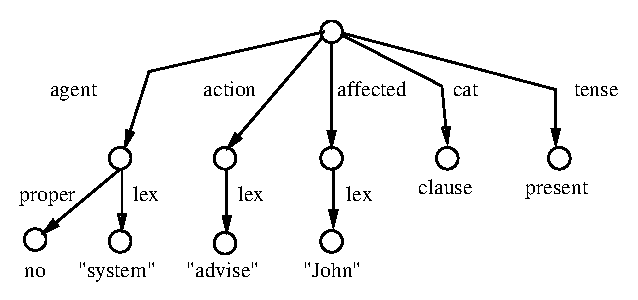
\includegraphics[width=5in, height=2.6in]{graph12.eps}
    \caption{FD as a graph}
    \label{fig3:graph1}
\end{figure}

The graph notation is particularly useful to interpret relative paths. 
When a relative path occurs somewhere in an FD, its destination can be
identified by  going up on the arcs, one arc for each "{\tt \^{}}". 
When the value of a pair is a path, e.g., {\tt (a \{b\})}, then 
the corresponding arc actually points to the same node as the
given path. In this case, there is structure sharing between a and b. This
configuration is illustrated in Fig.\ref{fig3:graph2}, where the paths
{\tt \{action number\}} and {\tt \{agent number\}} are conflated, as well as the
paths {\tt \{affected lex\}} and {\tt \{affected head lex\}} and {\tt \{subject\}} and
{\tt \{agent\}}.  

%\pic{file="graph22.ps", tag=fig3:graph2, cap="Conflation in an FD graph", w=5in, h=2.8in}
\begin{figure}[p]
    \centering
    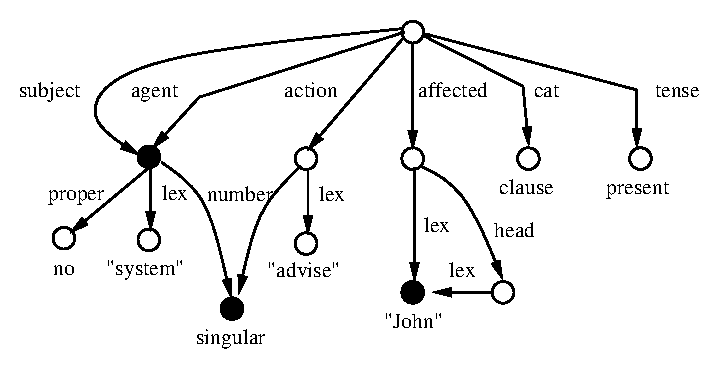
\includegraphics[width=5in, height=2.8in]{graph22.eps}
    \caption{Conflation in an FD graph}
    \label{fig3:graph2}
\end{figure}

The conflation of {\tt \{subject\}} with {\tt \{agent\}} makes all the paths that
are extensions of either {\tt agent} or {\tt subject} equivalent.  For example,
{\tt \{agent lex\}} and {\tt \{subject lex\}} are equivalent.  This equivalence is
easily read in the graph notation.

%\pic{file="graph32.ps", tag=fig3:graph3, cap="A grammar for conjunction", w=5in, h=2.5in}
\begin{figure}[p]
    \centering
    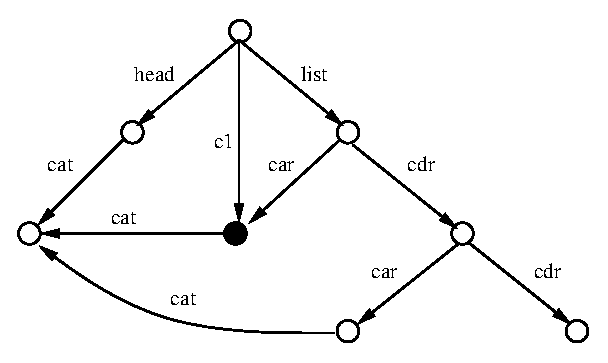
\includegraphics[width=5in, height=2.5in]{graph32.eps}
    \caption{A grammar for conjunction}
    \label{fig3:graph3}
\end{figure}

\label{relpath-ambiguity}
\index{ambiguity of the \^{} notation}
\index{\^{} notation (ambiguity)}
The graph notation also makes it clear that the up-arrow notation can be
ambiguous.  Whenever a Y configuration is met in the graph, for example in
the two black nodes in Fig.\ref{fig3:graph2}, the up-arrow does not specify
which branch of the Y must be taken.  This problem is illustrated in the
grammar in Fig.\ref{fig3:graph3}. The FD is extracted from a grammar
dealing with conjunction.  The constraint enforced by the grammar is that
all the conjuncts in a conjunction must have the same syntactic category.
A conjunction is represented by an FD with two constituents: {\tt head}
represents the conjunction as a whole as a constituent and {\tt list} is a
list of conjuncts.  The list is represented in a singly-linked list of
elements, with a recursive FD containing at each level the first element of
the list (feature {\tt car}) and the rest of the list (feature {\tt cdr}).  In
Fig.\ref{fig3:graph3}, the path {\tt c1} is used to point to the first
constituent of the list.  {\tt c1} is therefore defined by the equation
{\tt {c1} = {list car}}.  The grammar in \textsc{Lisp} notation is shown below
along with a sample input:

\begin{lstlisting}[language=Lisp]

GR =	((c1 {^ list car})
	     (c1 ((cat {^ ^ head cat}))))

IN =	((head ((cat np)))
		 (list ((car ((lex "cat")))
				(cdr ((car ((lex "dog")))
					  (cdr none))))))

\end{lstlisting}

The expression (c1 ((cat ...))) corresponds to the black dot in the graph notation
shown in Fig.\ref{fig3:graph3}.  The problem is to interpret where the
relative path {\tt \{\^{} \^{} head cat\}} is pointing to.  The notation is ambiguous
between {\tt \{head cat\}} and {\tt \{list head cat\}}, depending on whether one
considers the black dot as being located at address {\tt \{c1\}} or {\tt \{list
car\}}.  This ambiguity is solved in FUF by following the convention that
up-arrows always refer to the textual location where they appear in the
grammar.  So in this example, the up-arrows refer to the address {\tt \{c1
cat\}} and not to the address {\tt \{list car cat\}} because they are written as
a pair {\tt (c1 ((cat \{\^{} \^{} head cat\})))} and not as {\tt (list ((car ((cat \{\^{} \^{}
head cat\})))))}.

There are special attributes and values which cannot be drawn in this graph
notation because they have a special unification behavior.  These are, for
attributes: {\tt alt, opt, ralt, pattern, cset, fset, test, control} and
{\tt cat} (or the currently specified cat attribute) and for values:
{\tt none, any} and {\tt given}.  The special constructs {\tt \#(under x)} and
{\tt \#(external y)} have also a special meaning for the unifier.  These are
all the ``keywords'' known by the unifier.  They are presented in the
following sections.


\section{Functional Descriptions vs. First-order Terms}

To conclude the characterization of FDs as a data-structure, it is useful
to contrast functional unification (FU) with the more well known structural
unification (SU) as used in \textsc{Prolog} for example, and to distinguish FDs
from the first-order terms used in SU.

The most important difference is that functional unification is not based
on order and length.  Therefore, {\tt \{a:1, b:2\}} and {\tt \{b:2, a:1\}} are
equivalent in FU but not in SU, and {\tt \{a:1\}} and {\tt \{b:2, a:1\}} are
compatible in FU but not in SU (FDs have no fixed arity).  The following
quote from Knight summarizes the distinction between feature structures and
the first order terms used in SU  \cite[p.105]{Knight}:
\begin{itemize}
\item Substructures are labeled symbolically, not inferred by argument position.

\item Fixed arity is not required.

\item The distinction between function and argument is removed.

\item Variables and coreference are treated separately.
\end{itemize}

A comparison between the FD notation and the first-order term notation
illustrates these differences.  The following FD and first-order term can
be used to represent the fact that {\em Steve builds a crane that is 2 lbs
and 4 feet high}:

\begin{lstlisting}
	((process build)
	 (agent Steve)
	 (object ((concept crane)
                   (weight 2)
                   (height 4))))

	build(Steve, Crane(C1, 2, 4))
\end{lstlisting}

Other representations are of course possible using first-order notation.  Some of them have some of
the advantages of features structures.  For example: 
\begin{lstlisting}
build(B1), 
agent(B1, Steve), 
object(B1, C1), 
crane(C1), 
weight(C1, 2), 
height(C1, 4).
\end{lstlisting}
In fact, any FD can always be translated in a one-to-one mapping to a class of restricted first-order terms.

Contrasting these two notations for the same example illustrates the differences: 
\begin{itemize}

\item {\em Symbolic labels for substructures}: the arguments, that is the {\tt agent}
and the {\tt medium}, are clearly labeled in the feature structure notation.
In particular, a term like {\tt Crane(C1, 2, 4)} is particularly difficult
for a human to interpret.

\item {\em Fixed arity}: features can be added at will to an FD.  FDs are used to
represent {\em partial information}.  This is not the case for first-order
terms.  If the knowledge representation changes to include width to crane
descriptions, in addition to weight and height, all the terms need to be
updated, since {\tt Crane(n, w, h)} is not compatible with {\tt Crane(n, w, h,
l)}.  The FD notation is always partial and leaves the possibility of
adding new features as needed.

\item {\em Function and argument}: first-order terms have a head (the function)
which plays a central role in the unification process.  This is not the
case in FDs.  All information plays the same role.\footnote{In most cases,
however, one feature plays a special role: for example, the {\tt cat}
attribute can specify the category or type of a description, but this is
not built into the syntax, and several such ``special'' attributes can
coexist in the same FD, allowing a reader to adopt several perspectives on
the same FD.}

\item {\em Variables and coreference}: in standard unification, a variable is used
to mean two distinct things: that the value of the role is unknown (there
are no constraints on it), and that the value of the role is the same as
all other objects referred to with the same variable.  So for example, in a
term such as {\tt like(X, X)}, the use of the variable {\tt X} means that we
don't know who likes whom, and that it is known that the agent and the
object of {\tt like} must be the same objects.  The distinction between these
two functions of variables is best explained in \cite{Ait-kaci}.  In FDs,
coreference and unspecification are represented by two different syntactic
devices: variables are features which are unspecified (they simply do not
appear in the FD, or appear with an empty value), coreference is handled
with {\em paths}.  For example, to express the constraint that the medium of
{\tt like} must refer to the same object as its agent, the following FD can
be used:
\begin{lstlisting}
   ((process like)    
    (agent {object})) 
\end{lstlisting} 

\end{itemize}



\section{Disjunctions: The ALT and RALT Keywords}
\index{disjunction} \index{alt (keyword)} \index{ralt (keyword)}


{\tt alt} stands for ``alternation''. The syntax for using {\tt alt} is:

\begin{lstlisting}[language=Lisp]
((att1 val1) 
 (att2 val2)
   ... 
 (ALT {annotations*} (fd1 fd2 ... fdn)) 
   ... 
 (attn valn))
\end{lstlisting}

The meaning of a pair with an {\tt alt} attribute is the following: the
unifier tries to unify the total FD by replacing first the pair {\tt alt} by
the FD {\tt fd1}, if this unification fails, then the unifier will try the
following alternatives.  If all branches of the {\tt alt} fail, the
unification fails.
\index{failure (of unification)}

The order in which branches are put within the {\tt alt} does not change the
result of the unification. (This is an important feature of the process
of unification: the result is always order-independent.) 
\index{order independence} \index{default (in alt)}
However, since only the first successful unification is returned, order
can be used to specify default values. For example, if you want to specify
that a sentence should be at the active voice by default, the following
order should be used:

\begin{lstlisting}[language=Lisp]
(ALT (((voice active)
       ...)
      ((voice passive)
       ...)))
\end{lstlisting}

When the order is truly not relevant and there is no reason to choose a
default branch, then you can use the {\tt ralt} keyword instead of {\tt alt}.
{\tt ralt} has exactly the same syntax as {\tt alt} and also expresses a
disjunction, but the unifier will choose one of the branches at random
instead of always trying the first untried branch.  (ralt stands for
``random alt'')

Alternatively, the :order annotation can be used to specify whether the
branches should be order in random or sequential order.  The syntax is as
follows:
\index{order (annotation)}
\index{order (annotation)}

\begin{lstlisting}[language=Lisp]
(alt (:order :sequential)     is equivalent to  (alt (fd1...fdn))
  (fd1 ... fdn))

(alt (:order :random)         is equivalent to (ralt (fd1...fdn))
  (fd1 ... fdn))

\end{lstlisting}

An {\tt alt} can be embedded within another {\tt alt} or it can be the value of
a feature as in:

\begin{lstlisting}[language=Lisp]
((a (alt (1 2 3 4))))
\end{lstlisting}



\section{Optional Features: the OPT Keyword}
\index{optional features}
\index{opt (keyword)}

{\tt opt} is used to indicate that a set of features is optional. The syntax is

\begin{lstlisting}[language=Lisp]
((att1 val1) 
     ... 
 (OPT fd) 
     ... 
 (attn valn))
\end{lstlisting}

Its meaning is: if the unification of the whole FD succeeds with fd, it is
returned as the result. If it fails, the unifer tries again without fd.
Since the FD nil can be unified successfully with any other FD, {\tt opt} is
a more readable equivalent to the form:

\begin{lstlisting}
(ALT (fd nil))
\end{lstlisting}

{\tt opt} is used exactly in the same way as {\tt alt}.


\section{Control of the Ordering: the PATTERN Keyword}
\label{sect-pattern}
\index{pattern (keyword)}
\index{ordering constraints}

As mentioned previously, the generation of a sentence includes two
subprocesses: unification and linearization.  Unification produces a
complex description of a sentence, made of several constituents.  Each
constituent is described by an FD, and can recursively contain other
subconstituents.

Linearization takes such a complex non-ordered description and outputs a
linear, ordered, string of words. This operation is constrained by
directives put within the FD. These constraints on the ordering appear
after the special attribute {\tt pattern}.
\index{linearization}

For example, in a sentence containing the constituents {\tt prot,
goal} and {\tt verb}, the following {\tt pattern} can be used:

\begin{lstlisting}
(PATTERN (PROT VERB GOAL))
\end{lstlisting}

This means that the linearizer should output a string made of the
linearization of the constituent {\tt prot} first, followed by the
linearization of the constituent {\tt verb} and terminated by the
linearization of the constituent {\tt goal}.  It also means that nothing can
come before {\tt prot} and after {\tt goal}, and nothing can come between each
pair.

The constituents correspond to features of the FD describing the
sentence.  That is, this FD must contain pairs with the
attributes {\tt prot, verb} and {\tt goal}.  For example:

\begin{lstlisting}[language=Lisp]
((cat S)
 (PROT (...))
 (GOAL (...))
 (VERB (...))
 (PATTERN (PROT VERB GOAL)))
\end{lstlisting}

If a constituent mentioned in the pattern is not present in the FD, nothing
happens:  the linearization of an empty (or non existent) constituent is
the empty string.  

The {\tt pattern} directives are generally added by the grammar, since the input
to the unifier should be a semantic representation and therefore does not
contain any constraint on word ordering. 

NOTE: Patterns can contain full paths to specify constituents. For example,
the following is a legal pattern:
\begin{lstlisting}
(PATTERN ({prot n} {verb v} goal))
\end{lstlisting}

A given grammar can generate several constraints, that is it can add 2 or
more {\tt pattern} pairs to the result. The unifier therefore includes a 
{\tt pattern} unifier. The role of the pattern unifier is to take several 
constraints on the ordering and to output one ordering that subsumes all
of them. 
\index{pattern (unification)}

The following symbols have a special meaning for the pattern
unifier: {\tt dots} and {\tt pound} (standing respectively for the
notations `...' and `\#').
\index{dots notation}
\index{pound notation}
\index{dots (in pattern)}
\index{pound (in pattern)}

A pattern {\tt (c1 ... c2)} (noted in the program {\tt (c1 dots c2)})
indicates that the constituent {\tt c1} must precede the
constituent {\tt c2}, but they need not be adjacent. Zero, one or
many other constituents can come in between.  The pattern {\tt (c1
... c2)} still requires the sentence to start with constituent
{\tt c1} and to end with {\tt c2}. The pattern {\tt (... c1 ... c2 ...)}
only forces {\tt c1} to come before {\tt c2}.

The {\tt pound} (\#) symbol is used to represent 0 or 1 constituent.
For example, if you want to allow a sentence to start with an
optional adverbial, you can specify it with the pattern {\tt (\# prot
... verb ...)}. This directive will be compatible with both {\tt (prot
verb goal)} and {\tt (adverb prot verb goal)} for example.

As a consequence of the use of the two symbols {\tt pound} and
{\tt dots}, the constraints described by {\tt pattern} directives are PARTIAL
orderings. 

NOTE: because of the presence of dots and pound, the unification of
patterns is a non-deterministic operation. It can produce several results
for a given input, and there is no way to predict in which order these
possible solutions will be tried. Caution should be exercised when
specifying patterns: they should be specific enough to allow only
acceptable word orderings (do not use too many {\tt dots}) but should not be
too specific to allow for as yet not supported constituents (for example, a
sentence can start with an Adverbial, not necessarily an NP).
\index{non-deterministic constructs}

The following example illustrates the fact that pattern unification is
non-deterministic in general:

\begin{lstlisting}[language=Lisp]
;; Pattern Unification:
p1: (pattern (dots a dots b dots))
p2: (pattern (dots c dots d dots))

;; Compatible Results:
(pattern (dots a dots b dots c dots d dots))
(pattern (dots a dots c dots b dots d dots))
(pattern (dots a dots c dots d dots b dots))
(pattern (dots c dots a dots b dots d dots))
(pattern (dots c dots a dots d dots b dots))
(pattern (dots c dots d dots a dots b dots))

;; Pattern Unification:
p3: (pattern (dots a dots b))
p4: (pattern (dots b c))
;; Pattern Unification fails.
\end{lstlisting}

Patterns are eventually interpreted by the linearization component to
produce a string out of an FD.

Appendix \ref{advanced} describes some advanced uses of pattern unification.


\section{Explicit Specification of Sub-constituents: the CSET Keyword}
\index{cset (keyword)}
\index{constituent traversal}
\label{cset-expansion}

The unifier works top-down recursively: it unifies first the top-level FD
against a grammar (generally the top-level FD represents a sentence), and
then, recursively, it unifies each of its constituents. For example, to
unify a sentence, the unifier first takes the whole FD and unifies it with
the grammar of the sentences {\tt (cat S)}, then it unifies the {\tt prot} and
{\tt goal} with the grammar of NPs {\tt (cat np)}, then it unifies the {\tt verb}
with the grammar of VPs {\tt (cat vp)}.
\index{recursion} \index{constituent}

You can specify explicitly which features of an FD correspond to constituents
and therefore need to be recursively unified. To do that, add a pair:

\begin{lstlisting}[language=Lisp]
(CSET (c1 ... cn))

;; For example:
(CSET (PROT VERB GOAL))
\end{lstlisting}

The value of a {\tt cset} (stands for Constituent SET) is considered as a SET
(unordered). Therefore the following 2 pairs are correctly unified:

\begin{lstlisting}[language=Lisp]
(CSET (PROT VERB GOAL))
(CSET (VERB GOAL PROT))
\end{lstlisting}

Actually, two {\tt cset} pairs are unified if and only if there
values are two equal sets.
\index{cset (unification)}

NOTE: A {\tt cset} values can contain full paths to specify constituents. So
for example, the following is a legal feature:

\begin{lstlisting}[language=Lisp]
(cset ({prot n} {verb v} goal))
\end{lstlisting}

FUF does not rely exclusively on {\tt cset}s to find the constituents to be
recursively unified. FUF generally tries to infer the value of {\tt cset} from
the value of {\tt pattern} and an observation of the features of the current
FD (with the assumption that features containing a {\tt cat} attribute are
constituents).  The exact procedure followed to identify the implicit
constituent set of an fd is:
\begin{enumerate}
\item If a feature {\tt (cset (c1 ... cn))} is found in the FD, the constituent set
is just {\tt (c1 ... cn)}.

\item If no feature {\tt cset} is found, the constituent set is the union of the
following sub-fds:
\begin{enumerate}
\item If a pair contains a feature {\tt (cat xx)}, it is considered a constituent.

\item If a sub-fd is mentioned in the pattern, it is considered a constituent.
\end{enumerate}
\end{enumerate}

As a consequence, explicit {\tt cset}s are rarely necessary.  They are
generally used when an fd contains a sub-fd that either is mentioned in the
pattern or contains a feature {\tt cat}, but that you do NOT want to unify.
In that case, you can explicitly specify the cset without including this
unwanted sub-fd.  For larger grammars, however, you should put the emphasis
on a clean constituent structure, and therefore you should carefully use
the explicit CSET facilities instead of blindly relying on FUF's
inferencing.  In this case, the advanced CSET facilities described below
will prove helpful.

\subsection{Implicit and Incremental CSET Specification}
\label{incr-cset}

CSET specification is the means by which a programmer describes the
constituent structure of sentences.  Given the importance of this task and
its complexity, facilities have been added to FUF to make CSET
specification more flexible.  It is thus possible to specify {\em implicit}
and {\em incremental} CSETs.  This section describes these features of the
CSET specification.  It presents advanced facilities and can be skipped in
first lecture.

The general form of a CSET specification is:
\begin{lstlisting}[language=Lisp]
(CSET (= c1 ... cn)
      (== b1 ... bm)
      (+ a1 ... ap)
      (- d1 ... dq)))
\end{lstlisting}

The simple syntax {\tt (CSET (c1 ... cn))} is equivalent to 
{\tt (CSET (= c1 ... cn))}. 

As usual in FDs, all of the features of the CSET are optional.
Each feature in the CSET feature is named as follows:
\begin{itemize}
\item The = sublist is called the absolute CSET.  

\item The == sublist is called the basis CSET.

\item The + and - sublists are the increment CSETs.
\end{itemize}

The idea behind the use of incremental CSETs is to gradually refine the
CSET description, by adding partial information - thus folding the
constituent structure description into the general ``partial information,
gradual refinement'' methodology of FD specification.  The incremental CSET
specifications are added to the basis CSET, which can either be specified 
explicitly, using the == notation, or be the result of the implicit CSET
inference described above.

The actual CSET of an FD is computed by applying the following procedure:
\begin{enumerate}
\item If the absolute CSET (=) is present, it becomes the value of the actual
CSET.  The absolute CSET feature is used when you want to disable all
incremental computations.

\item Else: If the basis-CSET is present, 
\begin{enumerate}
\item let BSET = basis-CSET, else let BSET = the implicit CSET, computed as
described above (from pattern and cat inspection).

\item If the +increment-CSET is present, let BSET = BSET union +increment.

\item If the -increment-CSET is present, let BSET = BSET - -increment (set
difference). 

\item Return BSET as the actual CSET.
\end{enumerate}
\end{enumerate}

The result of this procedure is a list of absolute paths, pointing to the
sub-constituents of the current constituent.  In all cases, this actual
cset is ``cleaned up'' by applying the following procedure:
\begin{itemize}
\item All duplicate paths are removed.  Two paths are duplicate if
they point to the same FD.  That is, even if the paths are distincts but
they point to conflated FDs, they are considered duplicates in the CSET.

\item All leaf-constituents are removed.  A leaf-constituent is a constituent
whose value is not a list of pairs - for example, a symbol or a string.
The idea is that there is no point in recursing on a leaf-constituent.

\item All constituents which are conflated with a -increment constituent are
also removed from the actual cset.
\end{itemize}

The following grammar fragments illustrate briefly the use of incremental
CSET specification.\footnote{Keep in mind that this facility is above all designed
for use in large grammars, and the short fragments shown here could easily
be handled without incremental CSETs.}

\begin{lstlisting}[language=Lisp]
((cat clause)
 (cset (== prot verb))
 (alt (((prot given)
        (subject {^ prot})
        (voice active))
       ((prot none)
        (goal given)
        (cset (- prot) (+ goal))
	(subject {^ goal})))))
\end{lstlisting}

The first cset feature specifies that the basis cset for this clause
constituent should {\em not} be the implicit cset (derived from pattern and
cat), but instead the explicit list (prot verb).  In the second cset
feature, this basis cset is incrementally refined by specifying that when
prot in none, prot is not part of the cset and instead goal is added to the
cset.  If prot is a non-leaf constituent, then the actual cset for this
example will be (prot verb), if it is none, then it will be (verb goal).

\begin{lstlisting}[language=Lisp]
((cat clause)
 (subject ((cat np)))
 (prot {^ subject})
 (cset (- prot)))
\end{lstlisting}

In this second fragment, no absolute cset is specified (no = feature) and
no basis cset is present (no == feature).  Therefore the implicit cset is
computed and is found to be (subject) (because of the presence of the (cat
np) feature under subject).  (subject) is thus the initial basis-cset.  The
incremental cset (- prot) is then added to the cset.  The basis-cset
remains (subject) at this point.  Finally, the cset is ``cleaned'' - and it
is found that prot and subject are duplicates of each other because of the
conflation (prot \{\^{} subject\}).  Since prot is member of the -increment
list, its ``synonyms'' are deleted from the basis cset, and the actual cset
is found to be empty ().

The computation of implicit and incremental CSETs can interact with the
more advanced control features of goal freezing (with the {\tt wait}
construct).  These interactions are described in Sect.\ref{wait-cset}.


\subsection{Unification of Incremental CSET Specifications}
\index{cset (unification)}

When two complete CSET specifications are unified, the following rules are
applied:  assume that (cset (= a1) (== b1) (+ c1) (- d1)) is unified with 
(cset (= a2) (== b2) (+ c2) (- d2)),
\begin{enumerate}
\item If both a1 and a2 are instantiated:
\begin{enumerate}
\item If (set-equal a1 a2) then:
\begin{enumerate}
\item If c1 union c2 is included in a1, return (cset (= a1))
Else return :fail.

\item If d1 union d2 intersect with a1, return :fail
Else return (cset (= a1))
\end{enumerate}

\item else :fail.
\end{enumerate}

\item If only a1 is instantiated and a2 is null:
\begin{enumerate}
\item If a1 intersects d1 union d2, then :fail.

\item Else (cset (= a1)) is returned.
\end{enumerate}

\item If neither a1 and a2 is instantiated, compute the unions: b=b1 u b2, c=c1 u
c2, d = d1 u d2, and return (cset (== b) (+ c) (- d)).
\end{enumerate}




\section{The Special Value NONE}
\index{none (special value)}

There is a way to prevent an FD from ever getting a value for a
given attribute. The syntax is: {\tt (att NONE)}.  It means that
the FD containing that pair will NEVER have a value for \t'att'.
Or in other words, that the object described by the FD has no
attribute \t'att'.


\section{The Special Value ANY - The Determination Stage}
\label{determination}
\index{any (special value)}
\index{determination}
\index{total fd}
\index{instantiated features}

An {\tt any} value in a pair means that the feature must have a
determined value at the end of the unification. A complete
unified FD will never contain an {\tt any}, since an {\tt any} stands
for something that must be specified. If after unifying
everything, the resulting FD contains an {\tt any}, then the
unification fails.
\index{failure (of unification)}

An {\tt any} represents a strong constraint. It means that a feature MUST be
instantiated. {\tt any} should not be understood as ``the feature has a value
in the input'' but as ``the feature WILL have a value in the result.''

The idea of a ``resulting final FD'' coming out of the unification is 
important. It actually implies that the process of unification is the
composition of 2 sub-processes: the unification per se and what we call
here the ``determination.''

The determination process assures that the resulting FD is well formed.  It
is a necessary stage since the ``resulting final'' FD is more constrained
than regular FDs. Here is what the determination does:
\begin{itemize}
\item checks that no {\tt any} is left.

\item tests all the {\tt test} constraints. \index{test (keyword)}

\item tests that no frozen constraint is left. \index{wait (control annotation)}
\end{itemize}

\index{determination}
It is important to realize that none of this can be done before the 
unification is finished.  Section \ref{wait-cset} gives a more complete
picture of the determination process and explains why there may be a need
for several cycles of determination when {\tt wait} and goal freezing are
used. 

Note that in practice, ANY is used rarely.  The next special value GIVEN is
used more often, and is easier to manipulate, except in cases where goal
freezing is used.


\section{The Special Value GIVEN}
\index{given (special value)}

A {\tt given} value in a pair means that the feature must have a real value
at the beginning of the unification.  A unified fd will never contain a
{\tt given} since {\tt given} will always be unified with a real value.
{\tt given} is useful to specify what features are necessary in an input.  It
is also much more efficient than {\tt any}.  It is often used in branches of
an {\tt alt}, to ``test'' for the presence of a feature.

The rule is: when you think of using {\tt any}, you often want to use
{\tt given} and, conversely, when you use {\tt wait} (for goal freezing) and
something does not work, it is because you should use {\tt any} instead of
{\tt given}.

\index{constituent traversal}
{\tt Given} addresses the most obvious limitation of the top-down regime used
by FUF when traversing the constituent tree (and computing the cset
expansion) in cases when the grammar contains the equivalent of
left-recursive rules.  {\tt Given} is in a sense the dual of the {\tt any}
meta-variable of the original \textsc{FUG} formalism: while {\tt any} requires a
feature to be instantiated at the {\em end} of the unification process,
{\tt given} requires it to be instantiated {\em before} unification starts.
Thus, {\tt given} is used to check that a constraint has been specified in
the input.  A {\tt given} feature can only appear in a grammar, thus,
{\tt given} gives a different status to the two arguments of the unification
function.\footnote{This means that when {\tt given} is used, unification is no
longer symmetric, but it remains order-independent and monotonic.}

\begin{lstlisting}[language=Lisp]
	((cat NP)
	 (semr ((possessor GIVEN)))
	 (cset (det head))
	 (det ((cat NP)
	       (possessive yes)
	       (semr {^ ^ possessor})))
	 ...)
\end{lstlisting}

To illustrate how {\tt given} solves the problem of the left-recursive rules,
consider how the possessive NP rule is implemented in FUF in this example.
This FD implements the FUF equivalent of a rule:
\begin{lstlisting}[language=Lisp]
NP -> NP(possessive) head
\end{lstlisting}

This is a left-recursive rule which, if used in a top-down control, could
lead to infinite recursion of the form $NP \rightarrow NP (NP (NP ..... (NP head...)))$.
Note how the cset expansion in FUF is the equivalent of the rule application in rule-based grammatical formalisms.

To avoid using this rule when there is no possessor in the input (which is
the step which leads to non-termination), the grammar contains a feature
{\tt (possessor GIVEN)}, checking that the semantic representation of this
constituent does indeed have a possessor specified in the input.  If none
is specified, then the rule will fail, and the sub-constituent possessive
NP will not get created.  Without the use of GIVEN, this FD would always be
successfully unified, and the cset expansion would lead to non-termination.
The use of the {\tt given} meta-variable therefore ensures that the top-down
regime of FUF is goal-directed.

NOTE: The {\tt under} construct is related to the {\tt given} value.  It is
presented in Section \ref{feature-type}.  
\index{under (special value)}




\section{The Special Attribute CAT: General Outline of a Grammar}
\index{cat (special attribute)}
\index{grammar organization}
\index{category}

Each constituent of an FD is generally characterized by its ``category''.
In FD terms, this means each constituent includes a feature of the
form {\tt (CAT category-name)}, where category-name is expected to be an atom.

A grammar is expected to give directives for each possible category, for
example NP, VP, or NOUN. The outline of a grammar must be:

\begin{lstlisting}[language=Lisp]
((alt (
       ((cat s)
        <rest of grammar for category S>)
       ((cat np)
        <rest of grammar for category NP>)
       <other categories>
      )))
\end{lstlisting}

NOTE: The current version of the unifier makes the assumption that the
grammar has such a form. The {\tt (CAT xxx)} pairs must appear first.  The
function {\tt grammar-p} checks that a grammar has the right form.  The list
of categories known by the grammar can be found by using the function
{\tt list-cats}. See appendix \ref{sect-non-standard} for a list of the
non-standard features of this implementation.
\index{non-standard features of implementation}
\index{restrictions}

NOTE: The symbol identifying categories ({\tt 'cat}) can be changed in the
program.  It is by default {\tt 'cat}, but this default can be changed by
setting a new value to the {\tt *cat-attribute*} variable or by providing an
optional argument to the unification functions, as explained in the
reference manual.  
\index{\*cat-attribute\* (variable)}
\label{cat-attribute}


\chapter{Modular Organization of Grammars: Def-alt and Def-conj}
\label{def-alt}
\index{def-alt (construct)}
\index{def-conj (construct)}

A large \textsc{FUG}, like many other large computer programs, becomes difficult
to read and maintain when its size increases.  The size of a \textsc{FUG} is
best measured by counting the number of disjunctions it contains, as
discussed in Chapter \ref{complexity}.  \index{complexity}
The depth of embedding of the disjunctions is also an indication of the
complexity.  The number of branches in the disjunctive normal form of the
grammar accounts for this embedding but is in general not very informative.
For example, the grammar of FUF contains 580 disjunctions and has a
disjunctive normal size of $10^{29}$.  Another more conventional measure of
the complexity of the grammar viewed as a program, is the number of lines
of code: 9,500 lines for a total of 290,000 characters.  By all measures,
such a grammar is a large program.  So the well-known problems of size
management in software engineering become an issue for large \textsc{FUG}s: ease
of maintenance, readability, modularity etc.

\section{Modular Definition of FDs}

A \textsc{FUG} is a large FD containing many alternations.  At the top-level, a
\textsc{FUG} is conventionally made up of a large alternation where each branch
describes a different category.  The pattern is:
\begin{lstlisting}
	((alt (((cat clause) ...)
	       ((cat noun-group) ...)
	       ((cat verb-group) ...)
	       ...)))
\end{lstlisting}

Each branch is an embedded FD containing in turn many disjunctions.  For
example, the top-level clause grammar is made up of the following
alternations:
\begin{lstlisting}
	((cat clause)
	 (alt mood ...)
	 (alt transitivity ...)
	 (alt voice ...)
	 (alt circumstantial ...)
	 (alt displaced-constituent ...)
	 ...)
\end{lstlisting}
Each one of these alternation in turn is a large FD, with many embedded
alternations.  

FUF includes a very simple mechanism to allow the grammar writer to develop
such large grammars in a modular way.  The key aspect is to allow the
grammar writer to abstract away from the details of an FD by giving it a
name.  Named FDs can then be used anywhere a regular FD is allowed.
Actually, it turned out that instead of using named FDs, named features
were much more convenient.  The new syntax distinguishes between two types
of named features: named disjunctions and named conjunctions defined by
{\tt def-alt} and {\tt def-conj} respectively.  Named features can then be used
in any FD as regular features; that is, instead of a pair, an FD can
contain a named feature.  The syntax is illustrated below:

\begin{lstlisting}[language=Lisp]
(def-alt number (:index number)
   (((number singular) ...)
    ((number plural) ...)))

(def-conj agreement-3-sing-masc
   (number singular)
   (person third)
   (gender masculine))


;; Using named feature         Expanded form

((alt (((cat noun-group)       ((alt (((cat noun-group)
        (:! number)                    (alt (:index number)
        ...))))                          (((number singular) ...)
                                          ((number plural) ...)))
                                           ...))))

((head ((lex "man")))          ((head ((lex "man")))
 (:& agreement-3-sing-masc))    (number singular)
                                (person third)
                                (gender masculine))
\end{lstlisting}

\index{def-alt (construct)}
\index{def-conj (construct)}
\index{! (notation)}
\index{\& (notation)}

A reference to a named disjunction has the form {\tt (:! name)}; {\tt (:\&
name)} is used for named conjunction.  These forms can appear anywhere a
pair could appear in an FD.  A named conjunction works like a bundle of
features which get spliced in the embedding FD when it is referenced.  A
named disjunction accepts all the annotations that an alt can carry
(control and tracing annotations).  The {\tt def-alt} and {\tt def-conj}
mechanism works as a macro mechanism for grammars.

This simple syntactic tool allows the use of abstraction in the development
of \textsc{FUG}s: by naming parts and hiding levels of details, the structure of
the grammar becomes more apparent.  Named features can be re-used in
different contexts (several places in the grammar and/or in several
grammars).  Practically, it becomes possible to work separately on a module
of the grammar without affecting the other parts; several people can work
together on the same grammar; single modules can be re-loaded and
re-defined without requiring re-loading the whole grammar.  The standard
benefits of modularity in programming languages apply to the full extent.

\section{Drawing the Map of a Grammar}

Interestingly, the new syntax highlights the similarity between \textsc{FUG}s
and the systems of systemic linguistic.  FUF includes a tool that draws a
graphical map of the grammar by displaying the tree of the named features
with their dependents (function {\tt draw-grammar}).  A high-level map of the
SURGE grammar is shown below.  Note how similar this map is to a system in
systemic linguistics.  The {\tt def-alt} syntax has made this level of
organization clearly visible in the grammar without requiring any change to
the FUF formalism.

The functions which produce this type of grammar maps in either character
mode or in postscript format are described below:

\begin{lstlisting}[language=Lisp]
DRAW-GRAMMAR (&optional (root *u-grammar*))
;;	Draw the map of a grammar, starting at level root (by default the 
;; 	root of the whole grammar).

FUF-POSTSCRIPT (root filename &key (shrink t))
;;	Produces a postscript file depicting the map of a grammar.
;; 	If shrink is t, the map is forced to fit on a single page.

;; Example of output:

> (draw-grammar 'det)
|- DET +
       |- PRE-DET
       |- DEICTIC2
       |- ORDINAL
       |- QUANTIFIER
       |    +
       |    |- QUANT-COUNT-PLURAL
       |    |    +
       |    |    |- QUANT-PARTITIVE
       |    |    |- QUANT-PARTITIVE
       |    |    
       |    |- QUANT-MASS
       |    |    +
       |         |- QUANT-PARTITIVE
       |         
       |    
       |- DET-TYPE +
                   |- ARTICLE-DET
                   |- POSSESSIVE-DET
                   |- QUESTION-DET
                   |- DEMONSTRATIVE-DET
                   |- QUANTIFIER-DET
                   
       
\end{lstlisting}
\index{draw-grammar (function)}
\index{fuf-postscript (function)}


\begin{figure}[t]
	\centering
	% \includegraphics{boundingbox="0, 0, 612, 790", scaletofit, width = 6.5 in, height = 8.5in, Postscript=grammar-map.ps}}
	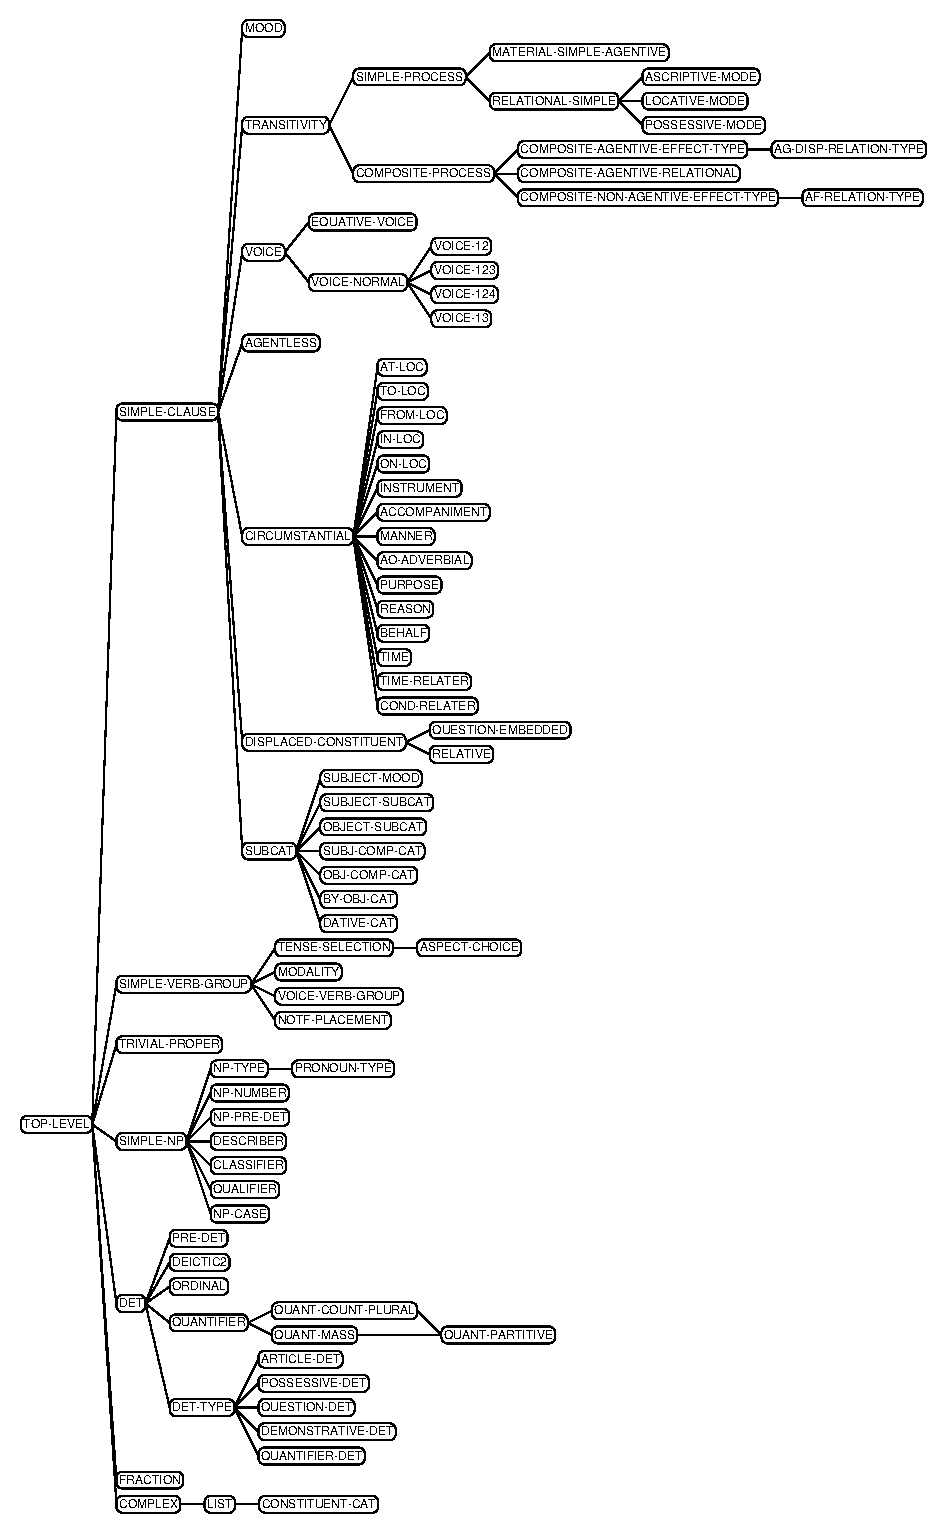
\includegraphics[width=6.5 in, height=8.5in]{grammar-map.eps}
	\caption{Map of the SURGE grammar using the def-alt syntax}
\end{figure}


\chapter{Defining Input for Regression Testing: The Test Facility}

When developing a grammar, it is important to check that existing input
configurations remain compatible whenever the grammar is changed.  To this
end, FUF includes a regression testing mechanism an a test system.  This
system allows the grammar developer to define a set of test cases, which
are pairs of input FDs together with the sentence they are expected to
produce.  The test system allows to run a series of tests and checks
whether the output is equal to the expected output, it can in addition
measure the time spent on each test.  A final advantage of the test
facility is that test definitions can use the :\& notation and therefore big
FD specifications can be written modularly.


The following functions are defined to take advantage of this facility:

\begin{lstlisting}[language=Lisp]
(def-test name result input) 
;; Define a named test: test on input should produce result. 
;; If result is a list, testing result can produce any one of the elements
;; of result.

(get-test name)
;; Return the input for named test.

(clear-tests)
;; Remove all test definitions.

(test &key from to item timed)
;; Evaluate a sequence of tests.
;; A test calls uni-string on input and compares the result with the test's
;; result. 
;; If timed is non-nil, time all tests.
;; from and to identify first and last tests in order in which they have
;; been defined.
;; item: identify tests explicitly - either one name or a list of names.

;; Examples:
(def-test :from 't1 :to 't212)
(def-test :item '(t6 t9 t45) :timed t)
(def-test :item 't6)
\end{lstlisting}

When running the tests, the following output is produced:

\begin{lstlisting}[language=Lisp]
FUG5 12> (test :item '(t1 t14 t212))

====================
T1 --> "This car is expensive."

{Used 117 backtracking points - 26 wrong branches - 15 undos}

{Used 119 backtracking points - 26 wrong branches - 15 undos}
OK
====================

T14 --> "For her to do it."

{Used 152 backtracking points - 36 wrong branches - 13 undos}

{Used 158 backtracking points - 36 wrong branches - 13 undos}
OK
====================

T212 --> "What."

{Used 39 backtracking points - 12 wrong branches - 4 undos}

{Used 40 backtracking points - 12 wrong branches - 4 undos}
OK
====================

3 tests run - 3 correct.
\end{lstlisting}

If a test does not succeed, the following output is produced:

\begin{lstlisting}[language=Lisp]
FUG5 14> (test :item 't1bis)

====================
T1BIS --> "This car is not expensive."

{Used 117 backtracking points - 26 wrong branches - 15 undos}

{Used 119 backtracking points - 26 wrong branches - 15 undos}
Expected "This car is not expensive."
Instead  "This car is expensive."
====================

1 test run - 0 correct.
The following tests are incorrect: (T1BIS)
\end{lstlisting}



\chapter{Using Lists in FDs}
\label{fdlist}

Lists of objects are not a primitive type in FUF.  The reason is that a
list of FDs is not a legal FD.  Lists are however very useful in
grammatical description, when dealing with subcategorization or
conjunction.  FUF therefore contains some built-in support for the
expression and manipulation of lists.  The issue of list manipulation is
further developed in Appendix \ref{prolog}, where list processing is used
as an example showing the expressive power of FUF as a programming
language.  

This chapter explains how and when to use lists in FUF and describes the
FUF facilities easing the use of lists.

\section{Encoding Lists as FDs}

A list of FD l = (fd1, fd2 ... fdn) is not a legal FD according to the
definition of FDs.  The main reason why such a form is not accepted in the
syntax of FUF is that defining what should be the unification of two lists
(fd11, fd12 ... fd1n) and (fd21, fd22, ... fd2p) is not clear (should it be
the union of the 2 lists, its intersection using unification as an equality
test, the pairwise unification of the elements one by one, or the product
of the unifications, what happens when one unification of the elements
fails...) and it is not clear how to extend the notion of path to allow
access within a list.

Instead of adding lists as a primitive type of FDs, it is possible to
encode lists as regular FDs.  This is the approach used and supported in
FUF.\footnote{Note that it is also possible to define lists as procedural
types, with any desired specialized unification procedure.  But in that
case, lists are used as black boxes into which path expressions cannot
enter.} 

Quite simply, lists are represented as FDs with two features,
CAR and CDR (with names ala Lisp). 
\index{car (in FDs)}
\index{cdr (in FDs)}

\begin{lstlisting}[language=Lisp]
;; The list (a b c) is represented by the FD:

((car a)
 (cdr ((car b)
       (cdr ((car c)
             (cdr none))))))

;; The list (a (b c)) is represented by the FD:

((car a)
 (cdr ((car ((car b)
             (cdr ((car c)
                   (cdr none)))))
       (cdr none))))
\end{lstlisting}

When using this encoding for lists, the path notation can be used to access
any element of the list (using a sequence of car and cdr), and the
unification method to use when dealing with lists can be defined
declaratively in the grammar.  FUF includes tools to make the reference to
list elements and the development of list-related grammars easier.

\section{When to Use Lists: an Example}

Lists should be used whenever you are thinking of using feature names of
the form att1, att2 - {\em i.e.}, whenever you want to go around the
limitation of FDs that only one attribute with a given name exist by adding
subscripts to the attribute names.  Natural candidates for the use of lists
are conjunction and the semantic encoding of non-singular objects.  

In the following example, lists are used to encode the logical form of a
sentence.  This encoding encodes in FUF a KL-ONE type of knowledge
representation based on entities and binary relations between these
entities.  

\begin{lstlisting}[language=Lisp]
;; An FD used in Jacques Robin's Basketball Report Writing System
;; This is a list of entities and a list of relations in which they
;; participate. 

;; Semantic content of the sentence:
;; Malone scored 28 points and John Stockton added 27 points and 24 assists.

statistics(malone, 28points)
statistics(stockton, 27points)
statistics(stockton, 24assists)

;; FD notation:

 (setf input
       '((cat semantic)

        ;; note the use of the ~ notation to encode a list of FDs.
		(ents ~(((concept player) (name malone))
				((concept stat) (value 28pts))
				((concept player) (name stockton))
				((concept stat) (value 27pts))
				((concept stat) (value 24asts))))

		;; Note the usage of ^n~ to escape to the beginning of the
		;; containing list and ~n to go down nth elt of a list.
        ;; ^2~ means "go up 2 levels and then to the beginning of the list"
		(rels ~(((concept stat-rel)
				 (args ((carrier {^2~ ents ~1}) 
						(stat {^2~ ents ~2}))))
				((concept stat-rel)
				 (args ((carrier {^2~ ents ~3}) 
						(stat {^2~ ents ~4}))))
				((concept stat-rel)
				 (args ((carrier {^2~ ents ~3}) 
						(stat {^2~ ents ~4})))))))))

\end{lstlisting}


The notation \~{} and \^{}n\~{} are detailed below.  They are used to ease the
writing of lists as FDs and to traverse lists with path expressions.  
In this example, note how the lists ents (for entities) and rels (for
relations) are encoded as regular FDs, and how parts of the ents list are
used in the rels FD (for example, the first element of the rels list
contains two paths to the first and second element of the ents list).  This
form of structure sharing between parts of lists would not be possible
using a ``black box primitive'' list encoding.


\section{Typical List Traversal in FUF}

Once lists are encoded as FDs, grammars need to be defined to traverse the
lists and unify them according to the specific semantic of each list.
Lists are traversed by recursive grammars, using the constituent traversal
mechanism implemented by cset.  The following example shows how to use the
input shown above to build a clause out of the semantic input, by composing
elements of the appropriate type.  The grammar contains the categories
{\tt semantic}, {\tt find1} and {\tt find2}.  The easiest way to explain how this
function works is by taking a procedural interpretation of the FUF flow of
control.  This procedural interpretation is explained in detail in Appendix
\ref{prolog}.  A constituent can be viewed as a procedure, that receives a
certain set of parameters and computes new return values.  In this example,
the constituent {\tt semantic} receives as input the features {\tt ents} and
{\tt rels} which as shown in the FD {\tt input} above.  It computes a new
feature {\tt clause} as output, which is a linguistic constituent.  To this
end, it also uses two local variables stored in the features {\tt ent1} and
{\tt rel1}.  All in all, the function of this category is to map a
description of a semantic content into a linguistic clause description.  

The grammar also implements two other categories, {\tt find1} and {\tt find2},
which are the ones related to list processing.  These categories can be
interpreted as procedures searching a list for one or two matches.  The
simpler one is {\tt find1}.  {\tt Find1} receives two input parameters {\tt in1}
and {\tt 1st-match} which are a list of FDs and an FD.  The category searches
the list for the first-match in the list which can be unified with the
feature {\tt 1st-match}.  When it is found, the feature {\tt 1st-match} and the
element in the list are unified (conflated).  The category {\tt find2}
operates the same way but for two features {\tt 1st-matchA} and
{\tt 1st-matchB}.  


\begin{lstlisting}[language=Lisp]
;; A grammar to find matching elements in the list of semantic binary
;; relations and compose the matched elements into a linguistic clause
;; structure. 
(def-grammar rules ()
 (clear-bk-class)
 '((ALT
    (((cat semantic)
      (ent1 ((cat find2)
	     (in2 {^2 ents})
	     (1st-matchA ((concept player) (name stockton)))
	     (1st-matchB ((concept stat)))))
      (rel1 ((cat find1)
	     (in1 {^2 rels})
	     (1st-match ((concept stat-rel)
			 (args ((carrier {^4 ent1 1st-matchA})
				(stat {^4 ent1 1st-matchB})))))))
      (cset ((= ent1 rel1)))
      (clause ((cat clause)
	       (process stat)
	       (args {^2 rel1 1st-match args}))))

     ;; LIST PROCESSING CONSTITUENTS:
     ;; Find one element in a list in1 that matches 1st-match and unifies
     ;; it with 1st-match.
     ;; If no element in list in1, fail
     ;; If first element matches 1st-match, unify and stop recursion
     ;; Else recurse on rest of in1.
     ;; 1st-match is always linked to the top-level 1st-match feature in
     ;; the embedded structure of recursive calls.
     ((cat find1)
      (fset (in1 1st-match rest cat cset))
      (ALT find1 (((1st-match {^ in1 car})
		   (cset ()))
		  ((rest ((cat find1)
			  (1st-match {^2 1st-match})
			  (in1 {^2 in1 cdr})))
		   (cset ((= rest)))))))

     ;; Find 2 elements in a list in2 that match 1st-matchA and 1st-matchB
     ;; and unify them.
     ((cat find2)
      (fset (in2 1st-matchA 1st-matchB restA restB cat cset))
      (cset ((= restA restB)))
      (restA ((cat find1) 
	      (1st-match {^2 1st-matchA})
	      (in1 {^2 in2})))
      (restB ((cat find1) 
	      (1st-match {^2 1st-matchB})
	      (in1 {^2 in2}))))))))

;; To test:
(setq output (uni-fd (input) (rules)))
(top-gdp output {clause args carrier})
(top-gdp output {clause args stat})
\end{lstlisting}

The list traversal is implemented in the category {\tt find1}.  The grammar
for {\tt find1} contains a typical list recursion, similar to the following
Lisp function:

\begin{lstlisting}[language=Lisp]
(defun find1 (in1 match1)
  (if (equal match1 (car in1))
      match1
      (find1 (cdr in1) match1)))
\end{lstlisting}

Naturally, since the grammar is written in FUF it performs differently, but
the structure is similar.  The {\tt if} test is implemented as an {\tt alt},
and the recursive call is implemented by a cset expansion to the
sub-constituent rest.  This structure is typical of the FUF list traversal
categories and can be found in a similar form in the SURGE segment dealing
with conjunctions.  


\section{Path Notations for Lists}

To make the use of lists more convenient, three special notations have been
defined in FUF: \~{}, \^{}\~{} and \~{}n.  The macro-character \~{} is used to define
lists of FDs as an FD with features car and cdr.  It performs the following
transformation:

\begin{lstlisting}[language=Lisp]
~(fd1 fd2 ... fdn)  <==> ((car fd1)
                          (cdr ((car fd2)
                                (cdr ...
                                          ((car fdn)
                                           (cdr none))))))
\end{lstlisting}


The two other notations are used within path expressions (within curly
braces).  \~{}n is used to access the nth element within a list.  It is
expanded to the appropriate sequence of cdrs and car.  The notation \^{}\~{} is
used to go back up to the beginning of a list from within an element of a
list.  This is expanded at unification-time since it depends on the level
of embedding of the element.  Therefore \^{}\~{} actually increases the
expressive power of path expressions.  If \^{}\~{} is used within a feature which
is not a list element (which means that it does not occur under {\tt car}),
then it is equivalent to the simple \^{} (which means that it does go up one
level anyway).   The shorthand notation \^{}n\~{} is used for \^{}n \^{}\~{} that is, go
up first n levels and then to the beginning of the embedding list.  These
notations are shown for example in the input example above.


\chapter{Types in Unification}

FUF implements three notions of types:
\begin{itemize}
\item Typed features

\item Procedural types with user-defined unification methods

\item Constituent types with the \textsc{FSET} special feature 
\index{fset (special attribute)}
\end{itemize}

The idea of using types in unification is relatively recent.  So we first
motivate the use of types in FUGs.  The following sections describe each
one of the three methods of typing available.

\section{Why Types?}

\subsection{Typed features}

\paragraph{A Limitation of FUGs: No Structure over the Set of Values}

To formally define a grammar, we define $L$ as a set of labels
or attribute names and $C$ as a set of constants, or simple atomic
values. A string of labels (that is an element of $L^*$) is
a path, and is noted $\{l_1 \ldots l_n\}$.  A grammar defines a domain
of admissible paths, $D \subset L^*$. $D$ defines the skeleton of well-formed FDs.

In functional unification, the set of constants $C$ has no structure.  It
is a flat collection of symbols with no relations between each other.  All
constraints among symbols must be expressed in the grammar.  In
linguistics, however, grammars assume a rich structure between properties:
some groups of features are mutually exclusive; some features are only
defined in the context of other features.

\begin{lstlisting}[language=Lisp]
                 | Question
                 | Personal
     | Pronoun --|
     |           | Demonstrative
     |           | Quantified
Noun |
     | Proper
     |           | Count
     | Common ---|
                 | Mass
\end{lstlisting}

Let's consider a fragment of grammar describing noun-phrases (NPs) using
the systemic notation given in \cite{Winograd83}.  Systemic networks, such
as this one, encode the choices that need to be made to produce a complex
linguistic entity.  They indicate how features can be combined or whether
features are inconsistent with other combinations.  The configuration
illustrated by this fragment is typical, and occurs very often in grammars.
The schema indicates that a noun can be either a pronoun, a proper noun or
a common noun.  Note that these three features are mutually exclusive. Note
also that the choice between the features {\tt {question, personal,
demonstrative, quantified}} is relevant only when the feature pronoun is
selected.  This system therefore forbids combinations of the type
{\tt {pronoun, proper}} and {\tt {common, personal}}.

The traditional technique for expressing these constraints in a FUG is to
define a label for each non terminal symbol in the system.  The resulting
grammar is as follows:

\begin{lstlisting}[language=Lisp]
((cat noun)
 (alt (((noun pronoun)
	(pronoun 
	 ((alt (question personal demonstrative quantified)))))
       ((noun proper))
       ((noun common)
	(common ((alt (count mass))))))))
\end{lstlisting}

This grammar is, however, incorrect, as it allows combinations of the type
{\tt ((noun proper) (pronoun question))} or even worse {\tt ((noun proper)
(pronoun zouzou))}.  Because unification is similar to union of features
sets, a feature {\tt (pronoun question)} in the input would simply get added
to the output.  In order to enforce the correct constraints, it is
therefore necessary to use the meta-FD \textsc{None} \index{none (special
value)} (which prevents the addition of unwanted features) as shown below:

\begin{lstlisting}[language=Lisp]
((alt (((noun pronoun)
	(common None)
	(pronoun 
	 ((alt (question personal demonstrative quantified)))))
       ((noun proper) (pronoun None) (common None))
       ((noun common) 
	(pronoun None)
	(common ((alt (count mass))))))))

;; The input FD describing a personal pronoun is then:
((cat noun) 
 (noun pronoun) 
 (pronoun personal))
\end{lstlisting}

There are two problems with this corrected FUG implementation. First,
both the input FD describing a pronoun and the grammar are redundant and
longer than needed.  Second, the branches of the alternations in the
grammar are interdependent: you need to know in the branch for pronouns
that common nouns can be sub-categorized and what the other classes of
nouns are.  This interdependence prevents any modularity: if a branch is
added to an alternation, all other branches need to be modified.  It is
also an inefficient mechanism as the number of pairs processed during
unification is $O(n^d)$ for a taxonomy of depth $d$ with an average of $n$ branches at each level.


\paragraph{Introducing Typed Features}

The problem thus is that FUGs do not gracefully implement mutual exclusion
and hierarchical relations.  The system of nouns is a typical taxonomic
relation.  The deeper the taxonomy, the more problems we have expressing it
using traditional FUGs.

We propose extracting hierarchical information from the FUG and expressing
it as a constraint over the symbols used.  The solution is to define a
subsumption relation over the set of constants $C$.  One way to define
this order is to define types of symbols, as illustrated below:\footnote{This
notion of typing is similar to the $\Psi$-terms defined in \cite{Ait-kaci}.}

\begin{lstlisting}[language=Lisp]
(define-feature-type noun (pronoun proper common))
(define-feature-type pronoun (personal-pronoun question-pronoun 
                              demonstrative-pronoun quantified-pronoun))
(define-feature-type common (count-noun mass-noun))

;; The grammar becomes:
((cat noun)
 (alt (((cat pronoun)
		(cat ((alt (question-pronoun personal-pronoun 
					demonstrative-pronoun quantified-pronoun)))))
        ((cat proper))
        ((cat common)
		 (cat ((alt (count-noun mass-noun))))))))

;; And the input: 
((cat personal-pronoun))
\end{lstlisting}

The syntax of the new function {\tt define-feature-type} will be presented in
section \ref{feature-type}.  Once types and a subsumption relation are
defined, the unification algorithm must be modified.  The atoms $X$ and
$Y$ can be unified if they are equal OR if one subsumes the other.  The
result is the most specific of $X$ and $Y$.

With this new definition of unification, taking advantage of the structure
over constants, the grammar and the input become much smaller and more
readable.  There is no need to introduce artificial labels.  The input FD
describing a pronoun is a simple {\tt ((cat personal-pronoun))} instead of
the redundant chain down the hierarchy {\tt ((cat noun) (noun pronoun)
(pronoun personal))}.  Because values can now share the same label \textsc{cat},
mutual exclusion is enforced without adding any pair
{\tt {l:\textsc{None}}}.\footnote{In this example, the grammar could be a simple flat
alternation ((cat ((alt (noun pronoun personal-pronoun ...  common
mass-noun count-noun))))), but this expression would hide the structure of
the grammar.}  Note that it is now possible to have several pairs
{\tt {a:v\-{i}}} in an FD F, but that the phrase ``the {\tt a} of F'' is still
non-ambiguous: it refers to the most specific of the {\tt v\-{i}}.  Finally,
the fact that there is a taxonomy is explicitly stated in the type
definition section whereas it used to be buried in the code of the FUG.
This taxonomy is used to document the grammar and to check the validity of
input FDs.


\subsection{Typed Constituents: The FSET Construct}

A natural extension of the notion of typed features is to type
constituents: typing a feature restricts its possible values;
typing a constituent restricts the possible features it can have.

\begin{lstlisting}[language=Lisp]
;; Type declarations (in the grammar):
(determiner ((fset (definite distance demonstrative possessive))))

;; Input FD describing a determiner:
(determiner ((definite yes) 
			 (distance far) 
			 (demonstrative no) 
			 (possessive no)))
\end{lstlisting}

The {\tt fset} feature specifies that only the four features listed can appear
under the constituent {\tt determiner}.  This statement declares what the
grammar knows about determiners.  {\tt Fset} expresses a completeness
constraint as defined in LFGs \cite{KaplanBresnan}; it says what the
grammar needs in order to consider a constituent complete.  Without this
construct, FDs can only express partial information.
The exact syntax of {\tt fset} is given in Section \ref{fset}.
\index{fset (special attribute)}

Note that expressing such a constraint (a limit on the arity of a
constituent) is impossible in the traditional FU formalism.  It would be
the equivalent of putting a \textsc{None} in the attribute field of a pair as in
\textsc{None:None}.


\begin{lstlisting}[language=Lisp]

;; Without FSET:
((cat clause)
 (alt (((process-type action)
        (inherent-roles ((carrier None)
                         (attribute None)
                         (processor None)
                         (phenomenon None))))
       ((process-type attributive)
        (inherent-roles ((agent None)
                         (medium None)
                         (benef None)
                         (processor None)
                         (phenomenon None))))
       ((process-type mental)
        (inherent-roles ((agent None)
                         (medium None)
                         (benef None)
                         (carrier None)
                         (attribute None)))))))
       
;; With FSET:
((cat clause)
 (alt (((process-type action)
        (inherent-roles ((Fset (agent medium benef)))))
       ((process-type attributive)
        (inherent-roles ((Fset (carrier attribute)))))
       ((process-type mental)
        (inherent-roles ((Fset (processor phenomenon))))))))

\end{lstlisting}

In general, the set of features that are allowed under a certain
constituent depends on the value of another feature.  Figure \ref{fset}
illustrates the problem.  The fragment of grammar shown defines what
inherent roles are defined for different types of processes (it follows the
classification provided in \cite{Halliday85}).  We also want to enforce the
constraint that the set of inherent roles is ``closed'': for an action, the
inherent roles are agent, medium and benef {\em and nothing else}.  This
constraint cannot be expressed by the standard FUG formalism.  
{\tt fset} makes it possible.

Note also that the set of possible features under the constituent
{\tt inherent-roles} depends on the value of the feature {\tt process-type}.
The first part of the Figure above shows how the constraint can be
implemented without {\tt fset}: we need to exclude all the roles that are not
defined for the process-type.\footnote{Note that this is not even correct,
since any other attribute (besides the names of roles) could still be
accepted by the grammar.} Note that the problems are very similar to those
encountered on the pronoun system: explosion of {\tt none} branches,
interdependent branches, long and inefficient grammar.

The {\tt fset} (feature set) attribute solves this problem: {\tt fset}
specifies the complete set of legal features at a given level of an FD.
{\tt fset} adds constraints on the definition of the domain of admissible
paths $D$ of a grammar.  The syntax is the same as {\tt cset}.  Note that
all the features specified in {\tt fset} do not need to appear in an FD: only
a subset of those can appear.  For example, to define the class of middle
verbs ({\em e.g.}, ``to shine'' which accepts only a medium as inherent role
and no agent), the following statement can be unified with the fragment of
grammar shown in the previous figure:

\begin{lstlisting}[language=Lisp]
((verb ((lex "shine")))
 (process-type action)
 (voice-class middle)
 (inherent-roles ((Fset (medium)))))
\end{lstlisting} 

The feature {\tt (\textsc{Fset} (medium))} can be unified with {\tt (\textsc{Fset} (agent
medium benef))} and the result is {\tt (\textsc{Fset} (medium))}.  

Typing constituents is necessary to implement the theoretical claim of LFG
that the number of syntactic functions is limited.  It also has practical
advantages.  An important advantage is good documentation of the grammar.
Typing also allows checking the validity of inputs as defined by the type
declarations.


\subsection{Procedural Types}

FUF also implements a third notion of type in unification: procedural types
correspond to user-defined data-structures that are unified by
special-purpose unification methods.  The unification method describes how
elements of the type fit in a partial order structure.  Typed features are
explicitly described (extensionally) partial orders.  With procedural
types, the partial order is intensionally described by a Lisp procedure.  

Procedural types therefore allow the grammar to integrate complex objects
that could hardly be described by standard FDs alone.  Examples of
procedural types are {\tt pattern} (with the pattern unification method
enforcing ordering constraints), {\tt cset} (with the cset unification method
checking for set equality) and {\tt tpattern} defined in {\tt gr7.l} in the
example directory which implements the semantics of tense selection.
\index{pattern (special attribute)} 
\index{cset (special attribute)} 


There are limitations to the use of procedural types:
\begin{enumerate}
\item Procedurally typed objects are always considered as leaves in an FD: that
is, no matter how complex is the object, the unifier does not know how to
traverse it from the outside.  It is viewed as a black box.  There is no
notion of ``path'' within the object.

\item Typed objects can only be unified with objects declared of the same type.

\item It is the responsibility of the user to make sure that the unification
method actually implements a real partial-order.  
\end{enumerate}

The following is a trivial (read: useless) example of how procedural types
can be used.  The syntax of {\tt define-procedural-type} is described in
Section \ref{procedural-type}.

\begin{lstlisting}[language=Lisp]

;; Unification of 2 numbers is the max: order is the total order of
;; arithmetic  (which is also a partial order!)

(defun unify-numbers (n1 n2 &optional path)
  (max n1 n2))

(define-procedural-type 'num 'unify-numbers :syntax 'numberp)

> (u '((num 1)) '((num 2)))
((num 2))

> (u '((num 1)) '((num 0)))
((num 1))

;; Unification of 2 lists is the list with the more elements.
;; That defines a (probably not very useful) total order on lists.
(defun unify-lists (l1 l2 &optional path)
  (if (> (length l1) (length l2))
      l1
    l2))

(define-procedural-type 'list 'unify-lists :syntax 'sequencep)

> (u '((list (1 2 3))) '((list (1 2 3 4))))
((list (1 2 3 4)))

> (u '((list (1 2))) '((list (a b c d))))
((list (a b c d)))
\end{lstlisting}


\section{Typed Features: define-feature-type}
\label{feature-type}

\subsection{Type Definition}
\index{define-feature-type (function)}

Typed features are hierarchies of symbols which are interpreted by the
unifier.  They are defined by using the function {\tt define-feature-type}.


\begin{lstlisting}[language=Lisp]

(DEFINE-FEATURE-TYPE <name> <children>)
;; Asserts that <children> are the immediate specializations of <name> in a
;; type hierarchy.

;; Example:

;; finite and non-finite are specializations of the mood symbol.
(define-feature-type mood (finite non-finite))

;; The symbols fact, inference and possible are specializations of the
;; epistemic-modality symbol
(define-feature-type epistemic-modality (fact inference possible))
\end{lstlisting}
\index{define-feature-type (function)}

The function {\tt subsume} tests if a symbol (or an object in general) is a
specialization of another symbol.  
\index{subsume (function)}

\begin{lstlisting}[language=Lisp]

(SUBSUME <symbol> <specialization>)
;; T is <specialization> is a specialization of <symbol> NIL otherwise.

;; Example:  
(subsume 'mood 'finite)
-> T

(subsume 'epistemic-modality "must")
-> T

(subsume 'finite 'mood)
-> NIL
\end{lstlisting}

The function {\tt reset-typed-features} resets the working space and deletes
all feature type definitions from memory.  It is recommended to call it
before loading a new grammar to avoid any side effect from previously
defined types.
\index{reset-typed-features (function)}

\begin{lstlisting}[language=Lisp]

> (reset-typed-features)

\end{lstlisting}


\subsection{The under Family of Constructs}
\index{under (special value)}
\index{sunder (special value)}

When a type hierarchy is defined, it is possible to check if an input value
is more or less ``instantiated'' within the hierarchy.  Using the {\tt under}
and {\tt sunder} constructs, one can check if a value is more (resp strictly
more) specific than a symbol within a hierarchy.  The syntax is the
following:

\begin{lstlisting}[language=Lisp]

((a \#(under <v>)))  
;; will unify with 
((a w)) 
;; only if w is a specialization of v or v itself.  

((a \#(sunder <v>))) 
;; will unify with 
((a w)) 
;; only if w is a specialization of v but not v itself.

;; The following notations are equivalent:
((a \#(under v)))  ((a \#(<= v)))  ((a \#(=< v)))

((a \#(sunder v))) ((a \#(< v)))

;; Example:

> (define-feature-type a (aa ab ac))
> (define-feature-type aa (aaa aab))

> (u '((x \#(under aa))) '((x a)))     ;; a is not a specialization of aa
:fail                                  

> (u '((x \#(under aa))) '((x nil)))   ;; nil is the least specific of all 
:fail                                 ;; it is not a specialization of aa

> (u '((x \#(<= aa))) '((x aab)))      ;; Ok, aab is a specialization of aa
((x aab))

> (u '((x \#(under z))) '((x z)))      ;; Even if z is not in a hierarchy
((x z))                               ;; can check for its presence

> (u '((x \#(< z))) '((x z)))          ;; z is not strictly under z.
:fail
\end{lstlisting}

NOTE: when {\tt under} is used with a symbol {\tt z} which is not part of a type
hierarchy, {\tt \#(under z)} unifies with {\tt z} only.  In particular, it will
NOT unify with {\tt NIL}.  So the expression {\tt ((a \#(under z)))} is
equivalent to the expression {\tt ((a given) (a z))}.  In fact, {\tt under} is
the typed extension of the notion of {\tt given}.  
Note that {\tt ((a \#(under z)))} is the equivalent of LFG's notation 
$a =_c z$.
\index{given (special value)}


\subsection{Drawing Type Hierarchies}

A pictorial representation of the type hierarchy often helps tremendously
to document a grammar.  The functions draw-types and types-postscript
create such pictures given the FUF type declarations.

\begin{lstlisting}[language=Lisp]

DRAW-TYPES (&optional root)
	Produces a character mode picture of the type hierarchy defined in
	FUF. 
	
TYPES-POSTSCRIPT (root filename &key (shrink t))
	Produces a postscript file depicting the type hierarchy defined in
	FUF.  Use root = nil to draw all the types currently defined.
	Root can also be a list of type names, or a single type name.

Example of output:

> (draw-types 'relation)
|- RELATION +
            |- ASCRIPTIVE
            |- POSSESSIVE
            |- LOCATIVE +
                        |- SPATIAL
                        |- TEMPORAL
                        |- ACCOMPANIMENT
                        |- EXISTENTIAL
                        |- NATURAL-PHENOM
                        
            
> 
\end{lstlisting}
\index{draw-types (function)}
\index{types-postscript (function)}




\section{Typed Constituents: the FSET Construct}
\label{fset}
\index{fset (special attribute)}

The {\tt fset} special attribute expresses a completeness constraint in an
FD.  

\begin{lstlisting}[language=Lisp]

;; Value of FSET is a list of symbols.
((a  ((fset (x y z))
      (x 1))))

\end{lstlisting}

{\tt FSET} specifies that all symbols which are NOT listed is its value have a
value of {\tt NONE}, that is, they are not defined at this level of the fd.  

\begin{lstlisting}[language=Lisp]

;; b is not in the fset of a
> (u '((a ((fset (x y z))))) '((a ((b 1)))))
:fail  

\end{lstlisting}

Two {\tt FSET} descriptions can be unified.  The result is an {\tt FSET} whose
value is the intersection of the two values.

\begin{lstlisting}[language=Lisp]

> (u '((fset (x y z))) '((fset (v w x z))))
((fset (x z)))

;; ((fset nil)) is equivalent to NONE (no feature accepted)
> (u '((a ((fset (x y))))) '((a ((fset (a b))))))
((a none))

\end{lstlisting}


\section{Procedural Types}
\label{procedural-type}
\index{define-procedural-type (function)}


Procedural types are defined by a name and a special unification method,
optionally a syntax checker function can be declared.  The unification
method actually defines a partial order over the elements of the type.  

\begin{lstlisting}[language=Lisp]

(DEFINE-PROCEDURAL-TYPE <name> <function> :syntax <checker> :copier <copier>)
;; Declares <name> to be a special attribute, whose value can only be
;; interpreted by <function>. 

;; The special types are considered "atomic" types (unifier cannot access to
;; components from outside).

;; The unification procedure must be \u{deterministic} (no backtracking
;; allowed) and must be a real "unification" procedure: that is, the type must
;; be a lattice (or partial order).

;; <FUNCTION> must be a function of 3 args: the vals to unify and the path
;; where the result is to be located in the total fd.
;; It must return :fail if unification fails, otherwise, it must return a
;; valid object of type <type>.

;; NOTE: <FUNCTION> must be such that NIL is always acceptable as an
;; argument and is always neutral, ie, (<FUNCTION> x nil) = x.
;; NOTE: <FUNCTION> must be such that (<FUNCTION> x x) = x

;; <CHECKER> must be a function of 1 arg: 
;; It must return either True if the object is a syntactically correct
;; element of <TYPE>, otherwise, it must return 2 values:
;; NIL and a string describing the correct syntax of <TYPE>.

;; <COPIER> must be a function of 1 arg:
;; it must copy an object of <TYPE> that has no cons in common with its
;; argument.  By default, COPY-TREE is used.

;; NOTE: (<COPIER> x) = (<FUNCTION> x nil)

\end{lstlisting}

The following example shows one use of procedural types:

\begin{lstlisting}[language=Lisp]

;; Unification of 2 numbers is the max: order is the total order of
;; arithmetic  (which is also a partial order!)

(defun unify-numbers (n1 n2 &optional path)
  (max n1 n2))

(define-procedural-type 'num 'unify-numbers :syntax 'numberp)

> (u '((num 1)) '((num 2)))
((num 2))

> (u '((num 1)) '((num 0)))
((num 1))

;; Only values of the attribute num can be unified together...
;; a and num are not compatible!
> (u '((num {a})) nil)
:fail

\end{lstlisting}



\chapter{EXTERNAL and Unification Macros}
\index{external}

The {\tt External} specification allows the grammar writer to produce the
constraints of a grammar in a ``lazy'' way, specifying pieces of the
grammar only when needed.  {\tt External} also provides a way of developing
``macros'' in a grammar.

The mechanism is the following: {\tt (u x external)} stops the
unification, call the external function specified in the external
construct, and uses the value returned to continue as in {\tt (u x value)}.
External functions expect one argument: the path where the value they
return will be used.

The syntax is the following:

\begin{lstlisting}[language=Lisp]
((a EXTERNAL))

;; or 

((a \#(EXTERNAL <function>)))
\end{lstlisting}

In the short form ({\tt external} only), the external function used is the
value of the variable {\tt *default-external-value*}. Otherwise, the name of
the function is explicitly specified.
\index{\*default-external-value\* (variable)}

There are two reasons to use an {\tt external} construct:
\begin{enumerate}
\item The same portion of the grammar is repeated over and over in different
places.  Extract this repeating portion, give it a name as a portion, and
use the function as a ``macro'' in the grammar.  An example of this sort
can be found in file gr6.l in the example directory.  The macro is called
{\tt role-exists}. 

\item There are constraints that are better expressed at run-time, when some
other parameters, external to the unification process, have been
calculated.  The {\tt external} construct actually allows a coroutine-like
interaction between two processes.  This can be used for example to
implement a cooperation similar to the one described in the \textsc{TELEGRAM}
system \cite{Appelt83} between a planner and the unifier.  A similar
mechanism can be used in the following setting:  a unification-based
lexical chooser must interact with a knowledge base to decide what lexical
items to use.  The input given to the lexical chooser only contains
pointers to concepts in the knowledge base.  When the lexical chooser must
make a decision, it needs more information from the knowledge base.  The
{\tt external} construct allows the lexical chooser to pull information from
the knowledge base {\em only when it needs it}.  Therefore, the input does
not need to contain all the information that might be needed but only the
entry-points to the knowledge base necessary to identify the additional
information that may turn out to be relevant under certain conditions.
\end{enumerate}





\chapter{Morphology and Linearization}
\label{sect-morphology}
\index{morphology}
\index{linearization}

The morphology module (partially written by Jay Meyers \ USC/ISI) makes
many assumptions on the form of the incoming functional description.  If
you want to use it, you must be aware of the following conventions.


\section{Lexical Categories are not Unified}
\index{lexical categories}

The categories that are handled by the morphology module can be declared to
be ``lexical categories''. If a category is a lexical category, it is not
unified by the unifier, and it is passed unchanged to the morphology
module. The assumption here is that the morphology module will do all the
reasoning necessary for these categories.

To declare that a category is lexical, you must call the function
{\tt register-category-not-unified}.  To find out the list of non-unified
categories, call the function {\tt categories-not-unified}.

\begin{lstlisting}[language=Lisp]
CATEGORIES-NOT-UNIFIED (&optional (cat-attribute *cat-attribute*))

REGISTER-CATEGORY-NOT-UNIFIED (cat &optional (cat-attribute *cat-attribute*))
\end{lstlisting}
\index{register-category-not-unified (function)}
\index{categories-not-unified (function)}

Note that this information depends on the cat-attribute, which by default
is {\tt cat} (cf. page \pageref{cat-attribute}).


\section{CATegories Accepted by the Morphology Module}
\index{cat (special attribute)}

The following categories only are known by the morphology module.  If a
category of another type is sent to the morphology, no agreement can be
performed.  The output in that  case is:

\begin{lstlisting}[language=Lisp]
<Unknown cat CC: LEX>
\end{lstlisting}


\index{Unknown category}

\index{adj} \index{adv} \index{con} \index{modal} \index{prep}
\index{relpro} \index{punctuation} \index{phrase} \index{noun}
\index{verb} \index{det} \index{a-an (morphological feature)}
\index{cardinal} \index{ordinal} \index{digit (morphological feature)}
\index{value (morphological feature)}
\index{\*irreg-verbs\* (variable)} 
\index{\*irreg-plurals\* (variable)}
\index{linearize.l (file)}
\begin{lstlisting}[language=Lisp]
MORPH accepts the following values as the value of the attribute CAT:
ADJ, ADV, CONJ, MODAL, PREP, RELPRO, PUNCTUATION, PHRASE: 
;;     words are sent unmodified.
NOUN:
;;     agreement in number is done.
;;     irregular plural must be put in the list *IRREG-PLURALS*
;;     in file LEXICON.L
PRONOUN:
;;     agreement done on pronoun-type, case, gender, number,
;;     distance, person.
;;     irregular pronouns are defined in file LEXICON.L
VERB:
;;     agreement is done on number, person, tense and ending.
;;     irregular verbs must be put in the list *IRREG-VERBS*
;;     in file LEXICON.L
DET :
;;     agreement is done on number, definite and first letter of 
;;     following word for "a"/"an" or feature a-an of following word.
ORDINAL, CARDINAL:
;;     string is determined using value and digit to determine whether
;;     to use digits or letters.
\end{lstlisting}

The function {\tt morphology-help} will give you this information on-line if
you need it. \index{morphology-help (function)}


\section{Accepted Features for VERB, NOUN, PRONOUN, DET, ORDINAL,
CARDINAL and PUNCTUATION} 

\index{verb} \index{ending} \index{number} \index{person}
      \index{tense} \index{root} \index{infinitive} \index{past-participle}
      \index{singular} \index{plural} \index{first (person)} 
      \index{second (person)} \index{third (person)}
      \index{present} \index{past} \index{a-an (morphological feature)}
      \index{noun} \index{possessive}
\index{pronoun} \index{pronoun-type} \index{case}
         \index{gender} \index{person} \index{number}
         \index{distance} \index{near} \index{far}
         \index{personal} \index{demonstrative} \index{question}
         \index{quantified} \index{subjective} \index{objective}
         \index{reflexive} \index{possessive}
\begin{lstlisting}[language=Lisp]
VERB: 
     ENDING: {ROOT, INFINITIVE, PAST-PARTICIPLE, PRESENT-PARTICIPLE}
     NUMBER: {SINGULAR, PLURAL}
     PERSON: {FIRST, SECOND, THIRD}
     TENSE : {PRESENT, PAST}

NOUN: 
     NUMBER: {SINGULAR, PLURAL}
     FEATURE:{POSSESSIVE}
     A-AN:   {AN, CONSONANT}

PRONOUN: 
     PRONOUN-TYPE: {PERSONAL, DEMONSTRATIVE, QUESTION, QUANTIFIED}
     CASE:         {SUBJECTIVE, POSSESSIVE, OBJECTIVE, REFLEXIVE}
     GENDER:       {MASCULINE, FEMININE, NEUTER}
     PERSON:       {FIRST, SECOND, THIRD}
     NUMBER:       {SINGULAR, PLURAL}
     DISTANCE:     {NEAR, FAR}

DET : 
     NUMBER: {SINGULAR, PLURAL}

PUNCTUATION:
     BEFORE: {";", ",", ":", "(", ")", ...}
     AFTER : {";", ",", ":", "(", ")", ...}

ORDINAL, CARDINAL:
     VALUE:  a number (integer or float, positive or negative)
     DIGIT:  {YES, NO}
\end{lstlisting}
\index{det}  \index{punctuation}

The feature A-AN is used to indicate exceptions to the rule: normally, a
noun starting with a consonant is preceded by the indefinite article ``a''
and if the noun starts with a vowel, it is preceded by ``an.''  Some nouns
start with a consonant but must still be preceded by ``an'' (for example,
``honor'' or acronyms ``an RST'').  In that case, the feature {\tt (a-an an)}
must be added to the corresponding noun.


\section{Possible Values for Features NUMBER, PERSON, TENSE, ENDING,
BEFORE, AFTER, CASE, GENDER, PERSON, DISTANCE, PRONOUN-TYPE, A-AN, DIGIT
and VALUE}

\begin{lstlisting}[language=Lisp]
NUMBER: {SINGULAR, PLURAL}
        Default is SINGULAR.

ENDING: {ROOT, INFINITIVE, PAST-PARTICIPLE, PRESENT-PARTICIPLE}
        Default is none.

PERSON: {FIRST, SECOND, THIRD}
        Default is THIRD.

TENSE : {PRESENT, PAST}
        Default is PRESENT.

BEFORE: {";", ",", ":", "(", ")", ...} (any punctuation sign)
        Default is none.

AFTER : {";", ",", ":", "(", ")", ...}
        Default is none.

CASE:   {SUBJECTIVE, OBJECTIVE, POSSESSIVE, REFLEXIVE}
        Default is SUBJECTIVE.

GENDER: {MASCULINE, FEMININE, NEUTER}
        Default is MASCULINE.

PERSON: {FIRST, SECOND, THIRD}
        Default is THIRD.

DISTANCE: {FAR, NEAR}
        Default is NEAR.

PRONOUN-TYPE: {PERSONAL, DEMONSTRATIVE, QUESTION, QUANTIFIED}
        Default is none.

A-AN:   {AN, CONSONANT}
        Default is CONSONANT.

DIGIT:  {YES, NO}
        Default is YES.

VALUE:  a number.
\end{lstlisting}


\section{The Dictionary}
\index{dictionary}

The package includes a dictionary to handle the irregularities of the
morphology only: verbs with irregular past forms and nouns with 
irregular plural only need to be added to the dictionary. 

There is no semantic information within this dictionary. In fact, a
more sophisticated form of lexicon should have the form of an FD. This
dictionary is a part of the morphological module only.

The way to add information to the lexicon is to edit the values of the 
special variables *irreg-plurals* and *irreg-verbs*. These variables
are defined in the file LEXICON.L. After the modification, you need
to execute the function (initialize-lexicon).
\index{initialize-lexicon (function)} \index{lexicon.l (file)}
The best way to do that is to edit a copy of the file LEXICON.L and
to load it back. After loading it, the new lexicon will be ready to use.

The variable *irreg-plurals* is a list of pairs of the form (key plural).
The default list starts like this: \index{\*irreg-plurals\* (variable)}

\begin{lstlisting}[language=Lisp]
   '(("calf" "calves")
	("child" "children")
	("clothes" "clothes")
	("data" "data")
        ...)
\end{lstlisting}

The variable *irreg-verbs* is a list of 5-tuples of the form:
(root present-third-person-singular past present-participle past-participle)
\index{\*irreg-verbs\* (variable)}

The default value starts as follows:

\begin{lstlisting}[language=Lisp]
  '(("become" "becomes" "became" "becoming" "become")
	("buy" "buys" "bought" "buying" "bought")
	("come" "comes" "came" "coming" "come")
	("do" "does" "did" "doing" "done")
        ...)
\end{lstlisting}


\section{Linearization and Punctuation}
\label{linearizer}
\index{punctuation}

The linearizer interprets the {\tt pattern} ordering constraints and
assembles the words of the sentence into a linear string.  In addition, the
linearizer deals with punctuation and capitalization.  The general
algorithm followed by the linearizer is:
\begin{enumerate}
\item If a feature gap is found, the linearization of the FD is the empty string.

\item Else: Identify the {\tt pattern} feature in the current FD.
If a pattern is found:
\begin{enumerate}
\item For each constituent of the pattern, recursively linearize the constituent.

\item The linearization of the fd is the concatenation of the linearizations of
the constituents in the order prescribed by the pattern feature. (Note that
during linearization, dots and pounds are ignored in the pattern.)
\end{enumerate}

\item If no feature pattern and a feature lex is found:
\begin{enumerate}
\item Find the {\tt lex} feature of the fd, and depending on the category of the
constituent, the morphological features needed.  For example, if fd is of
{\tt (cat verb)}, the features needed are: {\tt person, number, tense}.  

\item Send the lexical item and the appropriate morphological features to the
morphology module \index{Morphology}.  

\item Identify the feature punctuation. Punctuation can contain three
sub-features: before, after and capitalize.  According to the value of
these features, append or prepend punctuation to the string computed by the
morphology module, and capitalize the string if requested.
The linearization of the fd is the resulting string.

\item If the current cat is not known by the morphology system, the linearization
of the constituent is a string of the form ``unknown cat X: S''.
\end{enumerate}

\item If no feature pattern and no feature lex is found, the linearization of the
current fd is the empty string.
\end{enumerate}


The linearizer also deals with inserting sequences of punctuation signs,
insertion of spaces between words and the ``liaison'' article ``an'' as in
``an interesting case'' or ``an RPS''.  The following rules are
implemented: 
\begin{enumerate}
\item A space is inserted between each pair of words except when:
	\begin{enumerate}
	\item Do not put space after an opening bracket "({`'

	\item Do not put space before a closing bracket ")}'`

	\item Do not put space before punctuations.
	\end{enumerate}

\item When the indefinite singular article (``a'') is followed either by a word that
starts with a vowel or by a word whose FD contains the feature (a-an yes),
the form ``an'' is used instead of ``a''.  For example, if a word is
produced from the FD ((lex "RPS") (a-an yes)), the string ``an RPS'' will
be produced.

\item The first word of the string produced by the linearizer is capitalized.

\item If an FD contains the feature (punctuation ((capitalize yes))), the string
produced by the linearizer is capitalized.  If the value of capitalize is
no, the string is not capitalize, even if it starts the sentence.

\item If an FD contains the feature (punctuation ((before ",") (after ","))), the
string produced by the linearizer starts and ends with a comma.  Any string
can be specified in this feature.

\item Leading punctuations are removed from the final string. (There are 6
punctuation signs ,.;:!?)

\item A final period (.) is added to sentence if it does not already end with a
punctuation.  If the mood of the sentence is a specialization of
interrogative, then a final question mark (?) is added.

\item Sequences of punctuations are filtered according to the following rules:

\begin{multicols}{2}
\begin{enumerate}
\item \begin{lstlisting}
,,  ->  ,
,.	.
,;	;
,:	:
,!	!
,?	?
\end{lstlisting}

\item \begin{lstlisting}
.,	.,
..	.
.;	.;
.:	.:
.!	.!
.?	.?
\end{lstlisting}

\item \begin{lstlisting}
;,	;
;.	.
;;	;
;:	:
;!	!
;?	?
\end{lstlisting}

\item \begin{lstlisting}
:,	:
:.	:
:;	:
::	:
:!	!
:?	?
\end{lstlisting}

\item \begin{lstlisting}
!,	!,
!.	!,
!;	!;
!:	!:
!!	!
!?	!?
\end{lstlisting}

\item \begin{lstlisting}
?,	?,
?.	?
?;	?
?:	?
?!	?
??	?
\end{lstlisting}
\end{enumerate}
\end{multicols}
\end{enumerate}



\chapter{Control in FUF}
\label{control}

Pure functional unification can be too slow for practical tasks.  FUF
offers several control tools that allow the grammar writer to make a
grammar more efficient.  This section summarizes how control is specified
in FUF.

The approach has been to add annotations to the grammars that can be used
by the unifier to improve performance.  In a sense, this annotation
approach is similar to the ``optional type declarations'' in Common Lisp.  An
important constraint that has been maintained is that the annotations
do not change the semantics of the grammar, but uniquely the order in
which the unifier processes it.

All the control annotations are applied to disjunctions.  From the
measurements made on FUF working on large grammars, it was found that
optimization of conjunctions was not necessary, as the average length of
conjunctions over the course of a unification is quite small (on the order
of 10) and time spent processing them is quite small.  In contrast, the
overhead associated with dealing with disjunctions is quite high.

The control techniques for disjunctions implemented in FUF are the
following:
\begin{itemize}
\item indexing

\item dependency-directed backtracking

\item lazy-evaluation / freeze

\item conditional evaluation
\end{itemize}

In addition to these control mechanisms, a series of ``impure'' mechanisms
ease the integration of unification-based processing in a larger practical
system:
\begin{itemize}
\item type hierarchies and procedural typing

\item external functions

\item ``given'' checking
\end{itemize}

When all annotations are considered,  the syntax of an {\tt alt} or
{\tt ralt} constructs is:
\index{alt (keyword)}
\index{index (annotation)}
\index{demo (annotation)}
\index{bk-class (annotation)}
\index{order (annotation)}
\index{wait (annotation)}
\index{ignore-unless (annotation)}
\index{ignore-when (annotation)}
\index{index (annotation)}
\index{demo (annotation)}
\index{bk-class (annotation)}
\index{order (annotation)}
\index{wait (annotation)}
\index{ignore-unless (annotation)}
\index{ignore-when (annotation)}

\begin{lstlisting}[language=Lisp]

(alt { traceflag | (trace on traceflag) | (:trace flag) }
     { (index on path) | (:index path)}
     { (demo str) | (:demo str)}
     { (bk-class class) | (:bk-class class) }
     { (:order {:random | :sequential}) }
     { (:wait <list>) }
     { (:ignore-unless <list>) }
     { (:ignore-when   <list>) }
     ( fd1 ... fdn ))

;; The annotations (trace, index, bk-class, order, wait and ignore)
;; can appear in any order.
\end{lstlisting}


This chapter explains and gives examples on how these control features of
FUF operate.  To better understand why control annotations can make
unification faster it is necessary to understand what makes unification
slow.  So we start by a discussion of how to measure the complexity of a
grammar.

\section{Complexity}
\index{complexity}
\label{complexity}

The complexity of a grammar can be described by the number of
possible paths through it, each path corresponding to the choice
of one branch for each alternation. 

To understand this measure of complexity, it is useful to define the notion
of disjunctive normal form \index{DNF (disjunctive normal form)}.  In
general, a grammar is made up of embedded disjunctions, that is, of alts
within alts.  Embedded disjunctions can always be rewritten into top-level
disjunctions.  This transformation works as indicated below:

\begin{lstlisting}[language=Lisp]
;; Embedded form              	Normal form

((size ((alt (1 2 3)))))		((alt (((size 1))
										((size 2))
										((size 3)))))

((alt (((cat ((alt (np clause)))) 	((alt (((cat np)
		(rank group))				        (rank group))
       ((cat word)                         ((cat clause)
        (rank word)))))  	  		        (rank group))
										  ((cat word)
										   (rank word)))))

((size ((alt (1 2))))			((alt (((size 1)
 (weight ((alt (1 2)))))		        (weight 1))
									   ((size 2)
										(weight 1))
									   ((size 1)
										(weight 2))
									   ((size 2)
										(weight 2))))
\end{lstlisting}

The number of branches in the top level alt of an FD in normal form is
exponential in the depth of the embedding of alts in the original FD.  In
practice, for large grammars, the normal form can contain up to $10^{29}$
branches.

In certain implementations, disjunctions are expanded and kept in extensive
form instead of being ``resolved'' as in FUF, by choosing one branch out
of the set of branches.  In such an approach, the unification of an FD with
a disjunction yields a new disjunction:
\begin{lstlisting}
unify(FD, ((alt (d1...dn)))) = ((alt (unify FD d1)...(unify FD dn)))
\end{lstlisting}
If one of the branches {\tt di} is not compatible with {\tt FD}, the branch is
canceled, by virtue of the equivalences:
\begin{lstlisting}[language=Lisp]
((alt (d1 fail))) = d1
((alt ())) = fail
\end{lstlisting}
where {\tt fail} is the symbolic representation of an incompatible FD.  The
problem with such an approach is that in practice many disjuncts stay
``alive'' during the unification process, and the result tends to take on
sizes close to the normal form expansion of the grammar, which is clearly
unmanageable.  The FUF implementation does not follow this approach,
although one form of the {\tt wait} construct presented in Section
\ref{control} allows the grammar writer to selectively keep certain
disjunctions unresolved when desired.

The measure of the complexity of a grammar is thus the number of branches
the grammar would have in disjunctive normal form.  Indexing the grammar
actually divides this measure of complexity by a great number.

In FUF, the functions {\tt complexity} and {\tt avg-complexity} compute
different measures of the complexity of a grammar. 

\index{complexity (function)}
\index{avg-complexity (function)}
\begin{lstlisting}[language=Lisp]
(COMPLEXITY &optional grammar with-index)
;; number of branches of grammar in disjunctive normal form.
;; - By default, grammar is *u-grammar*
;; - By default, with-index is T. When it is T, all indexed alts are
;;  considered as one single branch, when it is nil, they are
;;  considered as regular alts.

(AVG-COMPLEXITY &optional grammar with-index rough-avg)
;; "average" number of branches tried when input contains no constraint. 
;; - By default, grammar is *u-grammar*
;; - By default, with-index is T.  When it is T, all indexed alts are
;;  considered as one single branch, when it is nil, they are
;;  considered as regular alts.
;;- By default, rough-avg is nil. When it is nil, the average of an
;;  alt is the sum of the complexity of the half first branches. When
;;  it is T, the average is half of the sum of the complexity of all
;;  branches. 
\end{lstlisting}

Note that these functions do not currently measure the ambiguity
of the patterns included in the grammar.



\section{Indexing}
\index{indexing}
\index{efficiency (of unification)}
\index{non-deterministic constructs}
\index{alt (keyword)}
\index{ralt (keyword)}
\index{opt (keyword)}
\index{pattern (keyword)}

The main problem for FUF is to handle non-deterministic constructs in the
grammar. The non-deterministic constructs are currently: {\tt alt},
{\tt ralt}, {\tt opt} and {\tt pattern}. Unification of these constructs
with an input can produce several results. Whenever the unifier encounters
such a construct, it does not know which of the possible results to choose.
For example, when unifying an {\tt alt} there is no way to choose a branch
out of the many available in the {\tt alt}. The way the program works is to
try each of the possibilities one after the other. When the unification
later on fails, the program backtracks and tries the next possibility.

This method is actually a blind search through the space of all
the descriptions compatible with the grammar. Indexing is a
technique used to guide the search in a more efficient way when
more knowledge is available. Other heuristics to control search are
discussed in Section \ref{control} and include goal freezing (with the
{\tt wait} control) and dependency-directed backtracking (with the
{\tt bk-class} construct).
\index{search (through the grammar)}
\index{bk-class (annotation)}
\index{wait (annotation)}

FUF allows indexing of {\tt alt} and {\tt ralt} constructs.  \footnote{A
{\tt opt} construct is actually an {\tt alt} with 2 branches, one being the
trivial nil. It would not make sense to index it. A {\tt pattern} construct
is ambiguous because patterns like (...a...b...) and (...c...d...) can be
combined in many ways.  Actually, it is always more efficient to put
patterns at the end of the grammar, because much of the ambiguity generated
by these patterns would not change the unification anyway, except when the
(* constituent) device is used. In any case, the equivalent of `indexing' a
pattern, that is reducing the ambiguity, is to use as few dots as possible
in the patterns.}  Indexing tells the unifier how to choose one branch
out of the alternation based on the value of the index only, and without
considering the other branches ever. The following example illustrates the
technique.

\begin{lstlisting}[language=Lisp]
;; Example taken from gr4

((alt (:trace process) (:index process-type)
   (((process-type actions)
     ...)
    ((process-type mental)
     ...)
    ((process-type attributive)
     ...)
    ((process-type equative)
     ...)))
 ...)
\end{lstlisting}

In the example, the {\tt (:index process-type)} declaration
indicates that all the branches of the alternation can be
distinguished by the value of the {\tt process-type} feature alone.
If the input contains a bound feature {\tt process-type}, it is
possible to directly choose the corresponding branch of the
alternation. If however the input does not correspond such a
feature, it has to go through the {\tt alt} in the regular way, with no
jumping around. \index{jumping (to a branch)}

This is what happens in the tracing messages for each case:

\begin{lstlisting}[language=Lisp]
;; If input is:      
    ((cat clause) (process-type attributive) ...)
;; Trace message is: 
    -->Entering alt PROCESS -- Jump indexed to branch 3 ATTRIBUTIVE

;; If input does not contain a feature process-type:
    ((cat clause) (prot John) ...)
;; Trace message is:
    -->No value given in input for index PROCESS-TYPE - No jump
    -->Entering alt PROCESS -- Branch #1
\end{lstlisting}

A grammar is always indexed at the top-level by the {\tt cat} feature (or
the currently set cat attribute \index{cat attribute}). It makes more
sense to index on the features that will be bound in the input or at the
moment the {\tt alt} or {\tt ralt} will get tried, but it never hurts to index
an \t {alt}, so it is recommended to index whatever is indexable.
\index{cat (special attribute)}

The indexed feature can be at the top level of all the branches,
as in the first example for {\tt process-type}, but it can also be
at lower levels, like in the following example:

\begin{lstlisting}[language=Lisp]

;; Example taken from gr4:

((alt verb-trans (:index (verb transitivity-class))
   (((verb ((transitivity-class intransitive)))
     ...)
    ((verb ((transitivity-class transitive)))
     ...)
    ((verb ((transitivity-class bitransitive)))
     ...)
    ((verb ((transitivity-class neuter)))
     ...))
 ...))

\end{lstlisting}

If the index identifies more than one branches in the disjunction, then the
index will serve to prune the disjunction from all the banches that do not
match the index, and the search will continue with the remaining branches
as usual.  For example:

\begin{lstlisting}[language=Lisp]

((alt (:index cat)
   (((cat clause)
     (mood declarative)
     ...)
    ((cat clause)
     (mood non-finite)
     ...)
    ((cat np)
     ...)))
  ...)

\end{lstlisting}

When this disjunction is unified with the input {\tt (cat clause)}, two
branches are retained by the index matcher (branches 1 and 2).  Branch 3
does not match the index and is therefore eliminated.  The unifier will
then proceed with the alt as if it only contained branches 1 and 2.  

Note that if a branch does not contain a bound value for the index, it is
as if it contains the value NIL, and it will therefore always retained in
the alt after the index matching.

WARNING: index does {\bf not} work if several branches are grouped together
with an alt embedded under the key attribute.  For example, the following
input will fail with the following grammar:

\begin{lstlisting}[language=Lisp]
((cat clause) (mood finite))

((alt (:index cat)
  (((cat ((alt (clause np vp))))
    (cset ((== head))))
   ((cat ((alt (n v adj))))
    (cset (=))))))
\end{lstlisting} 

The unification fails because {\tt clause} does not match the expression
{\tt ((alt (clause np vp)))} in the index search.  The reason for this
limitation is that {\tt index} is a speed optimization feature, and making it
support {\tt alt} in some rare cases would make all uses of {\tt index} slower.
It has therefore been decided to make index more restricted and more
efficient. 



\section{Dependency-directed Backtracking and BK-CLASS}
\index{constituent traversal}
\label{bk-class}

{\tt BK-class} implements a version of dependency-directed backtracking
\cite{doyle} specialized to the case of FUF.  The {\tt bk-class}
construct relies on the fact that in FUF, a failure always occurs
because there is a conflict between two values for a certain attribute at a
certain location in the total FD.  In the example illustrating this
section, backtracking is necessary because an equation requires that the
value of the feature {\tt {manner manner-conveyed}} be instantiated, but the
actual feature is not.  The path {\tt {manner manner-conveyed}} defines the
{\em address of the failure}.\footnote{In an FD, each embedded feature can be
viewed as an equation between the path leading to the feature in the total
FD and the feature value.}

The idea is that the location of a failure can be used to identify the only
decision points in the backtracking stack that could have caused it.  This
identification requires additional knowledge that must be declared in the
\textsc{FUG}.  More precisely, the \textsc{FUG} writer is first allowed to declare
certain paths to be of a certain {\tt bk-class}.  Then, in the \textsc{FUG}, every
choice points that correspond to this {\tt bk-class} must be explicitly
declared.

For example, the following statements are used in grammar gr7:
\begin{lstlisting}[language=Lisp]

  (define-bk-class 'manner-conveyed 'manner)
  (define-bk-class 'manner 'manner)
  (define-bk-class 'lexical-verb '(ao manner))
  (define-bk-class 'ao-conveyed 'ao)
  (define-bk-class 'ao 'ao)

\end{lstlisting} 
The first one specifies that any path ending with the symbol
{\tt manner-conveyed} is of class manner.  In addition, we tag in the FUG all
{\tt alt}s that have an influence on the handling of the manner constraint
with a declaration {\tt (bk-class manner)} as in:

\begin{lstlisting}[language=Lisp]

;; In GR7 -- CLAUSE branch -- ADJUNCTS region
(alt manner (:demo "Is there a manner role?") 
			  (:bk-class manner)
	(((manner none))
	  ;; can it be realized by other means - delay with ANY
	 ((manner ((manner-conveyed any))))

	 ;; if cannot be realized any other way, resort to an adverb
	 ((manner-comp ((cat adv)
			(concept {^ ^ manner concept})
			(lex {^ ^ manner lex})))
	  (manner ((manner-conveyed yes)))
	  (pattern (dots manner-comp verb dots)))

	  ;; or to a pp
	 ((manner-comp ((cat pp)
			(lex {^ ^ manner lex})
			(concept {^ ^ manner concept})
			(opt ((prep ((lex "with")))))))
	  (manner ((manner-conveyed yes)))
	  (pattern (dots verb dots manner-comp dots)))))
\end{lstlisting}

This fragment extracted from grammar GR7 \index{gr7.l (file)} illustrates a
possible use of the {\tt bk-class} construct.  The example is detailed in a
paper accompanying the manual (available in file .../doc/bk-class).  The
fragment above implements the following decisions: if there is no
{\tt manner} role specified in the input, then nothing needs to be done.  If
there is a manner role, then the grammar must decide how to realize it.
One option is to realize it as either an adverbial adjunct or as a PP
adjunct.  Another option, shown in the next figure, is to realize the
{\tt manner} role by selecting a verb which would carry the manner meaning.
The three possibilities are illustrated by the three sentences, where the
constituent realizing the manner role is in italics:

\begin{enumerate}
\item The Denver Nuggets {\em narrowly} beat the Boston Celtics 101-99.

\item The Denver Nuggets beat the Boston Celtics {\em by a slight margin} 101-99.

\item The Denver Nuggets {\em edged} the Boston Celtics 101-99.
\end{enumerate}

The fragment of the grammar implementing the choice of the verb is shown in
the next figure:

\begin{lstlisting}[language=Lisp]

;; Lexicon for verbs: mapping concept - lex + connotations
((cat lex-verb)
 (alt verbal-lexicon (:demo "What lexical entry can be used for the verb?")
   (:index concept) 
   (:bk-class (voice-class transitivity))
   (
    ;; Need to express the result of a game
    ((concept game-result)
     (transitive-class transitive)
     (voice-class non-middle)
     (process-class action)

     (alt (:bk-class (ao manner))
       (
        ;; The verbs edge or nip express the manner
		(({manner} ((concept narrow)
					(manner-conveyed yes)))
         (lex ((ralt ("edge" "nip")))))
	      
        ;; The verbs stun or surprise express an evaluation of agent
		(({AO} ((concept rating)
				(carrier {agent})
				(orientation -)
				(ao-conveyed yes)))
         (lex ((ralt ("stun" "surprise")))))
	      
         ;; Neutral verbs
         ((lex ((ralt ("beat" "defeat" "down"))))))))
    
    ;; More verbs for other concepts
    ....
    ((concept move)
     (lex ((ralt ("walk" "run"))))))))

\end{lstlisting}

Examples of input that exercise these parts of the grammar are provided in
file ir7. \index{ir7 (file)}  A simple example is shown in the next figure:

\begin{lstlisting}[language=Lisp]

(defun t1 ()
  (format t "t1 --> The Denver Nuggets edged the Celtics.~%")
  (setf t1 '((cat clause)
			 (process-type action)
			 (process ((concept game-result)))
			 (agent ((cat proper)
					 (lex "The Denver Nugget")
					 (number plural)))
			 (medium ((cat proper)
					  (lex "the Celtic")
					  (number plural)))
			 (tense past)
			 (manner ((concept narrow))))))
		     
\end{lstlisting}

The overall flow of control through this grammar concerning the realization
of the manner role is as follows: 
The unifier first processes the input at the clause level.  When it reaches
the region dealing with adjuncts, it checks the {\tt manner} role.  There is
a {\tt manner} role in input {\tt t1}, so the grammar has a choice between the
three modes of realization listed above - verb, adverb or PP.  The grammar
first tries to ``leave a chance to the verb'' - more precisely, it leaves a
chance to some other unspecified constituent in the grammar to account for
the {\tt manner} role.  If the verb happens to convey the manner, then
nothing else needs to be done.  This case is illustrated by the following
trace of unification of example {\tt t1} in file {\tt ir7}.

\begin{lstlisting}[language=Lisp]

;; Trace of example t1

;; Set up the traces
> (load "$fug5/examples/gr7")
> (load "$fug5/examples/ir7")
> (trace-disable-all)
> (trace-enable-match "manner")
> (trace-enable-match "game-result-lex")
> (trace-bk-class t)  \index{trace-bk-class (function)}

;; Run example
> (uni (t1))

t1 --> The Denver Nuggets edged the Celtics.
>STARTING CAT CLAUSE AT LEVEL {}

-->Entering alt MANNER -- Branch #1
-->Fail in trying ((CONCEPT NARROW) (LEX "narrowly")) with NONE 
   at level {MANNER}
>Special path {MANNER} caught by class (MANNER) after 1 frame

-->Entering alt MANNER -- Branch #2
-->Updating (MANNER-CONVEYED NIL) with ANY at level {MANNER MANNER-CONVEYED}
-->Success with branch 2 in alt MANNER

>Special path {VERB TRANSITIVE-CLASS} caught by class (TRANSITIVITY) 
 after 1 frame

>STARTING CAT PROPER AT LEVEL {SUBJECT}
>STARTING CAT VERB-GROUP AT LEVEL {VERB}
>STARTING CAT PROPER AT LEVEL {OBJECT}
>STARTING CAT LEX-VERB AT LEVEL {VERB LEXICAL-VERB}

;; choose a verb that expresses the manner
-->Entering alt GAME-RESULT-LEX -- Branch #1
-->Fail in trying NONE with RATING at level {AO CONCEPT}
-->Entering alt GAME-RESULT-LEX -- Branch #2
-->Updating (MANNER-CONVEYED ANY) with YES at level {MANNER MANNER-CONVEYED}
-->Updating (LEX NIL) with "nip" at level {VERB LEX}
-->Success with branch 2 in alt GAME-RESULT-LEX

{Used 59 backtracking points - 12 wrong branches - 0 undos}
The Denver Nuggets nipped the Celtics.

\end{lstlisting}

But if for any reason (like the interaction between manner and
argumentation detailed in the bk-class paper and illustrated in examples found
in file ir7 or because the input already specifies the verb) the grammar
fails to account for the {\tt manner} role in other constituents, the {\tt ANY}
constraint put under the {\tt manner-conveyed} feature will fail at
determination time. \index{determination} 
At this time, we know we failed because of the
{\tt manner-conveyed} feature, so if we backtrack, we want to backtrack to
the latest choice that involved the {\tt manner} role realization.  With the
{\tt bk-class} annotations, the unifier will backtrack
{\em directly} to the last choice point of class {\tt manner}, ignoring all
intermediate decisions.  This case is illustrated by the trace of the
unification of  example {\tt t2} from file ir7. \index{ir7 (file)}  In
{\tt t2} the verb is specified and set to be ``beat'' which does not convey
the {\tt manner} role.  In this case, the unifier needs to backtrack as
illustrated:

\begin{lstlisting}[language=Lisp]
> (uni (t2))
t2 --> The Denver Nuggets narrowly beat the Celtics.
>STARTING CAT CLAUSE AT LEVEL {}

;; First leave a chance to the verb
-->Entering alt MANNER -- Branch #1
-->Fail in trying ((CONCEPT NARROW) (LEX "narrowly")) with NONE 
   at level {MANNER}
-->Entering alt MANNER -- Branch #2
-->Updating (MANNER-CONVEYED NIL) with ANY at level {MANNER MANNER-CONVEYED}
-->Success with branch 2 in alt MANNER

>STARTING CAT PROPER AT LEVEL {SUBJECT}
>STARTING CAT VERB-GROUP AT LEVEL {VERB}
>STARTING CAT PROPER AT LEVEL {OBJECT}
>STARTING CAT LEX-VERB AT LEVEL {VERB LEXICAL-VERB}

;; Now choose the verb: it must be beat
-->Entering alt GAME-RESULT-LEX -- Branch #1
-->Fail in trying NONE with RATING at level {AO CONCEPT}
-->Entering alt GAME-RESULT-LEX -- Branch #2
-->Updating (MANNER-CONVEYED ANY) with YES at level {MANNER MANNER-CONVEYED}
-->Fail in trying "beat" with "nip" at level {VERB LEX}
-->Fail in trying "beat" with "edge" at level {VERB LEX}
-->Entering alt GAME-RESULT-LEX -- Branch #3
-->Updating (LEX "beat") with "beat" at level {VERB LEX}
-->Success with branch 3 in alt GAME-RESULT-LEX

;; Problem now: manner is not conveyed! Backtrack...
{Used 64 backtracking points - 17 wrong branches - 1 undo}
>Fail in Determine: found an ANY at level {MANNER MANNER-CONVEYED}
>CURRENT SENTENCE: The Denver Nuggets beat the Celtics.

;; Backtrack because of manner-conveyed
>Special path {MANNER MANNER-CONVEYED} caught by class (AO MANNER) 
 after 2 frames

;; Which makes lexical-verb fail:
-->Fail in alt GAME-RESULT-LEX at level {VERB LEXICAL-VERB}

;; Now We skip 23 frames on the stack! 
;; We go up DIRECTLY to the choice of manner: express it as an adverb
>Special path {VERB LEXICAL-VERB} caught by class (MANNER) after 23 frames
-->Entering alt MANNER -- Branch #3
-->Updating (CAT NIL) with ADV at level {MANNER-COMP CAT}
-->Enriching input with (CONCEPT {MANNER CONCEPT}) at level {MANNER-COMP}
-->Enriching input with (LEX {MANNER LEX}) at level {MANNER-COMP}
-->Updating (MANNER-CONVEYED NIL) with YES at level {MANNER MANNER-CONVEYED}
-->Unifying (DOTS START DOTS) with (DOTS MANNER-COMP VERB DOTS)
-->Trying pattern : (DOTS START DOTS MANNER-COMP VERB DOTS)
-->Adding constraints : NIL
-->Success with branch 3 in alt MANNER

;; Redo intermediary decisions
>STARTING CAT PROPER AT LEVEL {SUBJECT}
>STARTING CAT VERB-GROUP AT LEVEL {VERB}
>STARTING CAT PROPER AT LEVEL {OBJECT}
>STARTING CAT LEX-VERB AT LEVEL {VERB LEXICAL-VERB}

;; Choose verb again
-->Entering alt GAME-RESULT-LEX -- Branch #1
-->Entering alt GAME-RESULT-LEX -- Branch #2
-->Entering alt GAME-RESULT-LEX -- Branch #3
-->Updating (LEX "beat") with "beat" at level {VERB LEX}
-->Success with branch 3 in alt GAME-RESULT-LEX

;; This time it works
{Used 106 backtracking points - 58 wrong branches - 137 undos}
The Denver Nuggets narrowly beat the Celtics.
\end{lstlisting}

Note that in this second example, if the bk-class feature is disabled (by
typing (clear-bk-class)), the unifier does not find an acceptable solution
after 100,000 backtracking points.  This indicates that bk-class is not
merely an optimization but is often required to make unification practical.

Figure \ref{fig4:floating-stack2} illustrates the effect of using
{\tt bk-class}.  The unifier therefore uses the knowledge that {\em only} the
verb or the adverb can satisfy the manner constraint in a clause to
drastically reduce the search space.  But, this knowledge is {\em locally}
expressed at each relevant choice point, retaining the possibility of
independently expressing each constraint in the \textsc{FUG}.

%\pic{tag=fig4:floating-stack2, cap="Effect of bk-class", file = stack2.ps, w=4in, h=4in}
\begin{figure}[p]
    \centering
    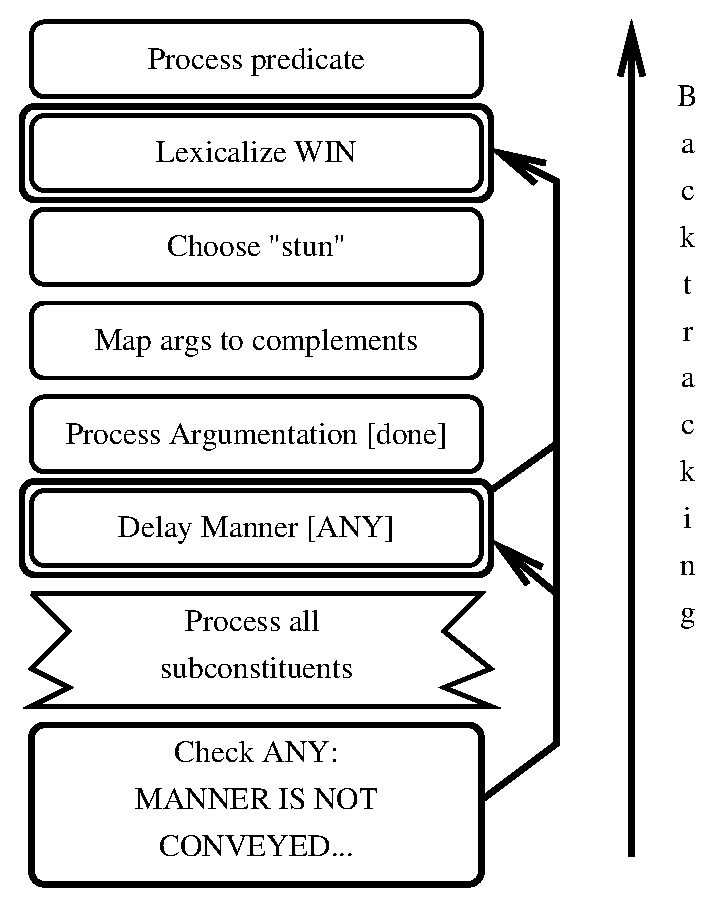
\includegraphics[width=4in, height=4in]{stack2.eps}
    \caption{Effect of bk-class}
    \label{fig4:floating-stack2}
\end{figure}

In general, the determination of the address of failure is more complex and
it is necessary to distinguish between {\em initial failures} and {\em derived
failures}.  An initial failure always occurs at a leaf of the total FD,
when trying to unify two incompatible atoms.  Failures, however, can also
propagate up the structure of the total FD.  For example, when unifying
{\tt ((a ((b 1))))} with {\tt ((a ((b 2))))} the original address of failure is
the path {\tt {a b}}. When the unifier backtracks, it also triggers a failure
at address {\tt {a}}, which is not a leaf.  This type of failure is called a
derived failure.  In the implementation of {\tt bk-class}, FUF ignores
derived failures and directly backtracks to the first choice point whose
{\tt bk-class} matches the last initial failure.  Determining whether a
failure is derived or initial can be difficult.  In FUF, the following
technique is used: I distinguish between {\em forward} and {\em backward}
processing.  Forward processing is the normal advance of the search
procedure through the disjunctions in the grammar.  Upon failure, backward
processing starts, which means that the stack of the last decisions is
unwound.  Each time a new disjunction is retried and restarted, forward
processing could restart, but unification may fail again immediately,
without making any changes to the total FD being processed.  In general,
backward mode continues until one of two events occurs: either a restarted
alt succeeds and at least one change is made to the total FD (a feature is
added to the input), or a failure occurs when unifying a grammar feature
with a feature that was present in the original input, before unification
started.  The distinction between forward and backward processing and the
way the address of failure is maintained is illustrated in Fig.\ref{fig4:bkclass1}.

%\pic{tag=fig4:bkclass1, file = bkclass1.ps, w=5in, h=3in, cap="Determination of the address of failure"}
\begin{figure}[p]
    \centering
    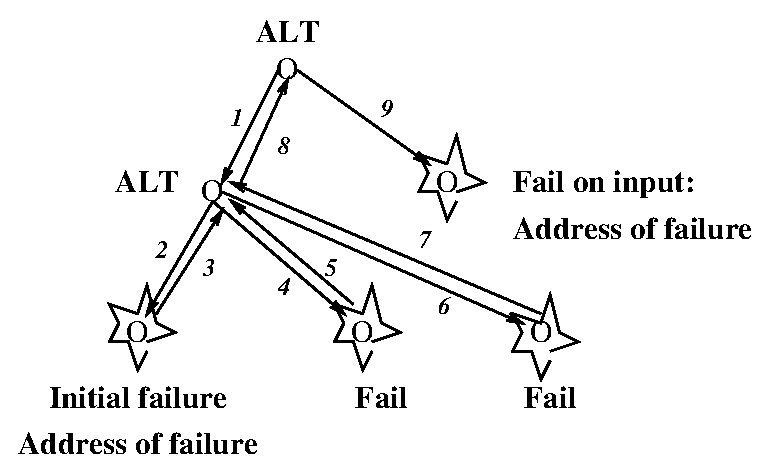
\includegraphics[width=5in, height=3in]{bkclass1.eps}
    \caption{Determination of the address of failure}
    \label{fig4:bkclass1}
\end{figure}

The figure shows the search space when traversing two successive alts in
the grammar.  Each arrow corresponds to either the choice of a branch in
the alt or to a forced backtracking.  Arrows 1 and 2 correspond to the
first forward processing step and end up in a failure.  This is an initial
failure and the {\em address of failure} (which is by definition the location
which caused the latest significant failure) is set to the current position
in the total FD.  The backward processing step starts and a second branch
of the ALT is tried (arcs 3 and 4).  This second branch fails immediately,
before any change is made to the total FD.  In such a case, the backward
processing step continues, and the address of failure is {\bf not} updated.
The motivation is that the unifier is still backtracking for the same
original reason: nothing changed in the grammar that makes the original
failure less relevant.  So the unifier keeps backtracking, and tries the
third and last branch of the ALT (arcs 5 and 6).  The same failure occurs
again, and backward processing proceeds.  The second ALT is exhausted and,
therefore, fails, and the second branch of the first ALT is tried in turn
(arcs 7, 8 and 9).  At this time, two reasons can trigger a switch of
failure address:
\begin{itemize}
\item Unification fails immediately, before any changes are made, but the failure
is due to the incompatibility of a feature of the grammar with a feature
that was originally present in the input before unification started.  In
such a case, the failure is not ``caused'' by the branch of processing that
led to the initial failure, it is caused by the grammar itself with the
original input, and would have had occurred even if no decisions had been
taken before.  So the failure address is switched to the current address.

\item Unification succeeds and at least one feature from the grammar is added to
the total FD.  Forward processing starts again.  Any future failure can be
caused by these new changes, and cannot therefore be attributed to the old
initial failure.  So the failure address is also switched to the current
address.
\end{itemize}

There is one more complication with the use of the address of failure as a
source of information on what decision caused the failure: as already
mentioned in Sect.\ref{relpath-ambiguity}, a given location in the total FD
can be accessed through several paths from the top of the total FD (since
an FD is not a tree but can be an arbitrary graph).  So several distinct
paths, with different labels can identify the location where the failure
occurred.  The intelligent backtracking component must decide which path
should be matched against the bk-class specifications.  The convention used
here is the same one used to disambiguate the up-arrow notation presented
in Sect.\ref{relpath-ambiguity}: the path used to identify the address of
failure is the path written in the grammar on the feature that caused the
failure.  The motivation is that the grammar writer uses the path that is
the most meaningful to access features, and that incidental conflations
along this path would not be as informative for backtracking purposes.
Another approach could have been to use all the path addresses that
identify a location and match them against all bk-class specifications.
But this approach would have imposed too much overhead on the regular
backtracking mechanism.

The bk-class mechanism works well in practice.  For the basketball example
discussed above, I have measured the number of backtracking points required
to generate different clauses conveying the same core content.  The
following table summarizes these measurements.\footnote{In this table, {\em DN}
abbreviates {\em Denver Nuggets} and {\em BC} abbreviates
{\em Boston Celtics}.}

\begin{center}
  \begin{tabular}{ | p{12cm} | r | r |}
	\hline
	Input / Output & w/o bk-class & w/ bk-class \\ 
    \hline \hline

	\parbox[t]{10cm}{
		No floating constraints:
		{\em The DN beat the BC}} & 110 & 110 \\ \hline

	\parbox[t]{10cm}{
		Manner in the verb:
		{\em The DN edged the BC}} & 110 & 110 \\ \hline

	\parbox[t]{10cm}{
		Manner as adverbial:
		{\em The DN narrowly beat the BC}} & over 10,000 & 214 \\ \hline

	\parbox[t]{10cm}{
		AO in the verb:
		{\em The DN stunned the BC}} & 112 & 112  \\ \hline

	\parbox[t]{10cm}{
		AO as adjective:
		{\em The hapless DN beat the BC}} & 1,623 & 239 \\ \hline

	\parbox[t]{10cm}{
		AO as adverbial:
		{\em The DN surprisingly beat the BC}} & over 100,000 & 268 \\ \hline

	\parbox[t]{10cm}{
		AO \& manner together:
		{\em The hapless DN edged the BC}} & 1,178 & 246 \\ \hline
    \hline
  \end{tabular}
\end{center}

The number of backtracking points required to generate each example clause
is listed with and without {\tt bk-class}.  The numbers for the first clause,
which does not include any floating constraints, give an indication of the
size of the grammar.  It roughly corresponds to the number of unretracted
decisions made by the grammar.  It is the optimal number of backtracking
points that a search control regime can obtain for the given input with
this grammar.  Without {\tt bk-class}, the wide variation in number of
backtracking points among the examples indicates the exponential nature of
the blind search which floating constraints impose on the standard control
regime.  In contrast, with {\tt bk-class}, the variation in number of
backtracking points remains within a factor of three among all the
examples.  



\section{Lazy Evaluation and Freeze with wait}

The {\tt bk-class} mechanism is useful in general to correct directly a
decision made a long time ago, as soon as it appears that the decision was
wrong.  But this implies that all the work done between the wrong decision
and the realization that it is wrong must be re-done once the original
wrong has been corrected.  For example, in the following case:

\begin{lstlisting}[language=Lisp]

Frame TOP  ---------> failure because of feature P
Frame T100 )
Frame T099 )
...        )----> Lots of decisions that do not 
...        )      affect the value of P.
...        )
Frame T016 )
Frame T015 ---------> feature P is set to wrong value
Frame T014
...
Frame T001 

\end{lstlisting}


The decisions corresponding to frames T016 to T100 are going to be done
twice because T015 made the wrong choice originally.  While making a
decision twice is not too bad compared to the cost of exhaustively
searching all the choices corresponding to frames T016 to T100 backwards,
it is still sub-optimal.

One could reach a more efficient solution if the decision corresponding to
frame T015 is delayed and the unifier commits to a value for P only after
frame T100.  The {\tt wait} control specification is used to achieve this
effect under certain conditions.

Wait specifies that the decision corresponding to a disjunction depends on
the value of certain features.  The syntax is as follows:

\begin{lstlisting}[language=Lisp]
(alt TP (:wait P) ...)
\end{lstlisting}

This declaration indicates to the unifier that the alt TP depends on the
value of the feature P.  If when it is first met feature P is instantiated,
then the alt is evaluated normally.  If however P is not yet instantiated,
the whole disjunction is delayed: it is put on hold, on an agenda.  The
rest of the grammar is evaluated, and periodically, the unifier checks the
agenda to determine if one of the frozen alts can be awakened.  

The following example illustrates a possible use of {\tt wait}:

\begin{lstlisting}[language=Lisp]

 ;; In conjunction: do verb ellipsis?
 ;; If the same verb is used in both conjuncts
 ;; you can ellide it in the second conjunct:
 ;; --> John ate the burger and Mary the fish.
 ;; The ellipsis is done by adding a GAP feature to the second verb.
 ;; Wait until verbs for both conjuncts have been selected. 
 ;; This alt does NOT determine what the verbs should be. 
 (alt verb-ellipsis (:wait {constituent1 process lex}
                           {constituent2 process lex})
   (((cat clause)
     ({^ constituent1 process lex} {^ ^ ^ ^ constituent2 process lex})
     ({^ constituent2 process gap} yes)
     (verbal-ellipsis yes))
    ((verbal-ellipsis no)))))

\end{lstlisting}


This fragment is extracted from grammar gr10.  It is part of the branch
of the grammar dealing with conjunction.  This alt implements the decision
whether to use a verb ellipsis in a conjunction of two clauses.  The verb
in the second conjunct can be elided if it the same lexical entry as the
verb in the first conjunct.  This match is checked by testing that the
{constituent1 process lex} path can be unified with the {constituent2
process lex} path.  When it can be unified, the {constituent2 process} is
enriched with the feature (gap yes), which the linearizer will interpret by
skipping the verb in the final sentence.

\index{constituent traversal}
Now remember that the standard control flow in FUF is top-down
breadth-first in the tree of constituents.  A conjunction of clauses is
made up of the following constituents:

\begin{lstlisting}[language=Lisp]
COMPLEX-CLAUSE
  |
  |---- ELEMENTS 
  |       |
  |       |--- CONSTITUENT1 
  |       |       |
  |       |       |--- PROCESS
  |       |       |--- PARTICIPANTS
  |       |       |--- SYNT-ROLES
  |       |
  |       |--- CONSTITUENT2
  |       |       |
  |       |       |--- PROCESS
  |       |       |--- PARTICIPANTS
  |       |       |--- SYNT-ROLES
  |       |       |
\end{lstlisting}

When the branch of the grammar specifying the conjunction is traversed, the
choice of the lexical item that will realize the process is still three
levels down.  The decision whether to use an ellipsis concerns only the
conjunction grammar, so it must be located in the conjunction branch, not
in the branch of the grammar deciding on lexical choice for the process.  
But it depends on this later decision - we do not want to influence the
choice of the verbs in the conjunct by the fact that they are conjoined.
So the decision is instead delayed until the verbs in both conjuncts have
been determined.  

Note that if the input already specifies the verbs, then the decision can
be evaluated right away.  It is only delayed when needed.

There can be complications when using {\tt wait} when two decisions wait for
each other, in a deadlock configuration.  I have not yet encountered such
situations in practice but in such cases, a combination of {\tt wait} and
{\tt bk-class} could ensure that the deadlock can be broken in an efficient
way.

\subsection{Wait and Constituent Traversal}
\label{wait-cset}
\index{constituent traversal}

The delaying of disjunctions interacts in a complex manner with the way the
constituent structure is traversed.  Recall that the traversal proceeds as
follows: the toplevel constituent is unified with the grammar, then at the
end of the unification (before determination time), the {\tt cset} of the
constituent is identified, and every descendant specified in the {\tt cset}
is traversed, in order.  The structure is then traversed breadth first.

As explained in Sect.\ref{incr-cset}, there are two ways to specify a
{\tt cset} in a constituent in FUF: implicitly and explicitly.  The
{\tt cset} is explicitly specified if there is a complete {\tt cset} feature
found in the constituent.  Otherwise it is implicit.  The implicit {\tt cset}
is found by using two heuristics: first it is assumed that any path
mentioned in a pattern is also a constituent; second, any feature which
contains a sub-feature of the form {\tt (cat xx)} is also assumed to be a
constituent.

To override these heuristics, the grammar writer can use {\em incremental
cset specifications}.  There are indeed two types of {\tt cset}
specifications: complete and incremental.  A complete specification is of
the form {\tt (cset (c1 ...  cn))} and exhaustively identifies all the
subconstituents of the current constituent.  An incremental specification
is of the form:
$(cset (+ a_{1} ... a_{m}) (- d_{1} ... d_{p}))$

An incremental {\tt cset} specifies that all the {\tt a\-{i}}s should be added
to the implicit {\tt cset} and all the {\tt d\-{j}}s should be removed from it.
The possibility of specifying the constituent structure incrementally is a
great convenience practically since it allows the grammar writer to give
partial information on constituency in different regions of the grammar.

Incremental cset specifications may affect delayed disjunctions.  The
following example illustrates this situation:

\begin{lstlisting}[language=Lisp]
((alt (:wait {^ manner conveyed})
  (((manner ((conveyed any)))
   ((manner ((conveyed adverb)
             (cat adverb) ...))
    (cset ((+ manner))))))))
\end{lstlisting}

In this case, the decision to express the manner constraint by using an
adverb is delayed, leaving a chance for the verb to express it as a
connotation.  Thus, in the first pass through the grammar, this alt is not
evaluated.  At the end of the processing of the clause constituent, the
cset is determined.  The implicit cset is computed and all the incremental
cset specifications are added on it.  At this point, the {\tt manner} feature
is not identified as a constituent, since there is no cat specified for it
and no incremental cset has added it explicitly.  The constituent structure
is then traversed.  At the end of this traversal, the delayed alts on the
agenda are processed.  The manner alt is thus unblocked, and the second
branch is eventually selected.  An adverb constituent is then added at the
clause level.  When the alt is completely processed, this adverb
constituent should be unified with the adverb grammar as any subconstituent
would be, if it had been processed without being delayed.  Unfortunately,
the constituent structure was already computed before the delayed alt was
unblocked.  And the adverb was not part of the cset at this time.  So the
adverb is not added to the final constituent structure of the clause.

\index{determination}
I have extended the determination process to re-check the constituent
structure whenever an alt has been unblocked during determination, thus
allowing new constituents to be added by delayed alts without restriction.
The determination process performs the following task: first, a delayed alt
is selected (the first one that was put on the agenda is chosen) and its
evaluation is forced.  Next, unification starts again to evaluate all the
delayed alts which have been unblocked by the evaluation of the forced alt.
At the end of this unification step, determination starts again.  This loop
continues until the agenda is empty.  At this point, the constituent
structure is recomputed and retraversed from the top of the total FD down,
in breadth-first order.  All constituents which have already been unified
are skipped, all new constituents identified by the recomputation of the
{\tt cset}s at the end of the agenda evaluation are unified again.  After
this unification step, determination starts again from scratch (since the
evaluation of the new constituents may have added delayed alts on the
agenda), until the agenda is empty and all constituents have been unified.

This top-down traversal in several passes integrates nicely the regular
top-down control regime with the benefits of the dynamic re-ordering of
constraints provided by {\tt wait}.  Note that this traversal in several
passes does not translate in reduced efficiency: it is only triggered when
needed (that is, when decisions had to be delayed), and the
traversal/recomputation of the constituent structure is a very efficient
operation.  As measured, efficiency is overall drastically improved with
{\tt wait}. 



\section{Conditional-Evaluation with Ignore}

The {\tt ignore} control annotation allows the grammar writer to evaluate
certain decisions only under certain conditions. The idea is to just ignore
certain decisions when there is not enough information, there is already
enough information or there is not enough resources left.  The 3 cases
correspond to the annotations:

\begin{lstlisting}[language=Lisp]

	(alt (:ignore-when <path> ...) ...)
	(alt (:ignore-unless <path> ...) ...)
	(alt (:ignore-after <number>) ...)

\end{lstlisting}

{\tt Ignore-when} is triggered when the paths listed in the annotation are
already instantiated.   It is used to check that the input already contains
information and the grammar does not have to re-derive it.

{\tt Ignore-unless} is triggered when a path is not instantiated.
It is used when the input does not contain enough information at all, and
the grammar can therefore just choose an arbitrary default.  A real
example of the use of {\tt ignore-unless} is given below. 

{\tt Ignore-after} is triggered after a certain number of backtracking points
have been consumed.  It indicates that the decision encoded by the
disjunction is a detail refinement that is not necessary to the completion
of the unification, but would just add to its appropriateness or value.
(IGNORE-AFTER IS NOT IMPLEMENTED IN FUF5.2).

\label{wait-ignore}
One characteristics of these annotations is that their evaluation may
depend on the order in which evaluation proceeds.  Since this order is not
known to the grammar writer, their use can be delicate.  To prevent
unpredictable variations, the {\tt ignore} annotations should be used in
conjunction with {\tt wait}, since {\tt wait} establishes constraints on when a
decision is evaluated.  Therefore a {\tt wait} annotation has priority over
an {\tt ignore} when both occur in the same alt.  Adding a {\tt wait}
annotation can often ensure that the {\tt ignore} annotation will only be
considered when it is relevant.

The following example is extracted from grammar gr10.  It is actually the
same case of verb ellipsis in conjunction presented in the section on
{\tt wait} above.  In this decision, we also want to specify that the whole
decision of whether to use ellipsis or not is only relevant in the case of
a conjunction of clauses.  This is expressed by addition the
{\tt ignore-unless} annotation as shown in the following figure:

\begin{lstlisting}[language=Lisp]

 ;; In conjunction: do verb ellipsis?
 ;; This decision ONLY applies to CLAUSEs.
 ;; Ignore it in conjunctions of NPs and other cats.
 (alt verb-ellipsis (:wait process)
   (:ignore-unless ((cat clause)))
   (((cat clause)
     ({^ constituent1 process lex} {^ ^ ^ ^ constituent2 process lex})
     ({^ constituent2 process gap} yes)
     (verbal-ellipsis yes))
    ((verbal-ellipsis no)))))

\end{lstlisting}


\chapter{Tracing and Debugging}
\index{tracing}

\section{What it Means to Debug a FUF Program}

When using FUF, a grammar developer is programming in the FUF programming
language.  The grammar is a program.  The input FD is the input to the
program.  FUF is the interpreter and sentences are the output of the
execution of a grammar on inputs.  In this framework, when something ``goes
wrong,'' the grammar developer must debug his grammar.  The main sources of
bugs found when developing FUF programs are:
\begin{itemize}
\item The input is not well formed (it is not a valid FD).

\item The grammar is not well formed (it is not a valid FD).

\item The input does not have the structure expected by the grammar (too flat or
too deeply nested).

\item The constituent structure is badly specified in the grammar (causing either
too many constituents to be generated, or not enough, or infinite recursion
in the constituent traversal).

\item The ordering patterns are not correctly specified or two pattern
specifications do not unify. 

\item The appropriate morphological features are not passed to the
leaf-constituents, preventing the morphology module from performing the
required inflections.

\item Relative paths are not pointing to the place they were intended to.
An ambiguous relative path is not correctly resolved.

\item Given/any fail when they should not: given can interact poorly with wait,
and should be replaced by any, any can cause heavy backtracking and should
be replaced by given.

\item Types are not defined as expected, or there is an unwanted interaction
between types. 

\item FSET declarations are too rigorous.

\item Wait and/or bk-class are not used correctly.

\item An indexed feature is not found in an indexed alt.
\end{itemize}

The main problem when debugging a FUF program is to identify what caused a
failure to occur.  We introduce the following terminology to discuss the
various debugging tools available in FUF: a failure occurs whenever the
unifier attempts to unify a simple leaf symbol with a different,
incompatible leaf.  Failures trigger backtracking.  An unexpected failure
is a failure that the programmer did not expect.  The initial failure is
the first unexpected failure to occur during an unification.  The
distinction between regular failure and unexpected failure is of course
subjective, but it is useful, because there are usually many failures that
occur even if there are no bugs in the grammar.  This happens whenever a
non-indexed alt is traversed.  Branches are tried in order until the
appropriate branch is found.  When failure occurs during the test of the
initial branches, this is not the trace that ``something is going wrong''.
So the main problem of the FUF debugger is to, as quickly as possible,
identify the initial failure - and to filter out all the irrelevant
expected failures.
\label{initial-failure}
\index{initial failure}

This task is made difficult because FUF backtracks a lot, and if the
initial failure is missed, a lot of subsequent ``unexpected failures'' will
occur when wrong branches are tried upon backtracking (in a sense,
everything that happens after the initial failure should be disregarded, as
the unifier is engaging on a wrong course).

This chapter presents the tracing tools available in FUF and provides
advice on how to use them to quickly identify the initial failure.


\section{Checking the Validity of FDs and Grammars}

Before tracing the unification, it is important to check that both the
input and the grammar are valid FDs.  The following functions perform this
checking: 

\begin{lstlisting}[language=Lisp]
(FD-SYNTAX fd)
;; check that a Lisp expression FD is a well-formed FD.

(FD-P fd)
;; check that a well-formed FD does not contain inconsistencies
;; (that is, (u fd nil) is not :fail, or in other terms, the FD
;; does not contain contradictory features, such as ((a 1) (a 2))).

(GRAMMAR-P grammar)
;; check that a Lisp expression grammar is a well-formed grammar.
\end{lstlisting}

When you suspect that your current input/grammar do not work, check first
that they are syntactically valid using these functions.


\section{Fine Tuning Tracing: Overview of FUF Tracing Functions}

Several dimensions characterize the activity of the FUF unifier:
\begin{itemize}
\item Where in the {\em input} is the unification proceeding.

\item Where in the {\em grammar} is the unification proceeding.

\item How {\em important} is the current action of the unifier.

\item What {\em stage} of the unification is proceeding.
\end{itemize}

It is possible to tailor the tracing behavior of FUF according to each of
these dimensions.  In general, FUF can output a tracing message whenever it
takes an action, such as adding a feature to the total FD, selecting a
branch in the grammar, backtracking because of a failure, expanding a cset
and moving in the constituent tree traversal, freezing and unfreezing
goals etc.  Outputting all the possible trace messages is always
overwhelming, and provides too much text to be useful.  So the challenge of
the FUF debugger is to fine-tune the tracing system to produce just enough
information to locate the bugs in the grammar and/or in the input FD.

The grammar developper indicates what portions of the grammar must be
traced: the grammar is traced, not the unifier. Therefore, to trigger
tracing, one must put directives into the grammar. At the Lisp level, and
for a given grammar including tracing directives, traces can be switched on
or off by the following functions:

\begin{lstlisting}[language=Lisp]
;; I GENERAL TRACING CONTROL

(trace-on)  ;; enable all trace messages to be output.
(trace-off) ;; disable all trace messages to be output
(trace-bp &optional (frequency 10))
	;; Output a dot for every frequency backtracking points.
	;; Useful for long computations to get a feeling of what's happening.
	;; Works even if (trace-off).
%break%	;; allows the insertion of break points in the grammar.
(trace-level level)
	;; Determines detail level of trace to be printed.  The following
	;; levels are defined:
    ;;                   00: feature level action
    ;;                   05: unimportant alt-level action
    ;;                   10: alt-level action - branch number trying
    ;;                   12: demo messages
    ;;                   15: freeze, ignore, bk-class
    ;;                   20: constituent level action
    ;;                   30: important failure - end of alt

;; II TRACING FLAGS MANAGEMENT: ENABLE \& DISABLE

(all-tracing-flags &optional (grammar *u-grammar*))
    ;; return the list of all tracing flags defined in grammar.
(trace-disable flag)  
	;; disable flag.  
	;; Everything works as if flag was not defined in the grammar.
(trace-enable flag)   ;; re-enable a disabled flag.
(trace-disable-all)   ;; disable all flags.
(trace-enable-all)    ;; re-enable all flags.
(trace-enable-alt alt-name :expansion t :grammar g)
(trace-disable-alt alt-name ...)
	  ;; Enable all tracing flags defined under a def-alt or
	  ;; def-conj.  If expansion is nil, does not expand the
	  ;; sub-def-alt. 
(trace-disable-match string)
	  ;; disable all flags whose names contain string.
(trace-enable-match  string)
	  ;; re-enable all flags whose names contain string.

;; III CONTROL OF SPECIFIC ACTIVITY TRACING

(trace-determine :on t|nil)  ;; enable tracing of determine stage or not.
(trace-category :all|cat|(cat1...catn) t|nil) 
	;; enable tracing of categories or not.
(trace-bk-class t|nil)  ;; list special messages concerning bk-class
(trace-wait :on t|nil)  ;; list special messages concerning goal freezing
(trace-cset :on t|nil)  ;; trace cset expansion
(trace-alts :on t|nil)  ;; detailed tracing of all alts, even unnamed.
(hyper-trace-category cat :status t|nil)
	;; trace category with printing of full constituent
	;; before unification of constituents of the traced cats.
\end{lstlisting}
\index{trace-on (function)}
\index{trace-off (function)}
\index{trace-level (function)}
\index{trace-bp (function)}
\index{all-tracing-flags (function)}
\index{trace-disable (function)}
\index{trace-enable (function)}
\index{trace-enable-all (function)}
\index{trace-disable-all (function)}
\index{trace-enable-alt (function)}
\index{trace-disable-alt (function)}
\index{trace-enable-match (function)}
\index{trace-disable-match (function)}
\index{trace-determine (function)}
\index{trace-category (function)}
\index{trace-bk-class (function)}
\index{\%break\%}
\index{trace-wait (function)}
\index{trace-cset (function)}
\index{trace-alts (function)}
\index{hyper-trace-category (function)}


\section{Identifying Possible Bugs: Trace-bp}

To identify whether FUF enters into unbounded backtracking (which is the
sign of a bug in the grammar or in the input), it is useful to first
monitor how many backtracking points are being used.  This can be achieved
by using the {\tt trace-bp} (trace backtracking points) function.  This is
the only tracing function which can be activated even if the general
tracing system is turned off (with the function {\tt trace-off}).  The effect
of the function is to output a dot on the screen every n backtracking
points, where n is 10 by default and can be changed by giving an argument
to {\tt trace-bp}.  The form of the function is:

\begin{lstlisting}[language=Lisp]
(TRACE-BP &optional n)

(TRACE-BP nil): turns off printing of .
\end{lstlisting}

If the string of dots becomes longer than expected, then it is worth
stopping the unifier under the suspicion that something is going wrong, and
to start the tracing system with {\tt trace-on}.

\section{Levels of Tracing}
\index{trace-level (function)}

In the attempt to reduce the amount of trace messages and finding the
original source of failure, the most useful tool is the {\tt trace-level}
function, which filters tracing messages according to their importance.
The following levels of importance are predefined:
\index{trace-level (function)}
\begin{itemize}
\item 30: important failure - end of alt

\item 20: constituent level action

\item 15: freeze, ignore, bk-class

\item 12: demo messages

\item 10: alt-level action - branch number trying

\item 05: unimportant alt-level action

\item 00: feature level action
\end{itemize}

The function {\tt trace-level} sets the minimum level of tracing messages
that can be printed.  Thus, calling (trace-level 20) insures that only
important messages of level 20 and 30 will be printed.

The levels are defined as follows:
\begin{itemize}
\item 30: An ``important'' failure in unification occurs - that is, all the
branches of an alt have been tried and failed.  This in general means that
the input is not compatible with the grammar.  It does not force immediate
failure of the overall unification process, because some backtracking
options may still be open, but it is a strong indication that something
wrong is going on.  In general, there is a high probability that the
{\em first} level 30 failure message is the initial failure (cf.
p.\pageref{initial-failure}). 

\item 20: Constituent Level Action - traces the constituent tree traversal of
FUF.  Whenever the grammar is re-accessed to unify a new constituent, a
tracing message is printed.  This is useful to follow the progression of
the unifier through the total FD.  In general, the traversal is a
top-down breadth-first expansion of the constituent tree.

\item 15: Control messages: The dominant control strategy of FUF is the top-down
constituent traversal.  Fine-tuning of this strategy is, however, possible,
using the {\tt bk-class}, {\tt wait} and {\tt ignore} directives.  These
constructs are described in more detail in Section \ref{control}.

\item 12: Demo messages: The alt construct allows the grammar writer to output
``demo messages'' when an alt is entered.  These messages are considered of
level 12.

\item 10: Alt-level action - branch number trying: when an alt is tried, branches
are tried successively, in order, randomly (for a ralt) or directly (for an
indexed alt).  A tracing message is output each time a branch is tried,
indicating the name of the alt (therefore the position of the unifier
within the grammar) and the number of the branch within the alt.

\item 05: unimportant alt-level action: when an alt is indexed, certain tracing
messages are printed to document the index search.

\item 00: feature level action: each time a feature is added to the total FD by
the unifier, a tracing message is printed.  This is the absolute lowest
level of tracing and results in unending seas of messages.
\end{itemize}

In general, when debugging, start by setting (trace-level 30), this 
provides most of the time directly the location of the initial failure. 


\section{Tracing of Alternatives and Options}
\index{tracing (of alt)}
\index{tracing (of opt)}
\index{alt (keyword)}
\index{opt (keyword)}

To follow the unifier as it proceeds through the grammar, the most useful
trace is generated by giving a name to an alternative of the grammar. It is
done by adding an atomic name after the keywords {\tt alt}, {\tt ralt} or
{\tt opt} in the grammar:

\begin{lstlisting}[language=Lisp]
((alt PASSIVE
 (
  ;; branch 1 of alt passive
  ((verb ((voice passive)))
   (prot none))
  
  ;; branch 2 of alt passive
  ((verb ((voice passive)))
   (prot any)
   (prot ((cat np)))
   (by-obj ((cat pp) (prep ((lex "by"))) (np (^ prot))))
   (pattern (dots verb by-obj dots)))))

 ;; body of alt passive (common to all branches)
 (verb ((cat verb-group))) 
...)
\end{lstlisting}

Here, this fraction of the grammar has been marked by the
directive: {\tt (alt PASSIVE ...)}. (An equivalent notation is {\tt (alt
(:trace PASSIVE) ...)}.)  The effect will be that all
unification done subsequently will be traced, producing the
following output:

\begin{lstlisting}[language=Lisp]
--> Entering ALT PASSIVE
--> Trying Branch #1 in ALT PASSIVE:
--> Fail on trying (prot none) with 
				   (prot ((nnp ((n ((lex boy)))))))
--> Trying Branch #2 in ALT PASSIVE:
        ...
\end{lstlisting}

If a traced alternative is found later in the grammar, the level of
indentation will increase. If the level of indentation decreases,
that means a whole {\tt (alt ...)} has failed. It is indicated by the output:
\index{failure (of unification)}

\begin{lstlisting}
--> Fail on ALT PROT.
\end{lstlisting}

The possible messages printed when the grammar is traced are:
\index{tracing messages}

\begin{lstlisting}[language=Lisp]
;; Move in the alternatives:
;;        ENTERING ALT f: BRANCH #i
;;        FAIL IN ALT f
;;        When the alt is indexed:
;;        ENTERING ALT f -- JUMP INDEXED TO BRANCH #i INDEX-NAME
;;        NO VALUE GIVEN IN INPUT FOR INDEX INDEX-NAME - NO JUMP
;; For options:
;;	TRYING WITH OPTION o
;;	TRYING WITHOUT OPTION o
;; Regular unification:
;;        ENRICHING INPUT WITH s AT LEVEL l
;;        FAIL IN TRYING s with s AT LEVEL l
;; Pattern unification:
;;        UNIFYING PATTERN p with p
;;        TRYING PATTERN p 
;;        ADDING CONSTRAINTS c
;;        FAIL ON PATTERN p
;; Unification between pointers to constituents:
;;        UPDATING s WITH VALUE s AT LEVEL l
;;        s BECOMES A POINTER TO s AT LEVEL l
;;        UPDATING BOTH PATHS TO A BOUND
\end{lstlisting}



\section{Local tracing with boundaries}
\index{tracing (local)}
\index{tracing flag}

If you want a more focused tracing, you can put anywhere in the grammar
a pair of atomic flags whose first character must be a "%" (value of
variable {\tt *trace-marker*}). All the unification done between the 2 flags
will be traced, and will produce the same messages as usual.
\index{\*trace-marker\* (variable)}

\begin{lstlisting}[language=Lisp]
	  ;; branch 2 of alt passive
	  ((verb ((voice passive)))
	   (prot any)
	   %by-obj%
	   (prot ((cat np)))
	   (by-obj ((cat pp) (prep ((lex "by"))) (np (^ prot))))
	   %by-obj%
	   (pattern (dots verb by-obj dots)))
           ...
\end{lstlisting}

All the unification done between the 2 flags %by-obj% will be traced.
You furthermore will have a message:

\begin{lstlisting}[language=Lisp]
Switching local trace flags on and off:
        TRACING FLAG f
        UNTRACING FLAG f
\end{lstlisting}

You generally want to have only small portions of the grammar put between
tracing flags.

\subsection{Special Flags \%trace-on\% and \%trace-off\%}

The special tracing flags {\tt \%trace-on\%} and {\tt \%trace-off\%} are predefined
and have the effect of temporarily turning all tracing on and off.  They
are used as all other local tracing flags, as shown in the following
example:

\begin{lstlisting}[language=Lisp]

       ((alt PASSIVE
	 (
	  ;; branch 1 of alt passive
	  ((verb ((voice passive)))
	   (prot none))
	  
	  ;; branch 2 of alt passive
	  ((verb ((voice passive)))

	   %trace-off%          ;; Turn off tracing of details in this branch

	   (prot any)
	   (prot ((cat np)))
	   (by-obj ((cat pp) (prep ((lex "by"))) (np (^ prot))))
	   (pattern (dots verb by-obj dots))

	   %trace-on%           ;; Turn tracing back on

	   )))

	;; body of alt passive (common to all branches)
	(verb ((cat verb-group)))
	...)

\end{lstlisting}

{\tt \%Trace-off\%} is generally used to remove tracing information from
a region of the grammar that has already been debugged but still leaving
the alt traversal tracing messages on.  The same effect is most of the
time achieved by using the {\tt trace-level} function, but {\tt \%trace-off\%}
allows finer tuning of the tracing behavior of FUF.


\subsection{The Special Tracing Flag \%break\%}

The special tracing flag {\tt \%break\%} is used to trigger a break in the
execution of FUF.  When found by FUF, a Lisp continuable break is
triggered.  It is then possible to examine the current state of the
unification using the Lisp debugger.  Using the Lisp debugger, it is then
possible to either resume unification or abort it.  Within the debugger,
the total fd can be inspected (and modified) by using the function
{\tt path-value} and {\tt set-path-value}.  A typical session is shown below:

\begin{lstlisting}[language=Lisp]

(setq *u-grammar* 
	'((alt (
		((cat clause) (pattern (s v o))
		 (s ((cat np)))
		 (v ((cat v)))
		 (o ((cat np))))
		((cat np) %break%)
		((cat v) %break%)))))

;; The np and v branch are not yet written - a break is inserted
;; The developer can then insert new values manually during unification.

LISP> (uni '((cat clause) 
             (s ((lex "John"))) 
             (v ((lex "like"))) 
             (o ((lex "Mary")))))

>========================================
>STARTING CAT CLAUSE AT LEVEL {}
>========================================
>Expanding constituent {} into cset ({O} {V} {S}).
>

>========================================
>STARTING CAT NP AT LEVEL {O}
>========================================

Break: Break in grammar

Restart actions (select using :continue):
 0: return from break.
{1c} FUG5 23> (path-value {o})

((LEX "Mary") (CAT NP)) 
{1c} FUG5 24> (path-value {n})

((LEX "John") (CAT NP))

{1c} FUG5 25> :cont

>Constituent {O} is a leaf.
>

>========================================
>STARTING CAT V AT LEVEL {V}
>========================================
Break: Break in grammar

Restart actions (select using :continue):
 0: return from break.
{1c} FUG5 26> :reset

FUG5 27> 
\end{lstlisting}

The behavior of the debugger depends on which version of Common Lisp you
are using.  The example shown here is run under Franz Inc's Allegro Common
Lisp.  Consult your Lisp manual to find out the details of how to resume
processing (the :cont command in ACL) and abort processing (the :res
command in ACL).  Another source of variation is whether the {} notation is
recognized within the debugger or not.  This notation is implemented using
macro characters in Lisp.  Macro-characters are recognized in ACL's
debugger but not in Lucid Common Lisp's implementation.  For that reason,
the function path-value accepts as parameter either a path or simply a
list of attributes.
\index{path-value (function)}

The function {\tt path-value} returns the value of a path in the current total
FD.  It is useful to inspect the current value of the total FD.  The
function {\tt set-path-value} is also defined to change a value within the
total FD.  Note that it's use is highly dangerous.

\begin{lstlisting}[language=Lisp]
(path-value path-or-list)  Return the value of path in the current total FD.

(set-path-value path-or-list FD)  Set the value of a path in the current 
			          total FD to FD.  

;; Examples:

(path-value {process v})
(path-value '(process v))  ;; equivalent form when the {} notation is not
                           ;; recognized 

(set-path-value {process v} '((lex "take")))

(set-path-value {process v} (u (path-value {process v}) '((tense past))))
                           ;; u performs a simple unification between fds.

\end{lstlisting}
\index{set-path-value (function)}

 
For more general access, the total FD is accessible in the special variable
{\tt *input*} and it can be modified in any possible ways.  But if you do
follow this way, there is a high probability that the unification will not
be able to proceed normally.  Note that there is no way to easily remove a
conflation from the total FD using only {\tt path-value} and {\tt set-path-value}
because {\tt path-value} always follows the paths until a non-path value can
be returned.  The following example illustrates this limitation:

\begin{lstlisting}[language=Lisp] 
(setq *input* '((a {b})
                (b ((b1 1)))))

(path-value {a}) --> ((b1 1))

(set-path-value {a} '((b1 2)))

(path-value {}) --> ((a {b}) (b ((b1 2))))

;; Cannot just with path-value and set-path-value remove the conflation
;; between a and b (a {b}).
\end{lstlisting}

One last word of caution: when using {\tt set-path-value}, relative paths are
made absolute before being inserted relative to the path of insertion given
as parameter.  Since the relative path notation can be ambiguous (cf
p.\pageref{relpath-ambiguity}), this can, under circumstances where there
is an ambiguity, create unexpected results.  


\section{The trace-enable and trace-disable Family of Functions}

\index{all-tracing-flags (function)}
\index{trace-disable (function)}
\index{trace-enable (function)}
\index{trace-enable-all (function)}
\index{trace-disable-all (function)}
\index{trace-enable-match (function)}
\index{trace-disable-match (function)}
\index{trace-enable-alt (function)}
\index{trace-disable-alt (function)}

In general, a grammar is defined in a file, that you load in your Lisp
environment.  The tracing flags are defined in that file after the alts and
opts or as local flags.  When you develop a grammar, you want to focus on
different parts of the grammar.  In order to do that, you can selectively
enable or disable some of the flags defined in the grammar.  

The function {\tt all-tracing-flags} returns a list of all the flags defined
in the grammar.  You can then choose to enable or disable all the flags,
only a given flag, or all flags whose name matches a given string.  

When a flag is disabled, everything happens as if the flag was not defined
at all in the grammar.  Note that you cannot create a new flag in the
grammar by using these functions.  You can simply turn on and off existing
flags.  It is therefore a good idea to define all the possible flags in a
grammar and to adjust the list of enabled flags from within lisp.

When you use the {\tt def-alt} and {\tt def-conj} notation (cf. Section
\ref{def-alt}), the functions {\tt trace-enable-alt} and
{\tt trace-disable-alt} can be used to enable and disable all the tracing
flags appearing under a given def-alt or def-conj construct.  The
{\tt expansion} keyword determines if the enabling/disabling only concerns
the tracing flags appearing directly in the def-alt construct, or also all
the flags appearing in the expansion of the construct.



\section{The :demo directive}
\index{demo (annotation)}

Reading traces from the unifier is a particularly tedious task.  The main
problem is that the messages generated by the program are very similar to
each other.  The {\tt :demo	} directive allows the grammar writer to bring
some variety to these messages.  A demo-message can be used to output a
specific message during the trace of the program when entering an alt (or a
ralt) construct.  The syntax is indicated by the following figure:

\begin{lstlisting}[language=Lisp]
      (alt voice (:demo "Is the voice active or passive?")
	   (((voice active)
             ...)
	    ((voice passive)
             ...)))
\end{lstlisting}

The message will be printed in the trace of the program (only if the
tracing flag voice is enabled) as shown:

\begin{lstlisting}[language=Lisp]

--> Entering alt VOICE
    Is the voice active or passive?
--> Trying branch #1 
    ...
\end{lstlisting}

Note that the message is indented in the stream of trace messages.  Such
messages allow the grammar writer to put some semantic information into the
trace messages, so that the whole stream of messages can be more easily
interpreted.  

In addition to its position at the top of an {\tt alt} construct, a
demo-message can be embedded anywhere in a grammar by using the
{\tt control-demo} function.  {\tt Control-demo} must be used within a
{\tt control} pair and produces an indented demo message in the trace stream.
The following example illustrates its use:
{\tt control-demo} \index{control-demo (function)}

\begin{lstlisting}[language=Lisp]
      (alt from-loc (:demo "Is there a from-loc role?")
	   (((from-loc none)
	     %TRACE-OFF%
	     (control (control-demo "No from-loc"))
	     %TRACE-ON%)
	    ((from-loc given)
	     %TRACE-OFF%
	     (control (control-demo "From-loc is here"))
	     %TRACE-ON%)))

;; Tracing output:

--> Entering alt FROM-LOC
    Is there a from-loc role?
--> Fail with branch #1
--> Entering branch #2
    From-loc is here
--> Success with branch #2

\end{lstlisting}

NOTE: The {\tt control} pair containing a {\tt control-demo} call should be put
within a \%TRACE-OFF\% - \%TRACE-ON\% pair to avoid the printing of system
trace messages regarding the control pair.

NOTE: The demo message string is passed to the {\tt format} common-lisp
function, and can therefore contain formatting characters accepted by that
function ({\em e.g.}, \~{} or \~{}\%).  Refer to your CommonLisp manual for details.



\section{Tracing of Specific Stages of the Unification}

The following group of function enable or disable tracing of specific
stages of the unification process:

\begin{lstlisting}[language=Lisp]
(trace-determine :on t|nil) 
(trace-category :all|cat|(cat1...catn) t|nil)
(trace-bk-class t|nil)  
(trace-wait :on t|nil)
(trace-cset :on t|nil)
(trace-alts :on t|nil)
(hyper-trace-category cat :status t|nil)
\end{lstlisting}

\subsection{Trace-determine}
\index{determination}
\index{trace-determine (function)}

The determination stage checks that no ANY constraint is left unsatisfied
at the end of the unification stage, and that all TEST constraints are
satisfied.  In addition, it checks that no further CSET traversal is
required to restore after frozen constraints have been thawed or forced.

When trace-determine is on, these checks generate tracing messages.  The
specific messages are:

\begin{lstlisting}[language=Lisp]

FAIL: Found an ANY at level <path>
Current Sentence: ....

TEST succeeds: <expr> at level <path>

Fail in testing <expr> at level <path>
\end{lstlisting}

The current sentence is only printed when FUF is called from the toplevel
function {\tt uni} whose function is to print a sentence.  In other uses of
FUF, the current function is not generated.  This message is of level 30
(highest level).

In addition, each time the determination stage is reached, a line of
statistics on backtracking is printed, of the form:

\begin{lstlisting}[language=Lisp]

{Used 119 backtracking points - 26 wrong branches - 15 undos}

\end{lstlisting}

Three pieces of information are provided: 
\begin{enumerate}
\item The total number of backtracking points used so far.  This can be
interpreted as the number of ``questions'' FUF asked to the grammar, or how
many times a branch had to be chosen in an alt construct.

\item The number of ``wrong branches'' - that is, how many times FUF picked up a
branch and started unification to finally undo this branch upon
backtracking.  This can be interpreted as the number of ``wrong guesses''
made by FUF.  

\item The number of ``undos'' - that is, how many features were added to the
total FD while traversing ``wrong guesses'' and were later removed from the
total FD upon backtracking.  This gives an indication of how ``deep'' FUF
went into wrong branches before realizing that they led to failure.
\end{enumerate}

When, because of the interaction between wait and the constituent traversal
(cf Section \ref{wait-cset}) a new cycle of unification must be started
after determination, a new line of statistics will be printed.  
\index{constituent traversal} 
These lines of statistics are NOT printed if the keyword parameter
{\tt non-interactive} is set to true when calling the top-level functions of
FUF (for example, as in {\tt (uni fd1 :non-interactive t)}).
\index{non-interactive (keyword)}

These statistic lines are printed indicate whenever a unification cycle
ends and a determination cycle starts.  They therefore provide important
information on how unification is proceeding.


\subsection{Trace-Category and Hyper-trace-category}
\index{trace-category (function)}
\index{hyper-trace-category (function)}
\index{constituent traversal}

Trace-category is useful to follow the traversal of the constituent
structure as it is performed by FUF. When a category C is traced, the
following message is printed whenever a constituent of category C is
unified with the grammar: 

\begin{lstlisting}[language=Lisp]
>========================================
>STARTING CAT ADJ AT LEVEL {SYNT-ROLES SUBJ-COMP HEAD}
>========================================

\end{lstlisting}

The function {\tt hyper-trace-category} provides more detail: if category C
is ``hyper-traced'', the same message is printed, and in addition the whole
constituent is printed:

\begin{lstlisting}[language=Lisp]
>========================================
>STARTING CAT ADJ AT LEVEL {SYNT-ROLES SUBJ-COMP HEAD}
>========================================

>CONSTITUENT {SYNT-ROLES SUBJ-COMP HEAD} =
((CAT ADJ) (CONCEPT {SYNT-ROLES SUBJ-COMP CONCEPT})
 (POLARITY {SYNT-ROLES SUBJ-COMP POLARITY})
 (LEX {SYNT-ROLES SUBJ-COMP LEX}))
\end{lstlisting}

The functions are used as follows:
\begin{lstlisting}[language=Lisp]
(TRACE-CATEGORY c | :all | (c1 ... cn)  &optional t | nil)
(HYPER-TRACE-CATEGORY c | :all | (c1 ... cn) &optional t | nil)
		Trace or hyper-trace a given category, or all categories
		(if parameter is :all) or a list of categories.
		If a second parameter nil is added, the category or 
		categories are untraced.
\end{lstlisting}


\subsection{Trace-Cset}
\index{trace-cset (function)}
\index{cset (keyword)}
\index{constituent traversal}


The {\tt trace-cset} function is used to monitor constituent traversal.  Each
time FUF finishes unifying a constituent, it computes the cset of the
result of the unification, applying the rules described in Section
\ref{cset-expansion}.  The constituents are then traversed breadth-first.
The function trace-cset triggers messages of the following form at the end
of the unification of each constituent:

\begin{lstlisting}[language=Lisp]

>Expanding constituent {} into cset ({SYNT-ROLES SUBJ-COMP}
                                     {PROCESS}
                                     {SYNT-ROLES SUBJECT}).
>

>========================================
>STARTING CAT AP AT LEVEL {SYNT-ROLES SUBJ-COMP}
>========================================

\end{lstlisting}

If the constituent has an empty cset, it means it is a leaf in the
constituent structure.  In that case, the following message is printed:

\begin{lstlisting}[language=Lisp]

>Constituent {SYNT-ROLES SUBJ-COMP HEAD} is a leaf.
>Constituent {PROCESS EVENT} is a leaf.
>

\end{lstlisting}


\subsection{Trace-BK-Class}
\index{trace-bk-class (function)}
\index{bk-class (annotation)}
\index{control in FUF}

The interpretation of the BK-class annotation has been introduced in
Section \ref{bk-class}.  BK-class is used to allow intelligent
dependency-directed backtracking.  Each choice point can be marked to
belong to a certain backtracking class (bk-class), and certain classes of
paths can be declared to belong to corresponding bk-classes.  Upon failure,
the address of failure is checked.  If it does not belong to a declared
bk-class, regular chronological backtracking is started.  If it does belong
to a bk-class, then backtracking continues up to the latest choice points
that belong to the same bk-class.

When tracing this behavior, the following conditions are monitored: (1)
when a special failure address is met and how high up the intelligent
backtracking progresses and (2) what is the latest address of failure.  
The following messages are printed in each case:

\begin{lstlisting}[language=Lisp]
>BK: Special path <path> caught by alt <alt> of class <c> after <n> frames.

>BK: Switch from <path1> to <path2>
\end{lstlisting}

The first message is emitted whenever intelligent backtracking occurs.  The
second one is emitted whenever the current address of failure is modified
following the rules discussed on page \pageref{fig4:bkclass1}.



\subsection{Trace-Wait}
\index{trace-wait (function)}
\index{wait (annotation)}
\index{control in FUF}


The wait annotation is used to allow goal delaying during the evaluation of
a grammar.  The idea is to wait until enough information is available
before trying to choose between the branches of an alt.  The grammar writer
indicates which information is requested before the evaluation of an
alt can start using the wait annotation and a sequence of path expressions
which point to the features which must be instantiated with the requested
information.  

When enough information is already present, the alt is evaluated as usual.
When there is missing information (some of the features are not yet
instantiated), the alt is frozen (delayed).  Frozen alts are stored on an
agenda, which keeps track of the decisions which remain to be made in the
future.  At regular intervals (in FUF, whenever a new choice point is met),
the agenda is checked, and if enough information has been gathered since
the time a decision has been frozen, the decision is thawed, and evaluated
immediately.  After the evaluation of the thawed alt, control proceeds
where it was interrupted.

In addition, at the end of the unification stage, the determination stage
checks if any decision is still on the agenda.  Such a situation is reached
if not enough information could be gathered anyway to allow the evaluation
of the frozen alts.  In this case, the frozen alts of the agenda are
``forced'' and evaluated, even though some of the requested information is
missing.  

Finally, there is one more configuration of control decisions which
concerns the goal delaying behavior of FUF:  as explained on page
\pageref{wait-ignore}, wait annotations have priority over ignore
annotations to insure that ignore annotations are only considered when
enough information is available for them to make sense.  When thawing a
frozen alt from the agenda, after enough information has been gathered, the
ignore annotations are immediately checked.  If they do match, then the
whole frozen alt is immediately ignored.

Corresponding to each of these configurations, the trace system emits the
following messages.  In every case, a unique agenda identifier (integer
number) is assigned to each frozen alt:

\begin{lstlisting}[language=Lisp]

>Freezing alt <alt>: waiting for <path> {agenda <n>}

>Thawing {agenda <n>}: Restarting at level <path>

>Forcing {agenda <n>}: Restarting at level <path>

>Ignoring {agenda <n>}

\end{lstlisting}


\subsection{Trace-Alts}
\index{trace-alts (function)}
\index{alt (special attribute)}

The function {\tt trace-alts} systematically monitors traversing of alts in
the grammar, even if the alts are not traced, and outputs a message
whenever a new branch is tried.  It is best used in conjunction with a
trace-disable-all setting, to follow uniquely alt traversal.  The form of
the output is as follows:
 
\begin{lstlisting}[language=Lisp]

LISP> (trace-disable-all)
LISP> (trace-alts)
LISP> (uni t1)

>========================================
>STARTING CAT CLAUSE AT LEVEL {}
>========================================

>Fail in alt VOICE
>Fail in alt VOICE-NORMAL
>Fail in alt VOICE-NORMAL
>Fail in alt VOICE-NORMAL
>Fail in alt DATIVE-MOVE-DEFAULT
>Fail in alt DATIVE-MOVE-DEFAULT
>Fail in alt SUBJECT-SUBCAT
>Fail in alt SUBJ-COMP-CAT
>Fail in alt :ANONYMOUS
>Fail in alt :ANONYMOUS
>Expanding constituent {} into cset ({SYNT-ROLES SUBJ-COMP}
                                     {PROCESS}
                                     {SYNT-ROLES SUBJECT}).
>
\end{lstlisting}

Each time a branch in an alt fails, the message ``fail in alt X'' is
printed.  If the alt is not traced, the name {\tt :anonymous} is printed
instead.  This is useful to find possible errors even in places which are
not traced in the grammar.  In general, {\tt trace-alt} should only be used
in last recourse.


\section{Some Advice on FUF Debugging}

This section provides some pragmatic advice on how to use the tracing
system of FUF based on the experience gathered while developing large
grammars.  It lists common sources of confusion, warns against the
misfeatures of the tracing system, common bugs and some successful bug
tracking tricks.


\subsection{Syntax Errors}

The first source of bugs, often incomprehensible ones, is syntax errors,
either in the input FD or in the grammar.  So the first precaution is to
check both inputs and grammars regularly.  Use functions FD-P and GRAMMAR-P
for that purpose.  In grammars, check especially the number of parentheses
occuring after ALTs.
\index{fd-p (function)}
\index{grammar-p (function)}

\subsection{Semantic Errors}

Semantic errors in the grammar can be trivial typos or the sign of a bad
design of the FD structure.  In any case check the following points:

\begin{itemize}
\item Mispellings: wrong feature-name, wrong leaf-value-name

\item Paths: in both forms, {\em i.e.}, {\tt ((f1 ((f2 ((f3} and {\tt \{f1 f2 f3\}}.  Make
sure that paths actually point to the location in the total FD that you
expect.  

\item The most common source of error is to include the wrong number of up-arrows
\^{} in a path expression.  Always double-check your relative paths,
especially those appearing embedded in ALTs, CONTROL, EXTERNAL when the
up-arrow notation can be quite counter-intuitive.
\index{relative path}
\index{\^{}n notation}

\item Observe the structure of the unified graph before unification.  To this
end, use the function {\tt uni-fd} and pretty-print its output as in:
\begin{lstlisting}
(pprint (clean-fd (uni-fd input :grammar gr)))
\end{lstlisting}
This is often instructive.  Use the function top-gdp to explore this output
FD in detail.
\index{top-gdp (function)}
\index{uni-fd (function)}
\index{clean-fd (function)}

\item Draw a graph of the total FD with all features instantiated to help you
check all your paths and levels of embedding.
\index{graph (FD as)}

\item If you do not understand the current structure of the FD, insert a \%break\%
in your grammar at some critical point, and use the function {\tt path-value}
to inspect the total FD during the time of the unification.
\index{ \%break\% }
\index{path-value (function)}

\item It is risky to use absolute paths in general (SURGE does not include a
single absolute path for example).  Using an absolute path is a sign of
desperation. 
\index{desperation (when debugging FUF)}
\index{absolute path}
\end{itemize}


\subsection{Expression of Negative Constraints}

Negative constraints are used to limit the scope of acceptable FDs by the
grammar and to force failure when certain FD configurations are met.  The
main tools in FUF for the expression of negative constraints are FSET and
NONE.  The main sources of confusion here are:
\begin{itemize}
\item FSET is too restrictive: you didn't plan on adding a feature, a new feature
is not compatible with FSET.  
\index{fset (special attribute)}

\item FSET must include explicitly all the features, including CAT and CSET.

\item NONE is used in the wrong place.
\index{none (special value)}
\end{itemize}


\subsection{Control}

The overall flow of control of FUF is quite complex, and the trace messages
do not make it very easy to follow.  Before going on and suffering
through the zillions of lines produced by the trace system, try to
understand analytically what could go wrong - recheck the syntax of
your fd and grammar, and recheck the structure of your FD and the structure
your grammar builds.  Only when this fails should you try to read the trace
messages to understand what went wrong on a particular input.  You should
proceed in the following order:
\begin{enumerate}
\item Identify that there is a bug: do (trace-off) and (trace-bp).  This will
emit a dot every 10 backtracking points (10 is the default) and indicate
how much effort FUF has invested on your input.  For example, when dealing
with SURGE, a clause that takes more than 300 backtracking points (30 dots
on the screen) is either very complicated or contains a bug.  When you
think there is a bug, interrupt the unifier (generally use control-C).
\index{trace-bp (function)}
\index{trace-off (function)}

\item Monitor the speed of appearance of the dots.  In general, FUF operates in
two modes: ``forward'' and ``backward''.  Forward mode is when the grammar
is traversed as expected, and every new feature falls into place.  Backward
mode is after the occurrence of the first unexpected failure.  The unifier
starts backtracking and tries every other branch in an unexpected manner.
In general, these tried branches fail very quickly.  So in backward mode,
backtracking dots tend to be emitted much more quickly than in forward
mode.  When the dots start piling up, it's a good sign that FUF has entered
backward mode, and that a bug has been found.

\item Once you suspect there is a bug, identify the first unexpected failure.
The first attempt to do that is to set (trace-on) and (trace-level 30).
This will print the most obvious candidates.  If this does not work,
basically, you're in trouble, and finding the bug will take time (sorry!
I'm in the middle of the implementation of a graphical debugger for FUF
which should help you beyond this stage).
\index{trace-on (function)}
\index{trace-level (function)}
\index{desperation (when debugging FUF)}

\item The next step is to gradually lower the trace-level until you get a good
understanding of where in the grammar is the source of the bug - moving to
values 20, 15, 12, 10, 5 and 0 (trying trace-level 0 on a full grammar
without disabling most of the tracing flags is a sign of desperation).
\index{desperation (when debugging FUF)}

\item Once the approximate location of the problem is identified in the grammar,
enable only the relevant tracing flags (those defined in the grammar around
the problematic spot).  This is achieved by using the functions
(trace-disable-all) (trace-enable-alt name-of-suspected-alt). 
\index{trace-disable-all (function)}
\index{trace-enable-alt (function)}

\item From then on, try to understand what's happening.  I find it convenient to
run FUF within an Emacs buffer and to use the editor to search through the
trace messages printed by FUF.
\index{EMACS (text editor)}

\item If you enable all tracing flags and set trace-level to 0 and you still
cannot find a tracing message identifying a failure (of the form ``FAIL in
...'') this can be due to 2 problems:
	\begin{enumerate}
	\item Either the failure is occurring in a region of the grammar which
	does not contain tracing flags.  In this case, set (trace-alts) and
	check the messages ``fail in alt :anonymous''.  
	\index{trace-alts (function)}
	\index{anonymous}

	\item Or the failure is due to a missing cat in the grammar.  Often if
	you unify ((cat xxx)) with a grammar that has no branch for xxx, 
	there is no failure message produced.  Check your cats often.
	\index{cat (special attribute)}
	\end{enumerate}
\end{enumerate}

The main points you should be looking for when debugging are:
\begin{itemize}
\item Endless backtracking: this can be found by setting trace-level 00 and
looking for repetition in the flow of messages.

\item Failure on ANY (especially in conjunction with recursion).
\index{any (special value)}

Failure on given (especially in conjunction with wait): remember that an
alt that is annotated with (wait path1) can be forced and therefore
evaluated even if path1 is not yet instantiated.  Therefore, using (path1
given) in such a situation is dangerous.  In this case, switch to any.
\index{given (special value)}
\index{wait (annotation)}

INDEX (especially double indexes and partial indexes).  Do NOT factor
together branches in an indexed alt.  For example, the following index will
not work (unification with ((a 1)) will fail):
\begin{lstlisting}
(alt (:index a)
  (((a ((alt (1 2)))))
   ((a 3))))
\end{lstlisting}
\index{index (annotation)}

WAIT (especially in conjunction with ignore and bk-class)

BK-CLASS: especially, since the bk-class declarations are persistent, do
not forget to evaluate (clear-bk-class) when loading a new grammar.  In
case of doubt, evaluate (clear-bk-class) and re-evaluate all your
(define-bk-class).  In general, it is good to add the following prelude in
all the files containing a grammar definition:
\begin{lstlisting}
(eval-when (load eval)
  (clear-bk-class)
  (reset-typed-features))
\end{lstlisting}
\index{clear-bk-class (function)}
\index{reset-typed-features (function)}
\index{bk-class (annotation)}

IGNORE: check that you do not ignore alts too liberally.
\index{ignore (annotation)} 

Constituent Structure Definition:
\begin{itemize}
\item Wrong cset (especially interaction between cat and explicit cset).  In case
of doubts, use an explicit cset in your grammar.  Avoid over-restrictive
csets (with the = notation), they often cause failure of unification with
further cset features in the grammar.

\item Wrong pattern and interaction between pattern and cset when using implicit
cset expansion.

\item Csets can trigger infinite recursion.
\end{itemize}
\index{cset (special attribute)}
\index{constituent traversal}

Linearizer: The linearizer produces strings of the form ``unknown cat: XXX''
when a category unknown to the morphology module is found as a leaf in the
constituent tree.  This is often due to the following effect: all top-level
unification functions have a :limit keyword option used to limit the number
of backtracking point used on a single input.  The default value for limit
is 10,000.  When unification stops after reaching this limit, the FD is
sent to the linearizer, even though it has not been completely unified, and
all constituents have not been completely expanded.  In that case, you can
get strings such as ``unknown cat: NP'' because an NP has not been expanded.
To correct this problem, increase the limit.
\index{linearizer} 
\index{limit (keyword)}
\index{unknown category}

Type Hierarchy Problems:
\begin{itemize}
\item Since the type declarations are persistent, do not forget to evaluate
(reset-typed-features) when loading a new grammar.  In case of doubt, use
{\tt draw-types} to verify the current state of type definitions.  In
general, it is good to add the following prelude in all the files
containing a grammar definition:
\begin{lstlisting}
(eval-when (load eval)
  (clear-bk-class)
  (reset-typed-features))
\end{lstlisting}
\index{clear-bk-class (function)}
\index{reset-typed-features (function)}
\index{draw-types (function)}

\item Wrong {\tt under} specification.
 
\item Wrong {\tt define-feature-type}

\item Lack of {\tt under} (when one wants only to test for the presence of a
feature and not to enrich the total FD).
\end{itemize}
\index{define-feature-type (function)}
\index{under (special value)}

\item Procedural types, test and control:
\begin{itemize}
\item Wrong CONTROL/TEST function

\item TEST for CONTROL and vice-versa.

\item Wrong use of the path construct with a TEST/CONTROL (with the \#\ notation).

\item Wrong EXTERNAL function.

\item Wrong procedural-type definitions.
\end{itemize}
\end{itemize}
\index{test (keyword)}
\index{external (keyword)}
\index{control (keyword)}
\index{pound notation} 
\index{define-procedural-type (function)}


\chapter{Manipulation of FDs as Data-structures}

FDs can be viewed as a convenient data-structure.  FUF provides a library
of Lisp functions to manipulate FDs: accessors to extract a sub-fd from a
total fd, insertion of an FD within a total FD, etc.  These functions' main
complexity lies in the interpretation of paths.  For example, if you want
to extract a sub-fd from a total fd, and this sub-fd contains path pointing
outside the sub-fd up into the total fd, the extraction function should
also extract these paths.  In addition, relative paths in the sub-fd must
be adjusted to maintain consistency.  

Another class of functions helps in manipulating lists of FDs and FDs as
lists (providing programmatically the same facilities as the \~{}, \^{}n\~{} and \~{}n
notations discussed in Chapter \ref{fdlist} p.\pageref{fdlist}).

\index{total FD} 

In this chapter, the notion of {\em total FD} plays a critical role.  A total
FD is a self-contained FD, which appears at the top level and is not
supposed to be embedded in another FD.  All the paths appearing within this
FD are interpreted relative to the total FD.  In logical terms, a total FD
is a universe of reference for FUF and in programming language terms, a
total FD is an environment.


\section{FD Accessors}
\index{top-gdp (function)}
\index{top-gdpp (function)}
\index{empty-fd (function)}

The following functions access the value of a path within a total FD.  
\begin{lstlisting}[language=Lisp]
(top-gdp fd path)

(top-gdpp fd path)

;; Example:
fd1 = ((a 1)
       (b ((fset (b1 b2))
           (b1 1)
           (b2 {^2 a})))
       (c {^ b b2}))

(top-gdp fd1 {a})  --> 1
(top-gdpp fd1 {a}) --> (a 1)
(top-gdp fd1 {c})  --> 1                     ;; follows indirections
(top-gdpp fd1 {c}) --> (a 1)
(top-gdp fd1 {b})  --> ((b1 1) (b2 {^2 a}))  ;; can contain a path inside
(top-gdp fd1 {x y})  --> nil                 ;; adds a null path in fd1

fd1 = ((a 1)                                 ;; fd1 is modified
       (b ((b1 1) (b2 {^2 a})))
       (c {^ b b2})
       (x ((y nil))))

(empty-fd (top-gdp fd1 {x})) --> t           ;; but x is still unbound.

(top-gdp fd1 {a a1}) --> none   ;; cannot go below a leaf.
(top-gdp fd1 {c c1}) --> none   ;; idem
(top-gdp fd1 {b b3}) --> none   ;; forbidden by fset.
(top-gdpp fd1 {a a1}}) --> none 
\end{lstlisting}

Top-gdp - short for go-down-path - follows a path within a total FD and
returns the FD pointed to by the path.  It is guaranteed to return a proper
FD, that is, it will never return a path to another location, but instead,
it will follow indirections until a proper FD is found.  

Top-gdpp is a companion function which instead of returning the FD pointed
to by the path returns the pair containing the appropriate value.  As for
top-gdp, this function always follows indirections and returns a pair whose
second element is a proper FD and never a path.  

\index{nil (special value)}
If requested the value of a feature which is not present (not yet
instantiated) in the total FD, top-gdp (or top-gdpp) will construct the
path up to the requested level as shown in the example with the request for
the value f the path {x y} which adds the path (x ((y nil))) into the total
fd.  This is the manifestation of the fact that the value nil adds no
information to an FD.  The path (x ((y nil))) does not change the meaning
of the FD since it adds no instantiation.  

The function filter-nils is used to remove these useless empty fds from an
fd, and return only the useful information stored in an FD.
\index{filter-nils (function)}

\begin{lstlisting}[language=Lisp]
(filter-nils '((a nil) (b ((c 1) (d nil))) (x ((y nil)))))
->
((b ((c 1))))
\end{lstlisting}


\index{none (special value)}
If the path requested is not compatible with the grammar, the value
{\tt none} is returned.  This can happen in 2 cases: when the requested path
extends below a leaf of the FD (for example the path {a a1} above) or when
the requested path does not satisfy an FSET declarations (for example the
path {b b3} above).

Top-gdpp can either return a pair from the total FD or none.  When the
result is a pair, it is possible to perform a (setf (second pair)
new-value) and the total FD will be appropriately modified - as long as the
new value is a valid FD.  This is one way to ``patch'' a total FD with new
values. 


\section{FD Relocation}
\index{relocate (function)}
\index{insert-fd (function)}

Note that the value returned by top-gdp is not a valid total fd in itself
because it can contain paths that point within the total FD.  This is shown
above in the result of (top-gdp fd1 {b}) which contains a path ((b1 1) (b2
\{\^{}2 a\})).  If you are interested in observing a sub-fd as a self-contained
entity with no pointers into an external environment, you must use relocate
instead of top-gdp.  Relocate extracts a sub-fd from a total FD and turns
it into a stand-alone total FD.  

\begin{lstlisting}[language=Lisp]

(relocate totalfd path)

Example:
(relocate '((a ((a1 {^ a2})
                (a2 ((x 2)))
                (a3 {a a1})
                (a4 {b})
                (a5 {^2 c})))
            (b {a a1})
            (c ((c1 1))))
          {a})
=>
((a1 {^ a2})     <--- NOTE keep relative path
 (a2 ((x 2)))
 (a3 {a1})       <--- NOTE updated path
 (a4 ((x 2)))    <--- NOTE loose conflation a4/a2 because went out of a
                           scope.
 (a5 ((c1 1))))  <--- NOTE resolved path

\end{lstlisting}


This function performs the following adjustments:
\begin{itemize}
\item Extract the sub-fd with top-gdp.

\item Analyzes all paths found in the sub-fd.  Absolute paths which point within
the sub-fd are updated to make them relative to the new root.  For example,
above, the path (a3 {a a1}) is update to (a3 {a1}).

\item Paths which point outside the scope of the new root are resolved and
replaced by the value pointed to.  For example, (a5 \{\^{}2 c\}) is replaced by
(a5 ((c1 1))).

\item Relative paths which point inside the total FD remain relative paths.  For
example, (a1 \{\^{} a2\}) remains relative.

\item Conflations which are established indirectly through a feature which lies
outside the scope of the sub-fd are lost.  This is the case above between
a1 and a4.  In the original total FD, a1 and a4 are unified, because \{a a4\}
points to \{b\} which points to \{a a1\}.  During the extraction analysis, it
is found that a4 points outside the scope of a (to b), and therefore, the
path is resolved.  In this case, information is lost, since in the result,
a1 and a4 happen to have the same value, but they are not conflated.
\end{itemize}

The reverse of relocate is insert-fd, which inserts a total FD within a
larger total FD.  The function also performs analysis of all the paths
found within the inserted FD to adjust them to their new environment.

\begin{lstlisting}[language=Lisp]
(insert-fd fd total subfd-path)
 
;; Insert Fd into TOTAL at location subfd-path.

;; Example: 
(insert-fd '((a {b}) (b 1) (c {^ b}))
           '((b 2) (c ((x 1))))
           {c})
;; =>
((b 2)
 (c ((x1 1)        ;; <------ NOTE the inserted FD is unified with the
                   ;;         existing sub-fd
     (a {c b})     ;; <------ NOTE updated path.
     (b 1)
     (c {c b}))))  ;; <------ NOTE relative path is resolved

\end{lstlisting}


The main features of this function are illustrated by the example:
\begin{itemize}
\item The new FD is unified with the existing sub-fd at location subfd-path in
the total FD (so the FD ((x1 1)) is enriched with the new FD).

\item Paths in the inserted FD are adjusted to their new environment.  Absolute
paths are prefixed by subfd-path, and relative paths are resolved and made
absolute relative to the new root ({\em e.g.}, (c \{\^{} b\}) is resolved to 
(c \{c b\}). 
\end{itemize}


\section{FD Normalization}
\index{normalize-fd (function)}

The FD accessors and relocation functions, top-gdp, insert-fd and relocate,
only work when the FDs are in normal form.  Normal form is intuitively the
``shortest notation'' of an FD.  For example, the normal form of 
((a ((a1 1))) (a ((a2 2))) (\{a a3\} 3)) is
((a ((a1 1) (a2 2) (a3 3)))).  A normal form also does not contain
disjunctions.  The intention is to define a normal form for input FDs, with
no extra nils, maximal factorization of features and no disjunctions.

The function normalize-fd takes as input an arbitrary FD and puts it in
normal form.  It is abstractely defined as: (normalize-fd fd) = (u nil fd),
since the unification function u returns an FD in normal form, and resolves
disjunctions. 

\begin{lstlisting}[language=Lisp]
(normalize-fd fd)

;; Example:
(normalize-fd '((a ((a1 1))) 
                (a ((alt (((a1 2)) 
                          ((a2 2)))))) 
                (a nil) 
                ({a a3} 3)))

;; -->

(a ((a1 1)
    (a2 2)
    (a3 3)))
\end{lstlisting}



\section{Lists of FDs}
\index{list-to-fd (function)}
\index{top-fd-to-list (function)}

The functions list-to-fd and top-fd-to-list convert between lists of FDs
and the FD encoding of lists discussed in Chapter \ref{fdlist}.  


\begin{lstlisting}[language=Lisp]

(list-to-fd '( ((a1 1)) 2 ((x1 1) (x2 2)) ))
((car ((a1 1)))
 (cdr ((car 2)
       (cdr ((car ((x1 1) (x2 2)))
             (cdr none))))))

(top-fd-to-list '((car 1) (cdr ((car 2) (cdr none)))))
(1 2)

(top-fd-to-list (list-to-fd <l>)) 
<l>

\end{lstlisting}
         


\chapter{Reference Manual}
\label{reference}

For the sake of completeness, this chapter includes a list of all the
functions, variables and switches that a user of FUF can manipulate. They
are grouped under 8 categories. In each category, the list is sorted
alphabetically: 
\begin{enumerate}
\item Unification functions

\item Checking

\item Tracing

\item Complexity

\item Manipulation of the dictionary

\item Linearization and Morphology

\item Manipulation of FDs as Data-structures

\item Fine-tuning of the unifier
\end{enumerate}


\section{Unification functions}
\index{unification functions}

\subsection{*lexical-categories*}
\index{\*lexical-categories\* (variable)}

{\bf Type:} variable
\\{\bf Description:} The {\tt *lexical-categories*} variable is a list of
category names. These categories are those that are sent to the
morphology component without being unified. 
\\{\bf Standard Value:} {\tt (verb noun adj prep conj relpro adv punctuation modal)}



\subsection{*u-grammar*}
\index{\*u-grammar\* (variable)}

{\bf Type:} variable
\\{\bf Description:} The {\tt *u-grammar*} variable contains a Functional
Unification Grammar. It is the default value to all the functions
expecting a grammar as argument. It is a valid form if
{\tt grammar-p} accepts it.

\subsection{*cat-attribute*}
\index{\*cat-attribute\* (variable)}

{\bf Type:} variable
\\{\bf Standard value:} cat
\\{\bf Description:} The {\tt *cat-attribute*} variable contains a symbol.
It is the default value for the {\tt cat-attribute} argument to all the
unification functions.  

The {\tt CAT} parameter is used to identify constituents in an fd when the
{\tt cset} attribute is not present.  Through this mechanism, the unifier
implements a breadth-first top-down traversal of the structures being
generated.  

By default, the {\tt CAT} parameter is equal to the symbol {\tt cat}.  It is
however possible to specifiy another value for this parameter.  As a
consequence, it is possible to traverse the same fd structure and to assign
the role of constituents to different sub-structures by adjusting the value
of this parameter.  This feature is particularly useful when an fd is being
processed through a pipe-line of grammars.


\subsection{u}
\label{limit}
\index{u (function)}

{\bf Type:} function
\\{\bf Calling form:} ({\tt u} {\em fd1} {\em fd2} {\tt \&optional} {\em limit} {\em success})
\\{\bf Arguments:} 
p\begin{itemize}
\item {\tt fd1} and {\tt fd2} are arbitrary FDs.  {\tt fd1} cannot contain
non-deterministic constructs, {\tt fd2} can.

\item {\tt limit} is a number.  The default value is 1000.

\item {\tt success} is a function of three arguments. It must be defined as:
{\tt (defun x (fd fail frame) ...)} where fd is an fd, fail is a continuation
(a function) and frame is an object of type frame.  The default value is
the function {\tt default-continuation}.
\end{itemize}

{\bf Description:} {\tt u} unifies {\em fd1} with {\em fd2} and passes 3 values
to the {\tt success} continuation: a resulting fd, a continuation to call if
more results are needed and a ``stack-frame'' containing information needed
to run the continuation.  By default, {\tt default-continuation} just returns
the unified fd.  {\tt u} is a low-level function.  

It is possible to limit the time the unifier will devote to a particular
call.  The {\tt :limit} keyword available in all unification functions specifies
the maximum number of backtracking points that can be allocated to a
particular call.  Using this feature it is possible to perform ``fuzzy''
unification.  (Note that the appropriateness of a fuzzy or incomplete
unification relies on the particular control strategy used of breadth-first
top-down expansion.)
\index{limit}

\subsection{u-disjunctions}
\index{u-disjunctions (function)}

{\bf Type:} function
\\{\bf Calling form:} ({\tt u-disjunctions} {\em fd1} {\em fd2} {\tt \&key} {\em limit}
{\em failure} {\em success})
\\{\bf Arguments:} 
\begin{itemize}
\item {\tt fd1} and {\tt fd2} are arbitrary FDs.  Both {\tt fd1} and {\tt fd2} can contain
non-deterministic constructs, like {\tt alt}, {\tt ralt} and {\tt opt}.

\item {\tt limit} is a number.  The default value is 1000.

\item {\tt failure} is a function of one argument.  It must be defined as:
{\tt (defun x (msg) ...)} where msg can be safely ignored.

\item {\tt success} is a function of three arguments. It must be defined as:
{\tt (defun x (fd fail frame) ...)} where fd is an fd, fail is a continuation
(a function) and frame is an object of type frame.  The default value is
the function {\tt default-continuation}.
\end{itemize}

{\bf Description:} {\tt u-disjunctions} unifies {\em fd1} with {\em fd2} and
passes 3 values to the {\tt success} continuation: a resulting fd, a
continuation to call if more results are needed and a ``stack-frame''
containing information needed to run the continuation.  By default,
{\tt default-continuation} just returns the unified fd.  {\tt u-disjunctions}
is a low-level function.  It is the only unification function accepting
disjunctions in the input.  For all other functions, if the input contains
disjunctions, it should first be normalized by calling the function
{\tt normalize-fd} \index{normalize-fd (function)}.  The search for a unification
works as follows:  first one fd compatible with {\tt fd1} is unified (as in
{\tt normalize}, in a blind search manner.  Then, this fd is unified with
{\tt fd2}.  If all tries with {\tt fd2} fail, then the unifier backtracks and
tries to find another fd compatible with {\tt fd1}.  Therefore, the choices
in {\tt fd1} are in general buried very deep in the search tree.

Refer to paragraph \ref{limit} for an explanation of the limit argument.

\subsection{uni}
\index{uni (function)}

{\bf Type:} function
\\{\bf Calling form:} ({\tt uni} {\em input-fd} {\tt \&key} {\em grammar
non-interactive limit cat-attribute})
\\{\bf Arguments:} 
\begin{itemize}
\item {\tt input-fd} is an input fd. It must be recognized by {\tt fd-p}.  It must
not contain disjunctions.  

\item {\tt grammar} is a FUG. It must be recognized by {\tt grammar-p}. By
default, it is {\tt *u-grammar*}.

\item {\tt non-interactive} is a flag. It is {\tt nil} by default.

\item {\tt limit} is a number.  It is 10000 by default.

\item {\tt cat-attribute} is a symbol.  It has the value of {\tt *cat-attribute*} by
default. 
\end{itemize}

{\bf Description:} {\tt uni} unifies {\em input-fd} with {\em grammar} and
linearizes the resulting fd. It prints the result and some statistics if
{\em non-interactive} is {\tt nil}. It returns no value. {\em grammar} is always
considered as indexed on the feature {\tt cat} or of the {\tt cat-attribute}
argument. If {\em input-fd} contains no feature {\tt cat} the unification
fails. (cf. {\tt unif} if this is the case.)  If the input contains
disjunctions, it should be normalized before being used (cf {\tt normalize}).

Refer to paragraph \ref{cat-attribute} for an explanation of the
{\tt cat-attribute} argument.
Refer to paragraph \ref{limit} for an explanation of the {\tt limit} argument.


\subsection{uni-string}
\index{uni-string (function)}

{\bf Type:} function
\\{\bf Calling form:} ({\tt uni-string} {\em input-fd} {\tt \&key} {\em grammar
non-interactive limit cat-attribute})
\\{\bf Arguments:} 
\begin{itemize}
\item {\tt input-fd} is an input fd. It must be recognized by {\tt fd-p}.  It must
not contain disjunctions.  

\item {\tt grammar} is a FUG. It must be recognized by {\tt grammar-p}. By
default, it is {\tt *u-grammar*}.

\item {\tt non-interactive} is a flag. It is {\tt nil} by default.

\item {\tt limit} is a number.  It is 10000 by default.

\item {\tt cat-attribute} is a symbol.  It has the value of {\tt *cat-attribute*} by
default. 
\end{itemize}

{\bf Description:} {\tt uni-string} works exactly like {\tt uni} except that it
returns the generated string as a lisp string and does not print it.


\subsection{uni-fd}
\index{uni-fd (function)}

{\bf Type:} function
\\{\bf Calling form:} ({\tt uni-fd} {\em input-fd} \&key {\em grammar} {\em non-interactive} 
{\em limit} {\em cat-attribute})
\\{\bf Arguments:} 
\begin{itemize}
\item {\tt input-fd} is an input fd. It must be recognized by {\tt fd-p}.

\item {\tt grammar} is a FUG. It must be recognized by {\tt grammar-p}. By
default, it is {\tt *u-grammar*}.

\item {\tt non-interactive} is a flag. It is {\tt nil} by default.
\end{itemize}

{\bf Description:} {\tt uni-fd} unifies {\em input-fd} with {\em grammar}
and returns the resulting total fd. The result is determined.
\index{total fd} \index{determination} {\tt uni-fd} prints the same
statistics as {\tt uni} if {\em non-interactive} is {\tt nil}.
{\em grammar} is always considered as indexed on the feature
{\tt cat-attribute}. If {\em input-fd} contains no feature {\tt cat} the
unification fails. (cf. {\tt unif} if this is the case.)

Refer to paragraph \ref{cat-attribute} for an explanation of the
{\tt cat-attribute} argument.
Refer to paragraph \ref{limit} for an explanation of the {\tt limit} argument.


\subsection{unif}
\index{unif (function)}

{\bf Type:} function
\\{\bf Calling form:} ({\tt unif} {\em input-fd} {\tt \&key} {\em grammar})
\\{\bf Arguments:} 
\begin{itemize}
\item {\tt input-fd} is an input fd. It must be recognized by {\tt fd-p}.

\item {\tt grammar} is a FUG. It must be recognized by {\tt grammar-p}. By
default, it is {\tt *u-grammar*}.

\end{itemize}

{\bf Description:} {\tt unif} unifies {\em input-fd} with {\em grammar}
and returns the resulting total fd. The result is determined.
\index{total fd} \index{determination} 

If {\em input-fd} contains no feature {\tt cat}, {\tt unif} tries all
the categories returned by {\tt list-cats} until one returns a
successful unification. \index{cat (special attribute)}

{\tt unif} checks {\em input-fd} with {\tt fd-p}
and it checks {\em grammar} with {\tt grammar-p}.  


\subsection{u-exhaust}
\index{u-exhaust (function)}

{\bf Type:} function
\\{\bf Calling form:} ({\tt u-exhaust} {\em fd1 fd2} {\tt \&key} {\em test limit})
\\{\bf Arguments:} 
\begin{itemize}
\item {\tt fd1} and {\tt fd2} are fds. They must be recognized by {\tt fd-p}.
{\tt fd1} cannot contain disjunctions.

\item {\tt test} is a lisp expression.  It is {\tt T} by default.

\item {\tt limit} is a number.  It is 10000 by default.
\end{itemize}

{\bf Description:} Unifier exhaust. Takes 2 functional descriptions and
returns the list of all possible unifications until {\tt test} is satisfied.
{\tt Test} is a lisp expression which is evaluated after each possible
unification is found.  In {\tt test}, refer to the list being built as
fug3::result. This function does NOT recurse on sub-constituents. It is at
the same level as {\tt u} or {\tt u-disjunctions} (low-level function). 
If {\tt test} is {\tt nil}, this function will generate all possible
unifications of {\tt fd1} and {\tt fd2}.  

Refer to paragraph \ref{limit} for an explanation of the {\tt limit} argument.



\subsection{u-exhaust-top}
\index{u-exhaust-top (function)}

{\bf Type:} function
\\{\bf Calling form:} ({\tt u-exhaust-top} {\em input} {\tt \&key} {\em grammar
non-interactive test limit})
\\{\bf Arguments:} 
\begin{itemize}
\item {\tt input} is an fd. It must be recognized by {\tt fd-p}. It cannot contain
disjunctions. 

\item {\tt grammar} is a FUG.  It must be recognized by {\tt grammar-p}.  By default
it is {\tt *u-grammar*}.

\item {\tt non-interactive} is a flag.  If it is nil, statistics are printed after
each unification.  Otherwise the funtion works silently.  The default value
is nil.

\item {\tt test} is a lisp expression.  It is {\tt T} by default.

\item {\tt limit} is a number.  It is 10000 by default.
\end{itemize}
{\bf Description:} Unifier exhaust with recursion. This function works like
{\tt u-exhaust} except that it also recurses on the sub-constituents of the
input.  It keeps producing fds until {\tt test} evaluates to a non-nil.
{\tt test} is evaluated in an environment where {\tt fug3::result} is bound to
the list of all fds found so far.
If {\tt test} is {\tt nil}, this function will generate all possible
unifications of {\tt input} and {\tt grammar}.  

Refer to paragraph \ref{limit} for an explanation of the {\tt limit} argument.

\subsection{uni-num}
\index{uni-num (function)}
{\bf Type:} function
\\{\bf Calling form:} ({\tt uni-num} {\em input n} {\tt \&key} {\em grammar limit})
\\{\bf Arguments:} 
\begin{itemize}
\item {\tt input} is an fd. It must be recognized by {\tt fd-p}. It cannot contain
disjunctions. 

\item {\tt n} is an integer.

\item {\tt grammar} is a FUG.  It must be recognized by {\tt grammar-p}.  By default
it is {\tt *u-grammar*}.

\item {\tt limit} is a number.  It is 10000 by default.
\end{itemize}
{\bf Description:} Unifies input with grammar and backtracks n times.  Each
time, the result is processed as per {\tt uni}.
Refer to paragraph \ref{limit} for an explanation of the {\tt limit} argument.




\section{Checking}

\subsection{fd-syntax}
\index{fd-syntax (function)}
{\bf Type:} function
\\{\bf Calling form:} ({\tt fd-syntax} {\tt \&optional}  {\em fd}  {\tt \&key}
{\em print-warnings} {\em print-messages})
\\{\bf Arguments:} 
\begin{itemize}
\item {\tt fd} is a list of pairs. It is {\tt *u-grammar*} by default.

\item {\tt print-warnings} is a flag. It is nil by default.

\item {\tt print-messages} is a flag. It is nil by default.
\end{itemize}
{\bf Description:} {\tt fd-syntax} verifies that {\em fd} is a valid fd. If
it is, it returns {\tt T}. Otherwise, it prints helpful messages
and returns {\tt nil}. If {\em print-warnings} is non-{\tt nil} it also
print warnings for all the paths it encounters in the grammar.
This is useful when you suspect that one path is invalid or
pointing to a bad location.  If {\em print-messages} is {\tt nil}, no
diagnostic messages are printed, and the function just returns {\tt T} or
{\tt nil}.  If it is non-{\tt nil}, diagnostic messages are printed.

*****NOTE: The following table has not been updated for Version 5.2******

\begin{center}
    \begin{tabular}{ | p{3in} | p{3in} |}
    \hline
	"Diagnostics detected by {\tt fd-syntax}" \\ \hline
	
	Message & Condition \\ \hline

	Unknown type: ~s. & 
	An fd must be either a legal leaf (symbol, number, string, character or array), a path or a valid list of pairs. \\ \hline

Unknow type: ~s.  Should be a pair or a tracing flag. &Within a list of
pairs fd, all elements must be either pairs or tracing flags.
\index{tracing flag}  \\ \hline

~A is a tracing flag.  It cannot be used as an attribute in ~A. &Tracing
flags are not legal attributes in a pair.
\index{tracing flag}  \\ \hline

The attribute of a pair must be a symbol or a path: ~s. &Other types are
forbidden.  \\ \hline

An alt/ralt pair must have at most 4 args: (alt {trace} {index} {demo} (fd1
... fdn)). &The disjunction construct being checked has more than 4 arguments.  \\ \hline

An alt/ralt pair must have at most 4 args: (alt {trace} {index} {demo} (fd1
... fdn)).  There is no trace/index/demo flag in this pair. &The
disjunction construct being checked has only 4 arguments, but one of the
arguments is not properly formed.  \\ \hline

An alt/ralt pair must have at most 4 args: (alt {trace} {index} {demo} (fd1
... fdn)).  There are no /index and demo/trace and demo/trace and index
flags in this pair. &The disjunction construct being checked has only 3
arguments, but one of the arguments is not properly formed.  \\ \hline

This alt/ralt pair must have one value: (alt (fd1 ... fdn)).  There is no
valid trace, index or demo flag in this pair. &No valid modifier is found
in the current construct, and yet it has more than one value.  \\ \hline

Value of alt/ralt must be a list of at least one branch: ~s. &A (alt ())
pair is invalid.  \\ \hline

Value of special attribute ALT/RALT must be a list of valid FDs. &One of
the fds in the branches of the pair is not valid.  \\ \hline

An OPT pair must have at most 2 args: (OPT trace fd).& The OPT pair being
checked has more than 2 arguments, as in (opt t a b).  \\ \hline

This OPT pair must have at most 1 value: (OPT fd). (There is no valid
tracing flag in this pair.)& A valid tracing flag must be either a symbol
or a form (trace on symbol).  The construct being checked has the form
(opt f1 f2 ...) where f1 is not a valid tracing flag.  \\ \hline

Value of OPT must be a valid FD: ~s &The fd part of the OPT is not a valid fd.  \\ \hline

An FSET pair must be of the form (ATT VALUE): ~s. &The FSET pair has more
than one value.  \\ \hline

Value of special attribute FSET must be a list of atoms: ~s &One of the
elements of the list is not a symbol.  \\ \hline

A CSET pair must be of the form (ATT VALUE): ~s &The CSET pair has more
than one value.  \\ \hline

Value of special attribute CSET must be a list of symbols or valid paths: ~s
&One of the elements of the list is not a symbol or a path.  \\ \hline

A PATTERN pair must be of the form (ATT VALUE): ~s &The PATTERN pair can
have only two values.  \\ \hline

Value of special attribute PATTERN should be a list of paths or
mergeable atoms. &{\tt pattern} accepts a flat list of atoms, paths or
mergeable constituents. A mergeable constituent is marked (* c).
\index{pattern (keyword)} \index{mergeable constituents (in pattern)}
\index{star notation in patterns}  \\ \hline

A SPECIAL pair must be of the form (ATT VALUE): ~s &Special attributes can
have only one value.\footnote{Special attributes (user defined types)  can also
issue user-defined syntax messages through the use of syntax-checker
functions.  Cf section on user-defined types for details.}  \\ \hline

An EXTERNAL pair must be of the form (ATT external-spec): ~s
&External-spec can be simply the symbol {\tt external} or a construct
{\tt \#(external fctn)}.  \\ \hline

--- Warning: The argument of external must be a function. &In a {\tt \#(external
fctn)}, fctn is not recognized as a defined function.  \\ \hline

An UNDER specification must be an array of the form \#(UNDER symbol): ~s
&An UNDER value has been found that does not have the proper form.  \\ \hline

The argument of an UNDER specification must be a symbol: ~s &In a 
{\bf \#(under x)}, x must be a symbol defined in a type hierarchy.  \\ \hline

--- Warning: The argument of under does not have specializations defined.
Use {\tt (define-feature-type ~s (spec1 ... specn))}. &In a 
{\bf \#(under x)}, x must be a symbol defined in a type hierarchy.  If the
type hierarchy does not exist, it can be defined with the
{\tt define-feature-type} function.  \\ \hline

A pair must be of the form (ATT VALUE) &The form being checked has more
than two elements.  \\ \hline

A value should be a valid fd. &In a pair (att value), value is not a valid
fd.  \\ \hline
\end{tabular}
\end{center}


\subsection{fd-sem}
\index{fd-sem (function)}
{\bf Type:} function
\\{\bf Calling form:} ({\tt fd-sem} {\tt \&optional} {\em fd} {\em grammar-p} {\tt \&key}
{\em print-messages print-warnings})
\\{\bf Arguments:} 
\begin{itemize}
\item {\tt fd} is a syntactically valid fd. It must be recognized by
{\tt fd-p}. It is {\tt *u-grammar*} by default.

\item {\tt grammar-p} is a flag. It is {\tt T} by default.

\item {\tt print-messages} is a flag.  It is {\tt T} by default.

\item {\tt print-warnings} is a flag.  It is {\tt T} by default.
\end{itemize}
{\bf Description:} {\tt fd-sem} verifies that {\em fd} is a
semantically valid fd. If it is, it returns {\tt T}. Otherwise, it
prints helpful messages and returns {\tt nil}.
If {\em grammar-p} is non-{\tt nil} {\tt fd-sem} expects {\em fd} to be a
grammar. It allows disjunctions in {\em fd}. In this case,
{\tt fd-sem} returns 3 values if {\em fd} is a valid grammar: {\tt T},
the number of traced alternatives in the grammar, and the number
of indexed alternatives. 

If {\em grammar-p} is {\tt nil}, {\em fd} is considered as an input fd.
Disjunctions are not allowed. In any case, only one value is
returned ({\tt T} or {\tt nil}).

*****NOTE: The following table has not been updated for Version 5.2******

\begin{center}
\begin{tabular}{|p{2in}|p{3in}|}
\hline
Diagnostics detected by {\tt fd-sem} \\ \hline

Message & Condition  \\ \hline

--- Warning: Disjunctions in input FD: ~s  &{\em grammar-p} is 
{\tt nil} and a disjunction has been found in {\em fd}. \\ \hline

--- Warning: PATTERN or CSET should not be placed in input.
&{\em grammar-p} is {\tt nil} and a {\tt pattern} or {\tt cset} has been
found in {\em fd}.  \\ \hline

--- Warning: ANY or GIVEN should not be placed in input.
&{\em grammar-p} is {\tt nil} and a {\tt any} or {\tt given} has been
found in {\em fd}.  \\ \hline

--- Warning: EXTERNAL or UNDER should not be placed in input.
&{\em grammar-p} is {\tt nil} and a {\tt external} or {\tt under} has been
found in {\em fd}.  \\ \hline

Contradicting values for attribute ~s. & An attribute has been
found with 2 different atomic values in the same branch of a
disjunction. (for example, ((a 1) (a 2))). \\ \hline

This branch is contradictory: ~s &A branch in a disjunctive construct has
been found with a contradictory value. \\ \hline
\end{tabular}
\end{center}


When {\tt fd-sem} finds a problem in a grammar, it returns the path to the
problem.  Paths within grammars are different from paths in regular fds
because of the presence of disjunctions.  Paths have the same syntax,
except that to go through an alt or ralt construct, additional information
must be provided.  The following syntax is used to denote the traversal of
an fd with disjunctions:  

\begin{lstlisting}[language=Lisp]

PATH      := { att-spec* }

ATT-SPEC  := symbol | alt-spec | ralt-spec | opt-spec

ALT-SPEC  := (alt <index> {<branch>})

RALT-SPEC := (ralt <index> {<branch>})

OPT-SPEC  := (opt <index>)

\end{lstlisting}

Both index and branch must be numbers.
The index information refers to the index of the alt, ralt or opt pair
within its parent node.  That is, given that a list of pairs can contain
several alts at the same level, it is necessary to distinguish between
them.  The index information gives the position of the pair in the list,
with index 0 refering to the first pair.  If it is necessary to go further
down an alt or ralt pair, then it is necessary to identify what branch must
be followed.  This information is given by the branch index.  Not that a
specifier {\tt (alt index)} without a branch index MUST necessary be the
last one in a path and refers to the whole alt pair.  
The function {\tt alt-gdp} is used to traverse an fd with disjunctions using
these extended paths as input. \index{alt-gdp (function)}
The function {\tt get-error-pair} returns the first pair where {\tt fd-syntax}
would find an error. 



\subsection{fd-p}
\index{fd-p (function)}

{\bf Type:} function
\\{\bf Calling form:} ({\tt fd-p} {\em input-fd})
\\{\bf Arguments:}
\begin{itemize}
\item {\em input-fd} is an fd with no disjunctions.
\end{itemize}
{\bf Description:} checks that {\em input-fd} is both syntactically and
semantically a valid fd.
\\NOTE: Do not use fd-p on grammars.



\subsection{grammar-p}
\index{grammar-p (function)}

{\bf Type:} function
\\{\bf Calling form:} ({\tt grammar-p} {\tt \&optional} {\em fd print-messages print-warnings})
\\{\bf Arguments:} \\\begin{itemize}
\item {\tt fd} is a FUG. It is {\tt *u-grammar*} by default.

\item {\tt print-messages} is a flag. It is {\tt T} by default.

\item {\tt print-warnings} is a flag. It is {\tt nil} by default.
\end{itemize}
{\bf Description:} {\tt grammar-p} verifies that {\em fd} is a valid
grammar, both syntactically and semantically. If it is, it prints
some statistics and returns {\tt T}.  Otherwise, it prints helpful
messages and returns {\tt nil}.

If {\em print-messages} is {\tt nil} no statistics are printed.

If {\em print-warnings} is non-{\tt nil} warnings are printed for
all the paths encountered in the grammar.  This is useful when
you suspect that one path is invalid or pointing to a bad
location.

NOTE: do not use {\tt grammar-p} on input fds.

\subsection{get-error-pair}
\index{get-error-pair (function)}
{\bf Type:} function.
\\{\bf Calling form:} ({\tt get-error-pair} {\em fd})
\\{\bf Arguments:} 
\begin{itemize}
\item {\tt fd} is an fd.
\end{itemize}
{\bf Description:} {\tt get-error-pair} checks the syntax of an fd.  If the
syntax is not correct, it returns the pair containing the first offending
constituent of {\tt fd}.

\subsection{normalize-fd}
\index{normalize-fd (function)}
{\bf Type:} function.
\\{\bf Calling form:} ({\tt normalize-fd} {\em fd})
\\{\bf Arguments:} 
\begin{itemize}
\item {\tt fd} is an fd.
\end{itemize}
{\bf Description:} {\tt normalize-fd} prepares an fd that can contain
disjunctions to be used as input to the standard unification procedures
(that do not accept disjunctions, {\em i.e.}, all except {\tt u-disjunctions}). 
If {\tt fd} contains disjunctions, normalize will return one disjunction-free
fd compatible with {\tt fd}.  It is best understood as basically an
equivalent to the operation {\tt (u nil fd)}.  If {\tt fd} is not semantically
correct (it contains contradictions), {\tt normalize} will return {\tt :fail}. 

Normalize is also useful to put an fd in normal form with respect to the
following constraint:
\begin{lstlisting}[language=Lisp]
The fd ((a ((x 1))) (a ((y 2)))) is

       ((a ((x 1)
            (y 2)))) 

in normal form.
\end{lstlisting}




\section{Tracing}

*****NOTE: This Section has not yet been updated for Version 5.2******

*****Certain functions are missing*****

\subsection{*all-trace-off*}
\index{\*all-trace-off\* (variable)}
{\bf Type:} variable.
\\{\bf Description:} The {\tt *all-trace-off*} variable contains a flag
that is recognized by the unifier and terminates the printing of
all tracing messages. It must be placed in a valid position for a
tracing flag. \index{tracing flag}
\\{\bf Standard Value:} \%TRACE-OFF\%

\subsection{*all-trace-on*}
\index{\*all-trace-on\* (variable)}
{\bf Type:} variable.
\\{\bf Description:} The {\tt *all-trace-on*} variable contains a flag
that is recognized by the unifier and undoes the effect of the
*all-trace-off* flag, that is, it reenables all tracing messages.
It must be placed in a valid position for a tracing flag.
\index{tracing flag}
\\{\bf Standard Value:} \%TRACE-ON\%


\subsection{*trace-determine*}
\index{\*trace-determine\* (variable)}
{\bf Type:} variable.
\\{\bf Description:} The {\tt *trace-determine*} is a switch enabling
the printing of tracing messages on the determination stage. It
indicates which {\tt TEST} expressions are evaluated.  When it is on and the
determination stage fails in the context of a {\tt uni} call, then the
partially found sentence is linearized and printed.  Cf {\tt trace-determine}
for the user-level interface to this variable.
\\{\bf Standard Value:} {\tt T}

\subsection{*trace-marker*}
\index{\*trace-marker\* (variable)}
{\bf Type:} variable.
\\{\bf Description:} The {\tt *trace-marker*} variable contains a
character. It is used to determine valid tracing flags: if the
first character of the name of a symbol is *trace-marker*, the
symbol is a valid tracing-flag. \index{tracing flag}
\\{\bf Standard Value:} {\tt \#\%}


\subsection{*top*}
\index{\*top\* (variable)}
{\bf Type:} variable.
\\{\bf Description:} The {\tt *top*} variable is a switch enabling
the printing of extensive debugging messages on the backtracking
behavior of the unifier. Should be used for development only.
\\{\bf Standard Value:} {\tt nil}

\subsection{all-tracing-flags}
\index{all-tracing-flags (function)}
{\bf Type:} function
\\{\bf Calling form:} ({\tt all-tracing-flags \&optional} {\em grammar})
\\{\bf Arguments:} 
\begin{itemize}
\item {\em grammar} is a FUG.  It must be recognized by {\tt grammar-p}.  By default,
it is {\tt *u-grammar*}.
\end{itemize}
{\bf Description:} {\tt all-tracing-flags} returns a list of all the tracing
flags defined in {\em grammar}, in the order where they are defined in the
grammar. 


\subsection{internal-trace-off}
\index{internal-trace-off (function)}
{\bf Type:} function
\\{\bf Calling form:} ({\tt internal-trace-off})
\\{\bf Description:} {\tt internal-trace-off} turns off the tracing of
internal debugging information. Initially, no debugging
information is printed.

\subsection{internal-trace-on}
\index{internal-trace-on (function)}
{\bf Type:} function
\\{\bf Calling form:} ({\tt internal-trace-on})
\\{\bf Description:} {\tt internal-trace-on} turns on the tracing of
internal debugging information. Initially, no debugging
information is printed. Should be used for development only.


\subsection{trace-disable}
\index{trace-disable (function)}
{\bf Type:} function
\\{\bf Calling form:} ({\tt trace-disable} {\em flag})
\\{\bf Arguments:} 
\begin{itemize}
\item {\tt flag} is a tracing flag.  A tracing flag must be an element of the
result of {\tt all-tracing-flags}.
\end{itemize}
{\bf Description:} {\tt trace-disable} disables the tracing flag {\em flag}.
Initially, all tracing flags are enabled.

\subsection{trace-disable-all}
\index{trace-disable-all (function)}
{\bf Type:} function
\\{\bf Calling form:} ({\tt trace-disable-all})
\\{\bf Description:} {\tt trace-disable-all} disables all tracing flags.
Initially, all tracing flags are enabled.


\subsection{trace-disable-match}
\index{trace-disable-match (function)}
{\bf Type:} function
\\{\bf Calling form:} ({\tt trace-disable-match} {\em string})
\\{\bf Arguments:} 
\begin{itemize}
\item {\em string} is a string.
\end{itemize}
{\bf Description:} {\tt trace-disable-match} disables all tracing flags whose
names contain {\em string} as a substring.
Initially, all tracing flags are enabled.

\subsection{trace-enable}
\index{trace-enable (function)}
{\bf Type:} function
\\{\bf Calling form:} ({\tt trace-enable} {\em flag})
\\{\bf Arguments:} 
\begin{itemize}
\item {\tt flag} is a tracing flag.  A tracing flag must be an element of the
result of {\tt all-tracing-flags}.
\end{itemize}
{\bf Description:} {\tt trace-enable} enables the tracing flag {\em flag}.
Initially, all tracing flags are enabled.

\subsection{trace-enable-all}
\index{trace-enable-all (function)}
{\bf Type:} function
\\{\bf Calling form:} ({\tt trace-enable-all})
\\{\bf Description:} {\tt trace-enable-all} enables all tracing flags.
Initially, all tracing flags are enabled.


\subsection{trace-enable-match}
\index{trace-enable-match (function)}
{\bf Type:} function
\\{\bf Calling form:} ({\tt trace-enable-match} {\em string})
\\{\bf Arguments:} 
\begin{itemize}
\item {\em string} is a string.
\end{itemize}
{\bf Description:} {\tt trace-enable-match} enables all tracing flags whose
names contain {\em string} as a substring.
Initially, all tracing flags are enabled.


\subsection{trace-off}
\index{trace-off (function)}
{\bf Type:} function
\\{\bf Calling form:} ({\tt trace-off})
\\{\bf Description:} {\tt trace-off} turns off tracing.
If no argument is provided, all tracing is turned off. 
Initially, tracing is off.

\subsection{trace-on}
\index{trace-on (function)}
{\bf Type:} function
\\{\bf Calling form:} ({\tt trace-on})
\\{\bf Description:} {\tt trace-on} turns on tracing.

Initially, tracing is off.

\subsection{trace-determine}
\index{trace-determine (function)}
{\bf Type:} function
\\{\bf Calling form:} ({\tt trace-determine \&key} {\em on})
\\{\bf Description:} {\tt trace-determine} turns on and off tracing for the
determination stage.

When tracing is on for the determination stage, a message is printed
indicating the location of the {\tt any} found or the failed {\tt test}.  In
addition, if the top-level function called is {\tt uni}, the partially
unified fd is linearized and printed to show the progression of the
unifier. 


\subsection{trace-bk-class}
\index{trace-bk-class (function)}
\index{bk-class (annotation)}
{\bf Type:} function
\\{\bf Calling form:} ({\tt trace-bk-class \&optional} {\em on})
\\{\bf Description:} {\tt trace-bk-class} turns on and off tracing of the
special bk-class backtracking behavior.

When tracing is on for bk-class, a message is printed whenever a path of a
bk-class category is caught by a backtracking point of the corresponding
class. In addition, the number of frames that have been skipped thanks to
the bk-class specification is printed.  Examples of trace are provided in
the section on bk-class.


\subsection{trace-category}
\index{trace-category (function)}
{\bf Type:} function
\\{\bf Calling form:} ({\tt trace-category} {\em cat} {\tt \&optional} {\em on-off})
\\{\bf Arguments:} {\tt cat} can be either a symbol (the name of a category),
or the symbol {\tt :all} specifying that all categories are to be traced, or
a list of symbols (names of categories).  If {\tt on-off} is non-nil, the
specified categories are traced, if it is {\tt nil}, they are untraced.
\\{\bf Description:} {\tt trace-category} turns on and off tracing for
all or certain categories.

When a category is traced, the unifier emits a message each time it starts
unifying a constituent of that category.  When :all is used, all categories
are traced.  This is particularly useful to identify in what constituent
the unifier is failing and to follow the top-down breadth-first traversal
of the constituents during unification.  A usefule sequence of calls is:

\begin{lstlisting}[language=Lisp]

(trace-on)
(trace-disable-all)
(trace-category :all)

\end{lstlisting}

This sequence will trace the progression of the unifier at the level of the
constituents,  as in the following example:

\begin{lstlisting}[language=Lisp]

> (uni a3)
>STARTING CAT DISCOURSE-SEGMENT AT LEVEL {}

>STARTING CAT UTTERANCE AT LEVEL {DIRECTIVE}

>STARTING CAT CLAUSE AT LEVEL {DIRECTIVE PC}

>STARTING CAT NP AT LEVEL {DIRECTIVE PC OBJECT}

>STARTING CAT NP AT LEVEL {DIRECTIVE PC IOBJECT}

>STARTING CAT NP AT LEVEL {DIRECTIVE PC SUBJECT}

>STARTING CAT LEXICAL-ENTRY AT LEVEL {DIRECTIVE PC VERB-CONCEPT}

>STARTING CAT NP AT LEVEL {DIRECTIVE PC OBJECT}

>STARTING CAT NP AT LEVEL {DIRECTIVE PC SUBJECT}

>STARTING CAT NP AT LEVEL {DIRECTIVE PC BENEF}

>STARTING CAT LEXICAL-ENTRY AT LEVEL {DIRECTIVE PC VERB-CONCEPT}

>STARTING CAT VERB-GROUP AT LEVEL {DIRECTIVE PC VERB}

>STARTING CAT PP AT LEVEL {DIRECTIVE PC DATIVE}

>STARTING CAT DET AT LEVEL {DIRECTIVE PC OBJECT DETERMINER}


{Used 108 backtracking points - 57 wrong branches - 103 undos}
John takes a book from Mary.

\end{lstlisting}


\section{Complexity}

\subsection{avg-complexity}
\index{avg-complexity (function)}
{\bf Type:} function
\\{\bf Calling form:} ({\tt avg-complexity \&optional} {\em grammar
with-index rough-avg})
\\{\bf Arguments:}
\begin{itemize}
\item {\tt grammar} is a grammar. It must be recognized by {\tt grammar-p}.
It is {\tt *u-grammar*} by default.

\item {\tt with-index} is a flag. It is {\tt T} by default.

\item {\tt rough-avg} is a flag. It is {\tt nil} by default.
\end{itemize}
{\bf Description:} {\tt avg-complexity} computes a measure of the
average complexity of a grammar. It tries to compute an "average"
number of branches tried when the input to unification contains
no constraint.

When {\em with-index} is {\tt T}, all indexed alts are considered as
single branches, when it is {\tt nil}, they are considered as regular
{\tt alt}s.

When {\em rough-avg} is {\tt nil}, the average of an {\tt alt} is the
sum of the complexity of the first half of the branches. When it
is {\tt T}, the average is half the sum of the complexity of all
branches.


\subsection{complexity}
\index{complexity (function)}
{\bf Type:} function
\\{\bf Calling form:} ({\tt complexity \&optional} {\em grammar with-index})
\\{\bf Arguments:}
\begin{itemize}
\item {\tt grammar} is a grammar. It must be recognized by {\tt grammar-p}.
It is {\tt *u-grammar*} by default.

\item {\tt with-index} is a flag. It is {\tt T} by default.
\end{itemize}
{\bf Description:} {\tt complexity} computes a measure of the
complexity of a grammar. It tries to compute the worst case
number of branches tried when the input to unification contains
no constraint. The number it returns is equivalent to the number
of branches the grammar would have in disjunctive normal form.
\index{disjunctive normal form}

When {\em with-index} is {\tt T}, all indexed alts are considered as
single branches, when it is {\tt nil}, they are considered as regular
{\tt alt}s.




\section{Manipulation of the Dictionary}

\subsection{*dictionary*}
\index{\*dictionary\* (variable)}
{\bf Type:} variable
\\{\bf Description:} The {\tt *dictionary*} variable is a hash-table
containing different types of entries. Each entry contains
information on irregular morphological words.

The current dictionary contains entries for verbs, nouns and
pronouns. It is defined in file LEXICON.L \index{lexicon.l (file)}

The entries contain the following properties:
\begin{itemize}
\item verb : present-third-person-singular past present-participle past-participle

\item noun : plural

\item pronoun : subjective objective possessive reflexive.
\end{itemize}


\subsection{lexfetch}
\index{lexfetch (function)}
{\bf Type:} function
\\{\bf Calling form:} ({\tt lexfetch} {\em key property})
\\{\bf Arguments:}
\begin{itemize}
\item {\em key} is a non-inflected ``root'' form of a word. It must be a
string.

\item {\em property} is one of the properties defined in *dictionary* for
the part-of-speech of the word.
\end{itemize}
{\bf Description: } {\tt lexfetch} fetches the inflected form of the
word {\em key} from the hash-table {\tt *dictionary*.} The properties
accessible are those defined in {\tt *dictionary*}.


\subsection{lexstore}
\index{lexstore (function)}
{\bf Type:} function
\\{\bf Calling form:} ({\tt lexstore} {\em key property value})
\\{\bf Arguments:}
\begin{itemize}
\item {\em key} is a non-inflected ``root'' form of a word. It must be a
string.

\item {\em property} is one of the properties defined in *dictionary* for
the part-of-speech of the word.

\item {\em value} is the inflected form of {\em key} for {\em property}. It
must be a string.
\end{itemize}
{\bf Description: } {\tt lexstore}  stores the inflected form {\em value} of the
word {\em key} in the hash-table {\tt *dictionary*.} The properties
accessible are those defined in {\tt *dictionary*}.



\section{Linearization and Morphology}
\index{linearization} \index{morphology}

\subsection{call-linearizer}
\index{call-linearizer (function)}
{\bf Type:} function
\\{\bf Calling form:} ({\tt call-linearizer} {\em fd})
\\{\bf Arguments:} 
\begin{itemize}
\item {\em fd} is a unified determined total fd. It must be accepted by {\tt fd-p}.
\end{itemize}
{\bf Description:} {\tt call-linearizer} takes a complete determined
fd in input and returns a string corresponding to the
linearization of the fd.


\subsection{gap}
\index{gap}
{\bf Type:} feature.
\\{\bf Description:} if a constituent contains the feature gap, it is
not realized in the surface (it is a gap, still holding the place
of an invisible constituent in the structure).  It is used for 
implementing long-distance dependencies.


\subsection{morphology-help}
\index{morphology-help (function)}
{\bf Type:} function.
\\{\bf Calling form}: {\tt (morphology-help)}
\\{\bf Description:} gives on-line help on what the morphology component can do.



\section{Manipulation of FDs as Data-structures}


\subsection{fd-intersection}
\index{fd-intersection (function)}
\index{lists (as fds)}
{\bf Type:} function
\\{\bf Calling form:} ({\tt fd-intersection} {\em fd1 fd2})
\\{\bf Arguments:}
\begin{itemize}
\item {\em fd1} and {\em fd2} are valid fds (recognized by {\tt fd-p}). They represent
lists as fds, using constituents {\tt car} and {\tt cdr}, and are terminated by
a {\tt (cdr none)}.
\end{itemize}
{\bf Description:} {\tt fd-intersection} computes the intersection of
two lists represented as fds, and returns the result as a regular
lisp list.


\subsection{fd-member}
\index{fd-member (function)}
\index{lists (as fds)}
{\bf Type:} function
\\{\bf Calling form:} ({\tt fd-member} {\em elt fdlist})
\\{\bf Arguments:}
\begin{itemize}
\item {\em elt} is any value acceptable as a value to an (attribute
value) pair. 

\item {\em fdlist} is a valid fd (recognized by {\tt fd-p}). It represents a list as
an fd, using constituents {\tt car} and {\tt cdr}, and is terminated by a
{\tt (cdr none)}.
\end{itemize}
{\bf Description:} {\tt fd-member} works as the lisp function
{\tt member} but on a list represented by an fd. It returns a list
represented by an fd.


\subsection{fd-to-list}
\index{fd-to-list (function)}
\index{lists (as fds)}
{\bf Type:} function
\\{\bf Calling form:} ({\tt fd-to-list} {\em fdlist})
\\{\bf Arguments:}
\begin{itemize}
\item {\em fdlist} is a valid fd (recognized by {\tt fd-p}). It represents a list as
an fd, using constituents {\tt car} and {\tt cdr}, and is terminated by a
{\tt (cdr none)}.
\end{itemize}
{\bf Description:} {\tt fd-to-list} converts a list from an fd
representation to a lisp representation.


\subsection{gdp}
\index{gdp (function)}
{\bf Type:} function
\\{\bf Calling form:} ({\tt gdp} {\em fd path})
\\{\bf Arguments:}
\begin{itemize}
\item {\em fd} is a valid fd (recognized by {\tt fd-p}).

\item {\em path} is a valid path (that is a flat list of constituent
names, starting with 0 or more \^{})
\index{\^{} notation} \index{path}
\end{itemize}
{\bf Description:} {\tt gdp} goes down the path {\em path} (hence its
name: godownpath) and returns the fd found at the end of
{\em path}. It is the only function that should be used to access
sub-parts of an fd. {\tt gdp} \underline{always} returns a valid fd.

{\tt gdp} works only if the special variable *input* is accessible
and bound to the total fd containing {\em fd}.  In normal environments, the
function {\tt top-gdp} should be used instead.

if {\em path} leads to a non-existent sub-fd, {\tt gdp} returns:
\begin{itemize}
\item {\tt none}: if the fd cannot be extended to include such a sub-fd
(that's when we meet an atom on the way down)

\item {\tt any} : if the fd must be extended to include such a sub-fd (and exactly
this sub-fd, that is only when the value is any)

\item {\tt nil} : otherwise (that is, an unrestricted fd).
\end{itemize}
\index{none (special value)} \index{any (special value)}
\index{nil (special value)}
\index{top-gdp (function)}


\subsection{gdpp}
\index{gdpp (function)}
{\bf Type:} function
\\{\bf Calling form:} ({\tt gdpp} {\em fd path frame})
\\{\bf Arguments:}
\begin{itemize}
\item {\em fd} is a valid fd (recognized by {\tt fd-p}).

\item {\em path} is a valid path (that is a flat list of constituent
names, starting with 0 or more \^{})
\index{\^{} notation} \index{path}

\item {\em frame} is a structure of type {\tt frame}.  By default it is
{\tt dummy-frame}, an empty frame.
\end{itemize}
{\bf Description:} {\tt gdpp} goes down the path {\em path} (hence its
name: godownpathpair) and returns the pair whose value is the fd
found at the end of {\em path}. It is the function that should
be used to work as the basis to the {\tt setf} of {\tt gdp}, to set
values to parts of an fd. {\tt gdpp} always returns a pair whose
second is a valid fd, and is never a path or {\tt none} if {\em fd}
cannot e extended to include {\em path}. {\tt (gdpp *input* nil)}
returns the pair {\tt (*top* *input*)} (where *input* refers to the
total fd). 

{\tt gdpp} works only if the special variable *input* is accessible
and bound to the total fd containing {\em fd}.  
In normal environments, the function {\tt top-gdpp} should be used
instead.
\index{total fd}
\index{top-gdpp (function)}

if {\em path} leads to a non-existent sub-fd, {\tt gdpp} extends (by
\underline{physical modification}) {\em fd} to include a path down to the
required {\em path} if possible, or the function returns {\tt none}.
When the fd is modified physically, {\em frame} is updated (the field
{\em undo}) to keep track of the modification.

\subsection{top-gdp}
\index{top-gdp (function)}
{\bf Type:} function
\\{\bf Calling form:} ({\tt top-gdp} {\em fd} {\em path})
\\{\bf Arguments:}
\begin{itemize}
\item {\em fd} is an fd. 

\item {\em path} is a valid path structure.
\end{itemize}
{\bf Description:} works like {\tt gdp} but considering fd as the total fd.
Can therefore be used even if {\tt *input*} is not bound in the current
environment. This is the user-level function to access constituents of fds.
\index{total-fd}.

\subsection{top-gdpp}
\index{top-gdpp (function)}
{\bf Type:} function
\\{\bf Calling form:} ({\tt top-gdpp} {\em fd} {\em path})
\\{\bf Arguments:}
\begin{itemize}
\item {\em fd} is an fd. 

\item {\em path} is a valid path structure.
\end{itemize}
{\bf Description:} works like {\tt gdpp} but considering fd as the total fd.
Can therefore be used even if {\tt *input*} is not bound in the current
environment. This is the user-level function to access pairs in fds.
\index{total-fd}.


\subsection{alt-gdp}
\index{alt-gdp (function)}
{\bf Type:} function
\\{\bf Calling form:} ({\tt alt-gdp} {\em fd} {\em path})
\\{\bf Arguments:}
\begin{itemize}
\item {\em fd} is an fd. 

\item {\em path} is a valid path structure with disjunction specifiers.
\end{itemize}
{\bf Description:} works like {\tt gdp} but works even if fd contains
disjunctions ({\tt alt}, {\tt ralt} or {\tt opt} constructs).  
\index{alt (keyword)}
\index{ralt (keyword)}
\index{opt (keyword)}
paths when disjunctions are allowed are different from paths in regular
fds.  They have the same syntax, except that to go through an {\tt alt} or
{\tt ralt} construct, additional information must be provided.  The following
syntax is used to denote the traversal of an fd with disjunctions:
\begin{lstlisting}[language=Lisp]

path      := { att-spec* }

att-spec  := symbol | alt-spec | ralt-spec | opt-spec

alt-spec  := (alt <index> {<branch>})

ralt-spec := (ralt <index> {<branch>})

opt-spec  := (opt <index>)

\end{lstlisting}
Both index and branch must be numbers.
The index information refers to the index of the {\tt alt}, {\tt ralt} or
{\tt opt} pair within its parent node.  That is, given that a list of pairs
can contain several alts at the same level, it is necessary to distinguish
between them.  The index information gives the position of the pair in
the list, with index 0 refering to the first pair.  If it is necessary to
go further down an alt or ralt pair, then it is necessary to identify what
branch must be followed.  This information is given by the branch index.
Not that a specifier {\tt (alt index)} without a branch index must
necessary be the last one in a path and refers to the whole {\tt alt} pair.

This function is less robust than {\tt gdp}, it does not check for cycles,
does not check for fsets violations and does not check for user-defined
special types.  



\subsection{list-to-fd}
\index{list-to-fd (function)}
\index{lists (as fds)}
{\bf Type:} function
\\{\bf Calling form:} ({\tt list-to-fd} {\em list})
\\{\bf Arguments:}
\begin{itemize}
\item {\em list} is a regular lisp list.
\end{itemize}
{\bf Description:} {\tt list-to-fd} converts a list from a
a lisp representation to an fd representation.

Note: the notation {l ~3 a} refers to the third element of the list l if l
is a list in fd form.  That is, the path {l ~3 a} is equivalent to 
{l cdr cdr car a}.
\index{\~{}n notation}


\section{fine tuning of the unifier}

\subsection{*any-at-unification*}
\index{\*any-at-unification\* (variable)}
{\bf Type:} variable
\\{\bf Description:} if {\tt *any-at-unification*} is {\tt nil}, and the
unifier encounters a pair (attribute {\tt any}) in the grammar, and
no feature {\tt attribute} exists in the input, the unification
succeeds and the input is enriched with the pair (attribute
{\tt any}). Only at the determination stage, it is checked whether
{\tt any}s remain in the total fd. If it is the case, the
unification fails, and the unifier backtracks. 

if {\tt *any-at-unification*} is non-{\tt nil}, the test to decide
whether the feature attribute exists or not is performed
immediately on the non-determined fd. The result may be
incorrect, but it is much faster. The result is assured to be
correct if the feature tested is one that is never instantiated
by the grammar, and is expected to be provided in the input.
\index{total fd} \index{determination} \index{any (special
value)}
\\{\bf standard value:} {\bf t}

\subsection{*use-given*}
\index{\*use-given\* (variable)}
{\bf Type:} variable
\\{\bf Description:} if {\tt *use-given*} is {\tt t}, {\tt given} and {\tt under}
constructs have their usual semantics.  If it is {\tt nil}, then {\tt given} is
considered as a normal symbol and a construct {\tt \#(under s)} is considered
equivalent to simply {\tt s}.
\\{\bf standard value:} {\tt t}

\subsection{*use-any*}
\index{\*use-any\* (variable)}
{\bf Type:} variable
\\{\bf Description:} if {\tt *use-any*} is {\tt t}, {\tt any}
constructs have their usual semantics (as determined by
{\tt *any-at-unification*}).  If it is {\tt nil}, then {\tt any} is 
considered as a normal symbol.
\\{\bf standard value:} {\tt t}

\subsection{*keep-cset*}
\index{\*keep-cset\* (variable)}
{\bf Type:} variable
\\{\bf Description:} if {\tt *keep-cset*} is {\tt nil}, the determination
stage removes all the {\tt cset} features from the total fd. If it
is {\tt t} it keeps them.
\\{\bf standard value:} {\tt nil}

\subsection{*keep-none*}
\index{\*keep-none\* (variable)}
{\bf Type:} variable
\\{\bf Description:} if {\tt *keep-none*} is {\tt nil}, the determination
stage removes all the pairs whose value is {\tt none} from the
total fd. If it is {\tt t} it keeps them.
\\{\bf standard value:} {\tt t}


\subsection{*agenda-policy*}
\index{\*agenda-policy\* (variable)}
{\bf Type:} variable
\\{\bf Description:} can be either {\tt :force} or {\tt :keep}.
Determines what to do with frozen alts at the end of unification:
\begin{itemize}
\item if {\tt :keep}:  keep them unevaluated in result

\item if {\tt :force}: force their evaluation at determination time.
\end{itemize}
the value should only be :keep in situations where several grammars are
used in a pipeline architecture, and the frozen decisions are passed along
from one stage to the next.
\\{\bf standard value:} {\tt :force}





\begin{comment}

\chapter{Annotated Bibliography}

\section{On Formalism}

\section{Use of FUGs in NLP Systems}

\section{Grammatical Theory}

\section{On Implementation}

\section{Extensions to the Formalism}

\end{comment}

\begin{appendices}

\chapter{Installation of the Package}
\label{installation}

\section{Finding the Files}

You need to find out on which machine and under which directory the
system is available. You also need to know how to run common lisp on
that machine.\index{common lisp}

The file fug5.l will load all the required modules.  examples are in the
files gr0, gr1 and up for the grammars, and in files ir0, ir1, ...
and up for the inputs. the examples are of increasing
complexity. 
\index{gr0.l (file)} \index{gr1.l (file)}
\index{gr2.l (file)} \index{gr3.l (file)}
\index{gr4.l (file)} \index{gr5.l (file)}
\index{ir0.l (file)} \index{ir1.l (file)}
\index{ir2.l (file)} \index{ir3.l (file)}
\index{ir4.l (file)} \index{ir5.l (file)}

\begin{lstlisting}[language=Lisp]
;; to try the examples, type:

           lisp> (load "gr0")
           t
           lisp> (load "ir0")
           t
\end{lstlisting}

\section{Porting to a New Machine}
\index{porting to a new machine}

The program is contained in 29 files of source and 37 files of
examples. All the source files should be grouped in a directory,
that we will call here "\$fug5", and the example files in a
subdirectory of "\$fug5" called "examples". 
\index{fug5.l (file)}

Once this is done, you probably need to edit the file fug5.l.  This
file loads all the required modules and defines a few functions
useful for compiling or loading the package.
In the file fug5.l, the function {\tt require} is used to load all
submodules. {\tt require} takes as first argument the name of a
module, and accepts a second optional argument, the name of the
file containing that module.\footnote{on Common Lisp II, the function {\tt require}
is generally not supported anymore.  Most of the commercial implementations
of Common Lisp, however, still have a form of require available.}
\index{require (lisp function)}

You must change the second arguments of all the {\tt require}
statements in file fug5.l and update there the name of the
directory, from {\tt \$fug5} to the name of your directory.

You also need to edit the first line of the functions {\tt compile-fug5}
and {\tt reload-fug5} and change there the name of the directory from
{\tt \$fug5} to the new name. \index{compile-fug (function)}
\index{reload-fug5 (function)}  

When the file fug5.l is updated, load it in your common-lisp
environment and follow these 4 steps:

\begin{lstlisting}[language=Lisp]
(load "$fug5/fug5")

(in-package "FUG5")

(compile-fug5)

(reload-fug5)
\end{lstlisting}


Note to UNIX users: if you run Common Lisp under UNIX, and your
version of Lisp can read environment variables and expands such
variables in file names (for example, {\tt (load "~userx/file1")} is a
valid statement, or {\tt (load "\$var/file2")}), then you don't need to
edit the file fug5.l.  All you need to do is to define the
environment variable "{\tt fug5}" to be the complete pathname of the
directory containing the source files.  If you use Lucid Common Lisp or
Franz Inc's Allegro Common Lisp, init files are provided in the system to
redefine {\tt load} so that it can recognize shell variables.  These files
are named lisp-init.l and lisp-init-acl.l respectively.

Once this installation is done, all you need to do to load the
package is {\tt (load "\$fug5/fug5")} (with {\tt \$fug5/} replaced by the name of
your directory if you are not under unix).



\section{Packages}
\index{packages}

*****NOTE: This section has not been updated for Version 5.2 *****

*****Precise information can be obtained by inspecting file fug5.l in the
distribution******

The whole package is loaded in package {\tt 'fug5}. The easiest way to access
it is to type: \index{fug5 (package)}

\begin{lstlisting}[language=Lisp]
(in-package "FUG5")   ;; note the upper-case

or

(use-package "FUG5")
\end{lstlisting}

The following symbols are exported from package 'fug5 (they are 
the external symbols of the package, cf {Steele 84, Chapter 11,
pp171-192}): \index{external symbols}

\begin{center}
\begin{tabular}{|l|l|}
\hline
External symbols of package fug5 \\ \hline
File & Symbols \\ \hline

checker.l&fd-p\\
& fd-syntax\\
& fd-sem\\
& grammar-p\\
& get-error-pair \\ \hline

complexity.l&complexity
avg-complexity \\ \hline

determine.l&*keep-cset*
*keep-none* \\ \hline

external.l&*default-external-function* \\ \hline

graph.l&*any-at-unification*
*use-given* \\ \hline

lexicon.l&*dictionary*
lexfetch
lexstore \\ \hline

linearize.l&call-linearizer
morphology-help \\ \hline

path.l&gdp, gdpp
top-gdp, top-gdpp
alt-gdp \\ \hline

top.l&*u-grammar*\\
&*lexical-categories*\\
&*cat-attribute*\\
&uni
uni-fd
unif\\
&list-cats
u
u-disjunctions \\ \hline

trace.l&trace-on trace-off\\
& internal-trace-on internal-trace-off\\
& trace-category\\
& trace-enable trace-disable\\
& trace-enable-all trace-disable-all \\
& trace-enable-match trace-disable-match \\
& all-tracing-flags \\
& *trace-marker* \\
& *all-trace-off* *all-trace-on* \\
& *trace-determine* *top* \\ \hline

type.l&define-feature-type
define-procedural-type
reset-typed-features \\ \hline
\end{tabular}
\end{center}


In addition, the following symbols are external. These are the
keywords used as names in the code:

\begin{center}
\begin{tabular}{|c|c|}
External symbols of package fug5 (keywords) \\ \hline
File & Symbols \\ \hline
top.l&===
	   * 
	   trace
	   \^{}
	   alt
	   any
	   cat \\
&	   control
	   cset
	   dots
	   *done*
	   gap \\
&	   given
	   index
	   lex
	   mergeable \\
&	   none
	   opt
	   pattern
	   pound \\
&	   punctuation
	   test \\ \hline
\end{tabular}
\end{center}

All these symbols are documented for reference in section \ref{reference}.
If you use the package fug5 in another package, only these
symbols will be imported.\index{use-package (function)}


\chapter{Advanced Features}
\label{advanced}

\section{Advanced Uses of Patterns}

In addition to constraining the ordering of constituents, the pattern unifier
can be used to enforce the unification of constituents.  The classical
example is given by the {\tt focus} constituent. There is good linguistic
evidence that the focus of a sentence tends to occur first in a sentence.
To represent this constraint, a grammar can include the following
directive:

\begin{lstlisting}
(pattern (focus dots))
\end{lstlisting}

That is, a sentence should start with its focus.
Now, we also know that a sentence at the active voice should start with
its subject, that is its {\tt prot} constituent. this is expressed by:

\begin{lstlisting}
(pattern (prot ... verb ...))
\end{lstlisting}

If both constraints are to be satisfied, we need to say that
{\tt focus} and {\tt prot} are actually the same constituent,
otherwise, the 2 patterns are incompatible. That is, the
constituents {\tt focus} and {\tt prot} need to be unified.  This
mechanism would be quite expensive to implement for all
constituents, and would need to meaningless attempts most of the
time.  Therefore, to allow this kind of unification to occur, the
current unifier requires the pattern to include a special
directive, indicating that a constituent can be unified with
other constituents to make two patterns compatible. The notation
used is: {\tt (* constituent)}.
\index{star notation in patterns}
\index{mergeable constituents (in pattern)}

\begin{lstlisting}[language=Lisp]
;; Example:
(pattern ((* focus) dots))
(pattern (prot dots verb dots))
\end{lstlisting}

are compatible, and require the unification of the constituents
{\tt focus} and {\tt prot}.  Note that {\tt prot} needs not be ``stared'' to
be unified with {\tt focus}. The notation can be understood as
specifying that {\tt focus} is a kind of ``meta-constituent''.

Another advanced usage of mergeable constituents in patterns, is to infer a
constraint on a constituent from its location in the pattern.  A simple
example is given here to enforce the decision to capitalize the first
constituent of a sentence (the feature punctuation is interpreted by the
linearizer as explained in Section \ref{linearizer}): 

\begin{lstlisting}[language=Lisp]
((pattern ((* first-constituent) dots))
 (first-constituent ((punctuation ((capitalize yes))))))
\end{lstlisting}



\section{Advanced uses of CSET}
\index{cset (keyword)}

Note that CSET is rarely used in small to medium grammars, and most often
used when you DO NOT want a sub-fd to be unified as a constituent, even
though it is mentioned in a pattern or it contains a feature (cat xx).

When a CSET feature is specified, the order of the constituents can be
important to make unification more efficient.  The unifier traverses the
input fd breadth-first identifying constituents at each level.  Within the
same level, the CSET feature when present specifies in which order the
constituents must be unified.  Therefore, if there is a constituent known
to be easy to unify, and whose value condition the unification of the
brother constituents, it should be unified first, and placed first in the
CSET.  This way, the CSET feature can be used to optimize the work of the
unifier.  

\begin{lstlisting}[language=Lisp]
((cat hard)
 (a \#)      ; is hard to unify
 (b \#)      ; is hard to unify
 (c \#)      ; is easy to unify and constrains the unification of a and b
 (cset (c a b)))      ; unify c first, then a and b.
\end{lstlisting}

Explicit CSET traversal becomes very important when designing a large
grammar such as SURGE.  The incremental CSET specification discussed in
Section \ref{cset-expansion} become then particularly important.


\section{Long Distance Dependencies and the GAP feature}
\index{gap}

The special feature {\tt gap} is used to indicate that a
constituent must not be realized in the surface text. If a
constituent contains an attribute {\tt gap} with any non-{\tt NONE}
value, the linearizer will skip it.

This device is used to implement long-distance dependencies in
grammars. For example, in a relative clause, the relative pronoun
can be viewed as the marker of the relativization, and the
relative clause as a complete clause, with one constituent
elided. Thus, in {\em The man whom I know}, the relative clause
would have the structure {\em I know the man} and the constituent
{\em the man} would be a {\tt gap}, whereas the relative pronoun
{\em whom} would inherit its properties.


\section{Specifying Complex Constraints: the TEST and CONTROL Keywords}
\index{test (keyword)}
\index{control (keyword)}
\index{constraints (specifying complex)}


{\tt test} and {\tt control} are two ``impure'' specifications: they do
not rely on the principle of unification to prevent a successful
unification of 2 FDs.  {\tt control} should not be used except under
extremely special circumstances.  For the time being, it can be
considered a synonym of {\tt test}.

{\tt test} is used to add a complex constraint on the result of a unification.
A complex constraint refers to any Lisp predicate. If at the end of the
unification the predicate is satisfied when applied to the resulting fd,
the unification succeeds, otherwise it fails, and the unifier backtracks 
to find another solution.

The special character '\#\\' is used to refer to parts of the FD in the 
expression of the constraints. A '\#\\' must be followed by a valid path
(either absolute or relative). The expression {\tt \#\\(\^{} \^{} a b)} is replaced
by the value of the feature refered to by that path before the predicate
is evaluated. 
\index{pound notation}
\index{reference to the FD in a test expression}

The order in which the {\tt test} predicates will be evaluated is obviously
not determined. Side effects are therefore STRONGLY discouraged within
the body of the {\tt test} constraints.

\begin{lstlisting}[language=Lisp]
;; Examples:
((a 1)
 (test (equal \#\\{a} \#\\{b}))) 

;; is equivalent to the nicer:

((a 1) 
 (b {a}))

((a 1)
 (test (numberp \#\\{a})))
\end{lstlisting}

There is conceptually the same difference between TEST and CONTROL as there
is between ANY and GIVEN: TEST constraints are tested at determination
time, whereas CONTROL constraints are tested as soon as the unifier meets
them.  CONTROL is therefore in general much more efficient than TEST, but
the results it provides are unpredictable in certain cases (if the features
tested are given a different value later on during the unification, the
result of the test could be different).
\index{any (special value)}
\index{given (special value)}


\section{Copying vs Conflation: The \#{} notation}

**********Jacques: here you go*****


\chapter{Non Linguistic Applications of the Unifier: FUF as a Programming Language}
\label{prolog}

Unification as used in the theory of functional unification grammars is a
powerful mechanism that is not restricted to linguistic domains. It can be
viewed as a ``programming language'' of its own. Actually, it is similar by
many aspects to PROLOG. There are however some very specific features that
make working with this version of unification well adapted to grammars, and
not so well to more classic programming tasks.
\index{prolog}

\section{Dealing with Lists: The Member/Append Example}

To make things clear, this implementation includes a ``grammar''
doing some list processing. The only operations presented are
{\em member} and {\em append}. This grammar is in the directorey
{\em examples} in file GR5.L. It is printed here for easy reference
for the discussion. \index{member} \index{append}

\begin{lstlisting}[language=Lisp]
'((alt
   (((cat append)
	 (alt append
	  ;; First branch: append({},Y,Y).
	  (((x none) 
		(z {^ y})
		;; This is to normalize the result of a (cat append):
		;; it must contain the CAR and CDR of the result.
		(car {^ z car})
		(cdr {^ z cdr}))

	  ;; Second branch: append({X/Xs},Y,{X/Z}):-append(Xs,Y,Z).
	  ((alt (((x ((car any))))   ; this alt allows for partially
		     ((x ((cdr any)))))) ; defined lists X in input.
		;; recursive call to append
		;; with new arguments x, y and z.
		(cset (z))
		(z ((car {^ ^ x car})
			(cdr ((cat append)
				  (x {^ ^ ^ x cdr})
				  (y {^ ^ ^ y})))))
		(car {^ z car})
		(cdr {^ z cdr})))))
	
	(((cat member)
	  (alt member 
	   (((x {^ y car}))
		((y ((cdr any)))
		 (m ((cat member)
			 (x {^ ^ x})
			 (y {^ ^ y cdr})))))))))))
\end{lstlisting}


This grammar is actually almost equivalent to the following PROLOG program:

\begin{lstlisting}[language=Prolog]

member(X,{X|_}).
member(X,{_|Y}) :- member(X,Y)

append({},Ys,Ys).
append({X|Xs},Ys,{X|Zs}) :- append(Xs,Ys,Zs).

\end{lstlisting}

Note that the PROLOG form is much nicer! But there are reasons to
look at the FUG version anyway. Here is how it works.



\section{Representing Lists as FDs}
\index{list (as FDs)}

The first problem to handle lists with FUGs, is to represent
lists as FDs, since FUGs can handle only FDs.

Quite simply, lists are represented as an FD with two features,
CAR and CDR (with names ala Lisp). 
\index{car (in FDs)}
\index{cdr (in FDs)}

\begin{lstlisting}[language=Lisp]
;; The list (a b c) is represented by the FD:

((car a)
 (cdr ((car b)
       (cdr ((car c)
             (cdr none))))))

;; The list (a (b c)) is represented by the FD:

((car a)
 (cdr ((car ((car b)
             (cdr ((car c)
                   (cdr none)))))
       (cdr none))))
\end{lstlisting}

\subsection{NIL and variables}
\index{nil (special value)}
\index{variables (in FUGs)}
\index{instantiated features}

Note in the previous example that the equivalent of the lisp atom
NIL is NONE in the FD. NIL in an FD means ``anything can come
here'' whereas NONE means ``nothing can come here''. NIL therefore
plays a role similar to uninstantiated variables in PROLOG.

\begin{lstlisting}[language=Lisp]
The PROLOG expression {a X c} can be represented by the FD:

((car a)                            ((car a)
 (cdr ((car nil)                     (cdr ((cdr ((car c)
       (cdr ((car c)          <==>               (cdr none))))))
             (cdr none))))))

The PROLOG expression {a b | Xs} can be represented by the FD:

((car a)
 (cdr ((car b))))
\end{lstlisting}

\subsection{The \~{} notation}
\index{\~{} notation}

The car/cdr notation for lists is very awkward to use. The file
FDLIST.L includes a mechanism to translate between the regular
Lisp notation and the FD notation. It defines the macro-character
"~" to indicate list values.

\begin{lstlisting}[language=Lisp]
((cat member)        ((cat member)
 (x a)          <==>  (x a)
 (y ~(c b a)))        (y ((car c)
                          (cdr ((car b)
                                (cdr ((car a)
                                      (cdr none))))))))
\end{lstlisting}

Note that the "~" notation can be used only for completely
specified lists. If some elements are uninstantiated, you must
describe the list with the car/cdr notation.

The \~{}n notation can be used to refer to elements of lists represented as
FDs.  The path {l ~4} refers to the fourth element of the list l.  It is
equivalent to the path {l cdr cdr cdr car}.
\index{\~{}n notation}


\section{Environment and Variable Names vs. FD and Path}
\index{environment (of a FUG as a program)}
\index{prolog}
\index{variables (in FUGs)}

The notions of environment and variable in PROLOG or LISP
correspond to the notion of ``total FD'' and path in Functional
Unification. What we call a ``total FD'' is the highest level FD,
the one corresponding to the path (). It is the FD corresponding
to the input to the unifier, and that will be ``determined'' at the
end of unification. This FD contains all the environment of a
computation. \index{total fd} \index{determination}

Variables are then just places or positions within this total FD.

\begin{lstlisting}[language=Lisp]
If the total FD is the FD corresponding to {a X c}

((car a)
 (cdr ((cdr ((car c)
             (cdr none))))))

The variable X can be refered to by using the path (cdr car)

\end{lstlisting}



\section{Procedures vs. Categories, Arguments vs. Constituents}
\index{procedures (in FUG as program)}
\index{arguments to procedures (in FUG as program)}

A program in FUG can be viewed as a collection of procedures,
each procedure being represented by a category. In the member
example of section III.1, an input containing the feature {\em (cat
member)} will be sent to the {\em member} procedure. \index{member}

Procedures expect arguments and return results. There is no
notion of input and output in unification, as far as arguments
are concerned. So we just consider arguments in general. For
example, the {\em member} procedure has two arguments, called X and
Y and represented in FUG notation by the constituents X and Y of
the {\em (cat member)}.

The procedure {\em append} has three arguments, X, Y and Z. Z can
be seen as the ``result'' of the procedure, or in functional
notation: Z = append(X,Y). \index{append}

Note that, as in the corresponding PROLOG program, the FUG
implementation of {\em member} and {\em append} is non-directional.
All of the arguments can be partially specified, and the
unification enforces the relation existing between them.



\section{The total FD Includes the Stack of all Computation}
\index{total fd}

One problem with the way FUG work is that there is no notion of
``environment'' besides the total FD. Therefore, when a program
works recursively, all the local variables that are normally
stacked in an external environment are stacked within the total
FD. At the end, the total FD contains the whole stack of the
computation, and is pretty heavy to manipulate.

As an example here is the result of the simple call
append({a,b},{c,d},Z):

\begin{lstlisting}[language=Lisp]
((CAT APPEND)
 (X ((CAR A) (CDR ((CAR B) (CDR NONE)))))
 (Y ((CAR C) (CDR ((CAR D) (CDR NONE)))))
 (Z
  ((CAR A)
   (CDR
     ((CAT APPEND)
      (X ((CAR B) (CDR NONE)))
      (Y ((CAR C) (CDR ((CAR D) (CDR NONE)))))
      (Z
       ((CAR B)
        (CDR
          ((CAT APPEND)
           (X NONE)
           (Y ((CAR C) (CDR ((CAR D) (CDR NONE))))
           (Z ((CAR C) (CDR ((CAR D) (CDR NONE)))))
           (CAR C)
           (CDR ((CAR D) (CDR NONE)))))))
      (CAR B)
      (CDR
        ((CAT APPEND)
         (X NONE)
         (Y ((CAR C) (CDR ((CAR D) (CDR NONE)))))
         (Z ((CAR C) (CDR ((CAR D) (CDR NONE)))))
         (CAR C)
         (CDR ((CAR D) (CDR NONE)))))))))
 (CAR A)
 (CDR
   ((CAT APPEND)
    (X ((CAR B) (CDR NONE)))
    (Y ((CAR C) (CDR ((CAR D) (CDR NONE)))))
    (Z
     ((CAR B)
      (CDR
        ((CAT APPEND)
         (X NONE)
         (Y ((CAR C) (CDR ((CAR D) (CDR NONE)))))
         (Z((CAR C) (CDR ((CAR D) (CDR NONE)))))
         (CAR C)
         (CDR ((CAR D) (CDR NONE)))))))
    (CAR B)
    (CDR
      ((CAT APPEND)
       (X NONE)
       (Y ((CAR C) (CDR ((CAR D) (CDR NONE)))))
       (Z ((CAR C) (CDR ((CAR D) (CDR NONE)))))
       (CAR C)
       (CDR ((CAR D) (CDR NONE))))))))
\end{lstlisting}

Fortunately, the only thing of interest in this FD is probably
the value of the constituents CAR and CDR of Z.


\section{Analogy with PROLOG programs}
\index{comparison prolog/FUG as program}

We have seen so far what aspects of FUGs are specific and
different from other programming languages.

A program written using a FUG is very similar to a PROLOG
program:
\begin{itemize}
\item The notion of success and failure in unification are equivalent
to the ``yes'' and ``no'' of PROLOG programs.

\item Simple statement can be combined using the connectives AND and
OR: both FDs and PROLOG statements make use of conjunction and
disjunction. 

\item Both notations rely heavily on unification, and refinement of
partial descriptions to perform computations.
\end{itemize}


\section{Use of Set Values in Linguistic Applications}
\index{set values in FDs}

This discussion of FUGs as programming languages can appear
frivolous. It is actually motivated by the desire to integrate
more expressive features in linguistic grammars. 

There are many different reasons to use set values in grammatical
descriptions. For example, to describe a conjunction like ``John,
Mary and Frank'' the set {John, Mary, Frank} appears as a good
candidate. Many other applications for the category of set appear
quite naturally when writing a grammar.

We want to be able to express grammatical constraints on such
constructs within the framework of FUGs. We have found the
procedures {\em member} and {\em append} to be quite useful in this
attempt. 



\chapter{Non Standard Features of the Implementation and Restrictions}
\label{sect-non-standard}

The current implementation includes features not available in other systems
working with functional unification, and imposes restrictions.  This
section lists these non-standard aspects of the implementation. For each of
the restriction, it is precised whether the checking functions {\tt (fd-p,
fd-sem} and {\tt grammar-p}) detect the limitation or not.
\index{fd-p (function)}
\index{fd-sem (function)}
\index{grammar-p (function)}
\index{restrictions}
\index{non-standard features of implementation}

\section{Typed Features}
\index{types in unification}
This implementation supports the definition of types of symbols as
described in the section on typing.

\section{The FSET Special Attribute and Typed Constituents}
\index{FSET (special attribute)}
This implementation supports the special attribute {\tt FSET} to implement
the notion of typed constituent and express completeness constraints.  
An fd {\tt ((fset (a b c)) (a 1))} can only have defined values (non-{\tt none}
values) for the attributes a, b and c.  All other attributes are considered
as having value {\tt none}.  Two {\tt FSET} features can be unified, and the
result is the intersection of the two values.  

File {\tt test1.l}  in the example directory contains examples of use of
{\tt fset} feature.


\section{User-defined Types}
\index{types in unification}
\index{user-defined types}
User defined types with special unification procedures can be defined in
this implementation.  Refer to the {\tt define-procedural-type} entry in the
reference manual for details.  File {\tt test2.l} in the example directory
contains examples of use of procedural types.



\section{Limits on Disjunction in Input}
\index{limits on disjunction in input}
To work best, the unifier requires the input to be a simple FD, containing
no disjunction ({\tt alt}, {\tt ralt} or {\tt opt}). It can contain patterns.
{\tt test}s and {\tt control}s are not allowed in input.

It is advised not to put {\tt pattern}s, {\tt cset}s or {\tt any}s in the input fd.
These constructs are indeed best viewed as devices used by the
grammar to realize or enforce some constraints. The input should
be left as ``declarative'' as possible, and therefore should not
contain such constructs.

If disjunction are found in an FD given to {\tt fd-sem}, a warning
message is printed. {\tt fd-sem} also issues warnings if its argument
contains {\tt pattern}s or {\tt cset}s.

It is possible to use input fds containing disjunctions in two ways: one
way is to first ``normalize'' the input fd and randomly choose one fd
compatible with the disjunction-full fd but containing no disjunction at
all.  The function {\tt normalize-fd} \index{normalize-fd (function)}
performs this operation.  The other way to use disjunctions in input is to
use the low-level unifier function {\tt u-disjunctions} \index{u-disjunctions
(function)}.  Note that in general, {\tt u-disjunctions} can be extremely
inefficient unless some control mechanisms are properly used.


\section{Mergeable Constituents in Patterns}
\index{mergeable constituents (in pattern)}

An extension to the standard pattern unification mechanism is the
use of ``mergeable constituents''. A mergeable constituent in a
pattern is noted {\tt (* constituent-name)}. This notation indicates
that when unifying the pattern containing it, this constituent
can be ``merged'' or unified with another constituent that would
need to be placed at the same position in the pattern.

For example, patterns {\tt (a ... b)} and {\tt (c ... b)} cannot be
unified, because the first position of the unifying pattern would
need to be both {\tt a} and {\tt c}. But patterns {\tt ((* a) ... b)}
and {\tt (c ... b)} can be unified, under the constraint that
constituents {\tt a} and {\tt c} be unified (or ``merged''). See also section
\ref{sect-pattern} for a description of pattern unification.



\section{Indexing of Alternation}
\index{indexing}

This implementation allows indexing of {\tt alt}s. The notation used is:

{\tt (alt {trace-flag} {(index {...} indexed-path)} (branches+))}

where each branch is a regular fd. The validity of the
{\tt indexed-path} is checked by the function {\tt grammar-p}.



\section{Test and Control}
\index{test (keyword)}
\index{control (keyword)}
\index{pound notation}
\index{determination}

It is possible to specify arbitrary constraints on the result of
an unification within the grammar by using the constructs {\tt test}
and {\tt control} described in section 4.7. The notation is:

{\tt (TEST lisp-expression)}

where {\em lisp-expression} is an arbitrary lisp expression, where certain
variables can be {\tt \#\\(path)}, and refer to the value of {\tt (path)} in the
determined result of the unification (see section \ref{determination} for a
definition of the determination stage of unification).

Unification succeeds if the evaluation of {\em lisp-expression} in
the environment of the determined result is non{\tt -nil}. If it is
{\tt nil}, the unifier backtracks.

{\tt control} works in a similar way, except that the {\em lisp-expression}
is evaluated immediately when the unifier encounters the {\tt control},
and therefore is evaluated in a non-determined fd.

Note that both {\tt test} and {\tt control} can be used only to enforce
complex constraints but not to compute complex results to be
added in the unification.

The function {\tt grammar-p} does not check that the value of
{\tt test} and {\tt control} is a valid lisp-expression.


\section{GIVEN and UNDER}
\index{given (special value)}
\index{under (special value)}

The special value {\tt given} and the related construct {\tt under} are defined
in this implementation.  A feature {\tt (att given)} is unified with an input
fd, if the input contains a real value for attribute {\tt att} at the
beginning of the unification.  When typed features are defined, a feature
{\tt (att \#(under symb))} is unified with an input fd, if the input contains
a value for attribute {\tt att} which is {\em more specific} than {\tt symb} at
the beginning of the unification.

Note that if {\tt symb} has no specializations defined in a type hierarchy,
the notation {\tt (att \#(under symb))} is equivalent to {\tt ((att given) (att
symb))}.

{\tt given} and {\tt under} are useful to check the presence of required
features in inputs.


\section{EXTERNAL Specifications and Macros}
\index{external}
The implementation supports the {\tt EXTERNAL} construct which provides a
form of delayed dynamic expression of constraints and a mechanism for a
macro facility in grammars.  

A feature {\tt (att \#(external fctn))} in a grammar is interpreted as
follows: the unifier calls the function fctn with one argument, the path
at which the external feature is being unified.  The function must return a
valid fd F.  The unifier then continue unification with this returned fd
instead of the as if the feature had been {\tt (a F)} in the first place.

It is therefore possible to dynamically decide, at run-time, what
constraints will be used in the grammar.


\section{User-defined CAT Parameter}

The {\tt CAT} parameter is used to identify constituents in an fd when the
{\tt cset} attribute is not present.  Through this mechanism, the unifier
implements a breadth-first top-down traversal of the structures being
generated.  

By default, the {\tt CAT} parameter is equal to the symbol {\tt cat}.  It is
however possible to specifiy another value for this parameter.  As a
consequence, it is possible to traverse the same fd structure and to assign
the role of constituents to different sub-structures by adjusting the value
of this parameter.  This feature is particularly useful when an fd is being
processed through a pipe-line of grammars.


\section{Resource Limited Processing}

It is possible to limit the time the unifier will devote to a particular
call.  The :limit keyword available in all unification functions specifies
the maximum number of backtracking points that can be allocated to a
particular call.  Using this feature it is possible to perform ``fuzzy''
unification.  (Note that the appropriateness of a fuzzy or incomplete
unification relies on the particular control strategy used of breadth-first
top-down expansion.)


\section{BK-CLASS Control Specification}

The idea behind {\tt bk-class} is to take advantage of the knowledge of where
a failure occurs in the graph being unified to filter the stack of
backtracking points.  Note that a failure always happens at a leaf of the
graph because of a conflict between two atomic values.  The path leading to
the point of the failure is called the ``failure address''.

Note also that backtracking points are all associated with a disjunction
construct in the grammar.

In FUF, you can annotate each disjunction to either catch (restart) or
ignore (propagate higher on the stack) failures occurring at certain
pre-declared failure addresses.  

The details are: 

\begin{enumerate}
\item Define classes of failure addresses as regular expressions on paths.  These
are called the bk-classes (for backtracking classes).  All failures that
occur at an address which is not a member of any bk-class are treated
normally by all backtracking point.

\item Annotate certain disjunctions (and therefore the backtracking points they
place on the stack) with the list of classes to which they are allowed to
respond:
\begin{lstlisting}[language=Lisp]
	(alt (:bk-class c1 ... cn) ...)
\end{lstlisting}

\item During backtracking, a backtracking point checks if the failure address is
part of a bk-class, and if it is, whether it is a member of the bk-classes
it is declared to process.  If it is, the b-point restarts the computation
(by proceeding to the next alternative in the disjunction), otherwise it
just ignores the failure and propagates it to the rest of the stack.

\end{enumerate}

Through this mechanism, only the decisions that are ``relevant'' to the
current failure need to be undone.  

In practice, this mechanism when it is applicable provides huge performance
gains, but it is rarely applicable: the problem is to define the bk-classes
and it is a difficult task.  You need to experiment a lot with it though as
in general, bk-class has lots of potential.  The problem is deciding when
it is applicable in the context of a big grammar.  

Note that this mechanism relates to the ``cut'' of Prolog but it also has a
big advantage: if the {\tt bk-class} annotations are done consistently (which
cannot be checked automatically), then the semantics of the grammar is not
modified by the annotation in the sense that all the results produced by
the ``pure grammar'' would also be produced by the grammar with the
annotation.

Note also that this mechanism is implemented in such a way that when it
is not used in the grammar, there is very little overhead in processing
time. 

An example of use of bk-class is provided in grammar GR7 \index{gr7.l
(file)}. 


\section{WAIT Control Specification}

The idea is to freeze a decision until enough information is gathered by
the rest of the unification process to make the decision efficiently. 
The annotation is:

\begin{lstlisting}[language=Lisp]
	(alt (:wait (<path1> <value1>) ...) ...)
\end{lstlisting}

When the unifier meets such a disjunction, it first checks if all the
$path_i$ have a value which is instantiated ($value_i$ is used with typed
symbols).  If they are all instantiated, it proceeds as usual.
If they are not, then the disjunction is put on hold (frozen) and the
unification proceeds with the other constraints in the grammar.  
Whenever a toplevel disjunction is entered, the unifier checks if one of
the frozen disjunctions can be thawed.  If all the decisions to be made are
frozen, any one is forced. 
\footnote{NOTE: These 2 issues require further optimization: when do you awake a
frozen disjunction and which one do you force first can be decided by some
sort of dependency analysis, but one that can be done statically by
building incrementally a complex data-structure, otw the cost of the
analysis would not be justified.  Practically, the first issue is most
important: it determines how much overhead is added on ALL disjunctions
when freeze is used.  I am experimenting currently with a ``granularity''
control system, which controls how often the agenda of frozen disj. is
checked.  This is currently not implemented.}

{\tt Wait} is probably the most powerful of all control constructs.  The main
benefit it provides is that it allows to order decisions dynamically based
on what the input contains.


\section{IGNORE Control Specifications}

The idea is to just ignore certain decisions when there is not enough 
information, there is already enough information or there are not enough
resources.  The 3 cases correspond to the annotations:

\begin{lstlisting}[language=Lisp]
	(alt (:ignore-when <path> ...) ...)
	(alt (:ignore-unless <path> ...) ...)
	(alt (:ignore-after <number>) ...)
\end{lstlisting}

{\tt Ignore-when} is triggered when the paths are already instantiated.  
This is used when the input already contains information and the grammar
does not have to re-derive it.

{\tt Ignore-unless} is triggered when a path is not instantiated.
This is used when the input does not contain enough information at all, and
the grammar can just choose an arbitrary default.

{\tt Ignore-after} is triggered after a certain number of backtracking points
have been consumed.  This indicates that the decision encoded by the
disjunction is a detail refinement that is not necessary to the completion
of the unification, but would just add to its appropriateness or value.
{\bf IGNORE-AFTER IS CURRENTLY NOT IMPLEMENTED}.

The main problem with these annotations is that their evaluation depends on
the order in which evaluation proceeds, and that this order is not known to
the grammar writer.  But in conjunction with wait, this issue is not
necessarily a problem as ``wait'' establishes constraints on when a decision
is evaluated.


\chapter{Changes from Version to Version}

\section{New Features and Modifications in Version 3}

\begin{itemize}
\item Paths are now represented with curly braces instead of simple lists.
\\Old notation: (a (\^{} \^{} b))
\\New notation: (a \{\^{} \^{} b\})
\\The emacs routine found in file src/convert.el converts from the old format to the new format.

\item Typed features are now allowed.

\item Paths can now be in the left position of a pair: ({a} x) is legal.

\item External is introduced.

\item Procedural types are introduced.

\item Fset is introduced.
\end{itemize}


\section{New Features and Modification in Version 4}

\begin{itemize}
\item bk-class is introduced.

\item cset and pattern can contain paths.

\item ordinal and cardinal are added to the morphology.
\end{itemize}


\section{New Features and Modification in Version 5}

\begin{itemize}
\item syntax of alt is transformed with keywords :demo, :trace, :wait, :bk-class,
:ignore-when, :ignore-unless and :order acceptable in any order.  Old
syntax is still recognized.

\item wait is introduced.

\item ignore-unless and ignore-when are introduced.

%\item \\\\ notation is changed to \#\\ notation (to avoid conflict with CLASSIC).
% \index{\#\\ notation}

\item \^{}n and \~{}n notations are introduced

\item The incremental cset features are introduced (cset (= a ...) (== b ...) (+ c ...) (- d ...)).

\item  The punctuation capitalize feature is recognized by the morphology/linearizer module.

\item  The def-alt, def-conj, def-grammar syntax is introduced with :\& and :!.

\item Def-test and test are introduced.

\item Trace-level is introduced, plus other minor tracing functions.

\item \%break\% feature is introduced.

\item Digit (yes, no or roman) under ordinal and cardinal is now recognized by the morphology module. 

\item \^{}n\~{} notation is introduced.

\item \#{} notation is introduced (to copy paths instead of unify them).

\item Functions relocate and insert-fd are defined.
\end{itemize}

\end{appendices}

\bibliography{fuf5}

\printindex

\end{document}
